\indent W celu sprawdzenia poprawności działania stanowiska zrealizowano różne testy eksperymentalne. Przeprowadzono ocenę wpływu zakłóceń w postaci impulsów siły przykładanych w różnych punktach konstrukcji na dokładność utrzymania zadanego położenia oraz zbadano jakość odtwarzania pozycji w poszczególnych osiach. W czasie testów zbadano przebiegi sinusoidalne oraz prostokątne. Dla trajektorii sinusoidalnej zmieniano częstotliwość sinusa, co pozwoliło wyznaczyć wartość graniczną, przy której układ tracił zdolność nadążania. W dalszych etapach sprawdzono także podstawową wadę silników krokowych do tzw. gubienia kroków - zjawiska występującego przy zbyt dużych prędkościach nadawanych napędom. Również zilustrowano przebieg sygnałów określających kierunek obrotu silnika.

\begin{center}
    \textbf{Parametry eksperymentu}
\end{center}

\noindent Dla wszystkich sinusoidalnych i prostokątnych trajektorii zadanych określonych dla obu osi wartość amplitudy wynosiła 500000 RAW, czyli około 3.43 $^{\circ}$. Tabela \ref{tab:min_max} przedstawia minimum i maksimum dla rozważanych przebiegów. Parametr $\epsilon$ opisujący promień strefy nieczułości wynosił 1000 RAW, czyli około 1.23 sekund kątowych. Trajektorie były generowane przez mikrokontroler z częstotliwością 10 kHz. Częstotliwość próbkowania oraz sterowania wynosiła 2 kHz.

\begin{table}[H]
    \centering
    \begin{tabular}{|l|l|l|l|l|}
        \hline
        & minimum {[}RAW{]} & minimum {[}$^{\circ}${]} & maksimum {[}RAW{]} & maksimum {[}$^{\circ}${]} \\ \hline
        X & 20000000 & $\sim$ 6.86 & 21000000 & $\sim$ 7.2 \\ \hline
        Y & 30000000 & $\sim$ 10.29 & 31000000 & $\sim$ 10.63 \\ \hline
    \end{tabular}
    \caption{Minimum i maksimum dla wszystkich trajektorii.}
    \label{tab:min_max}
\end{table}
\section{Zakłócenia}

\begin{figure}[H]
    \centering
    \resizebox{12cm}{!}{
    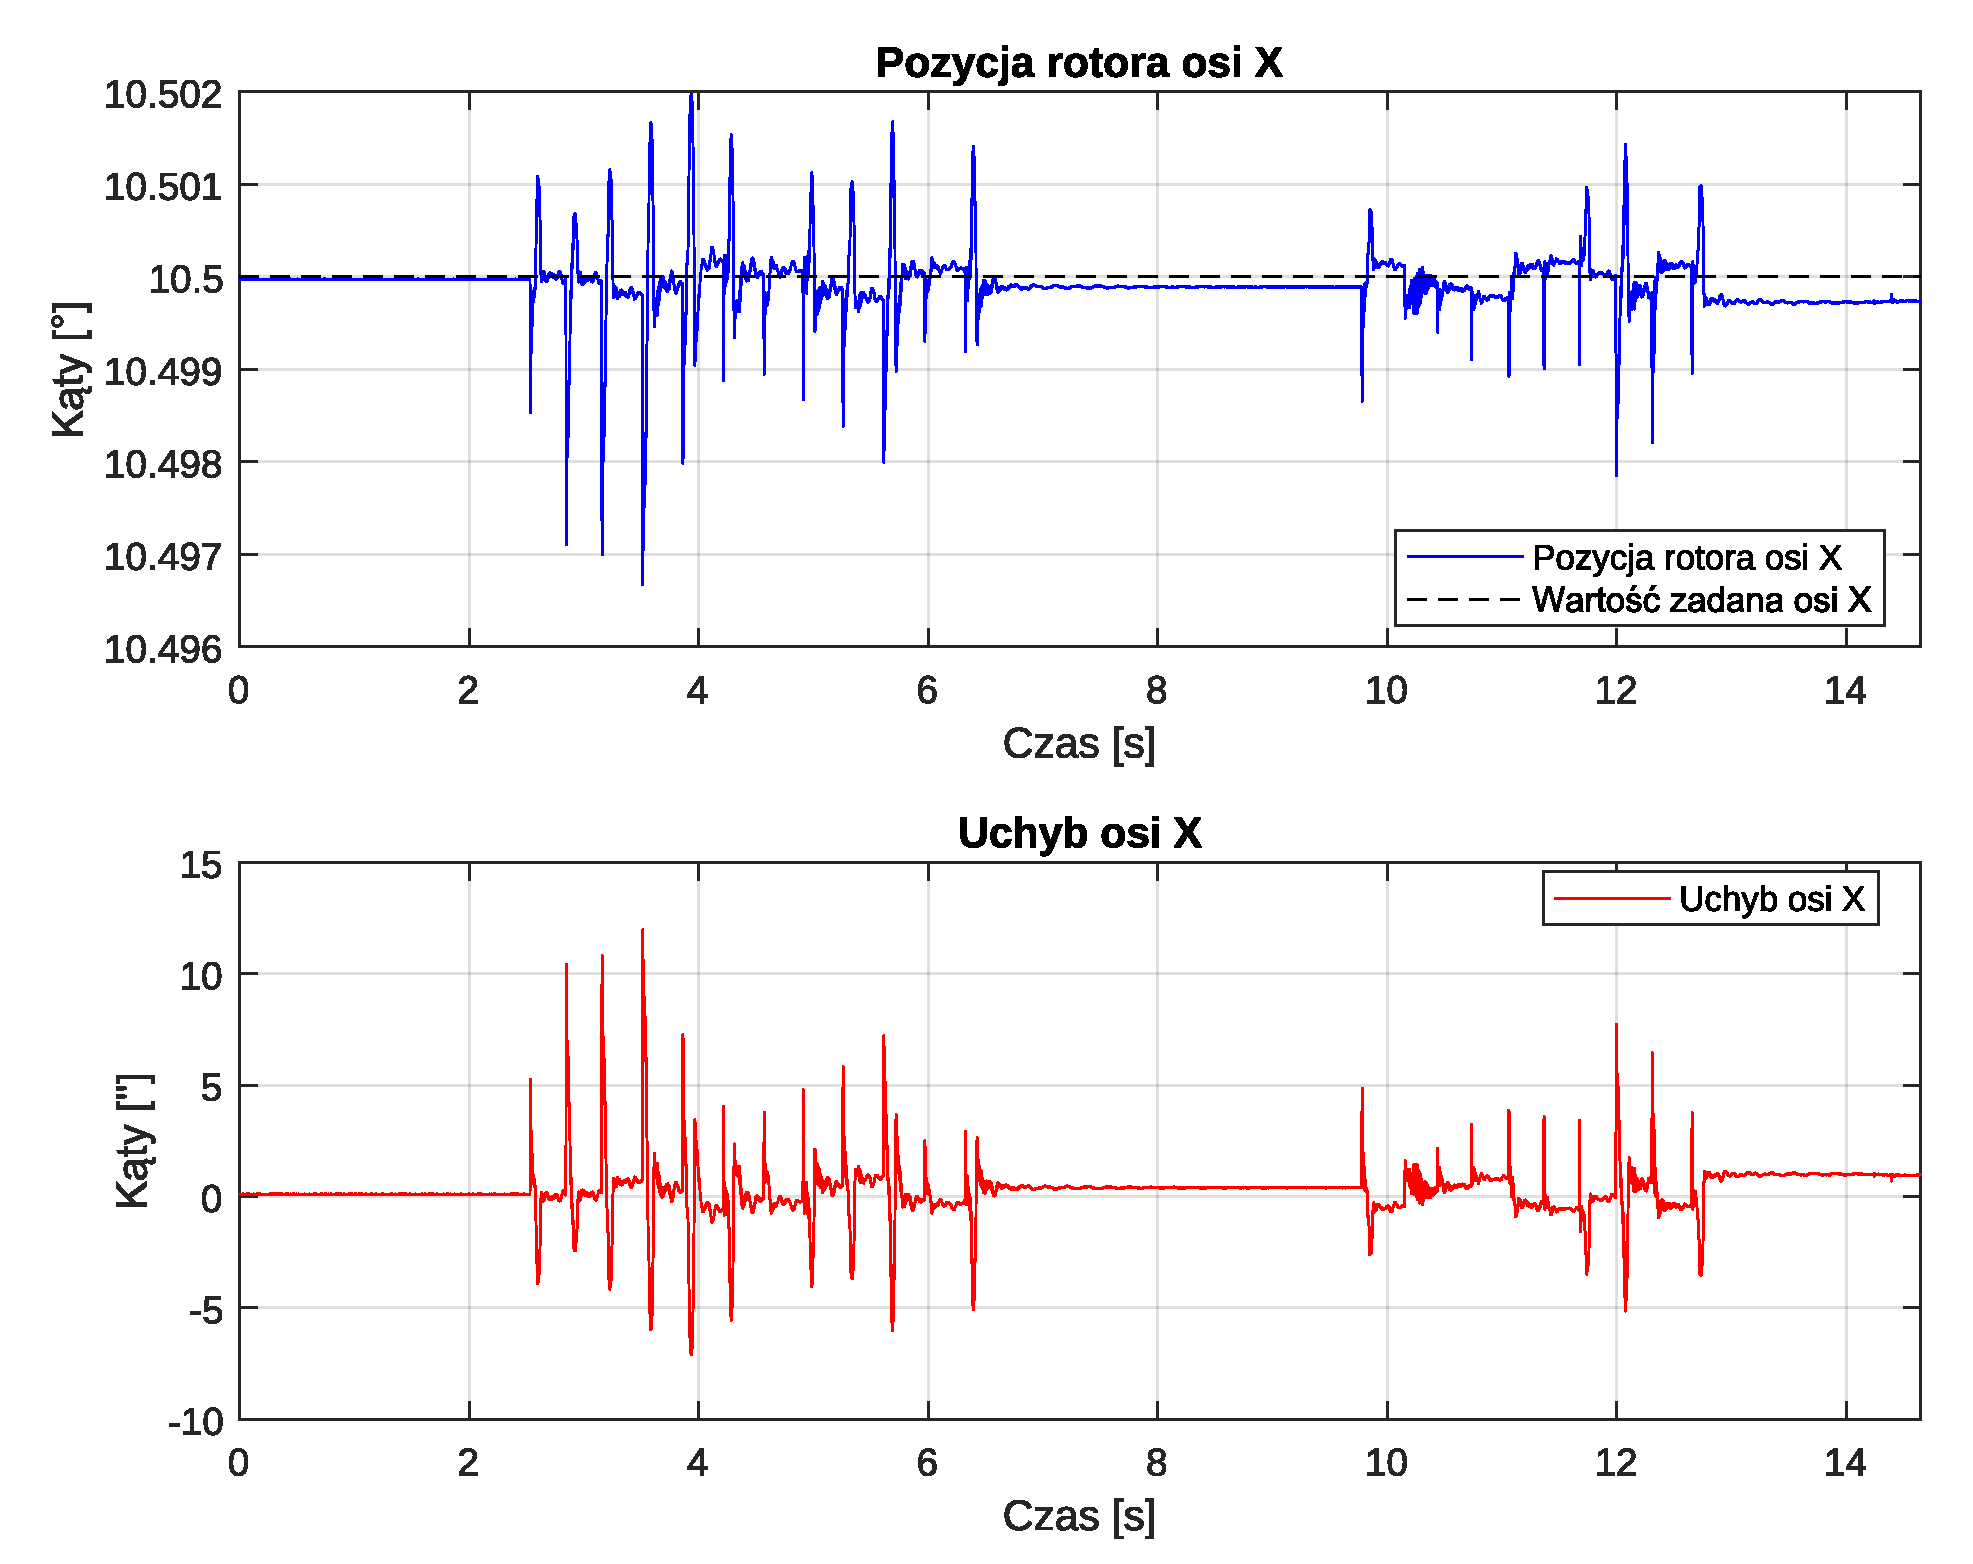
\includegraphics{testy/wykresy_inżynierka/pukanieX.pdf}}
    \caption{Przebiegi na osi X podczas zakłóceń mechanicznych.}
    \label{fig:schemat blokowy pobierania danych2}
\end{figure}

\begin{figure}[H]
    \centering
    \resizebox{12cm}{!}{
    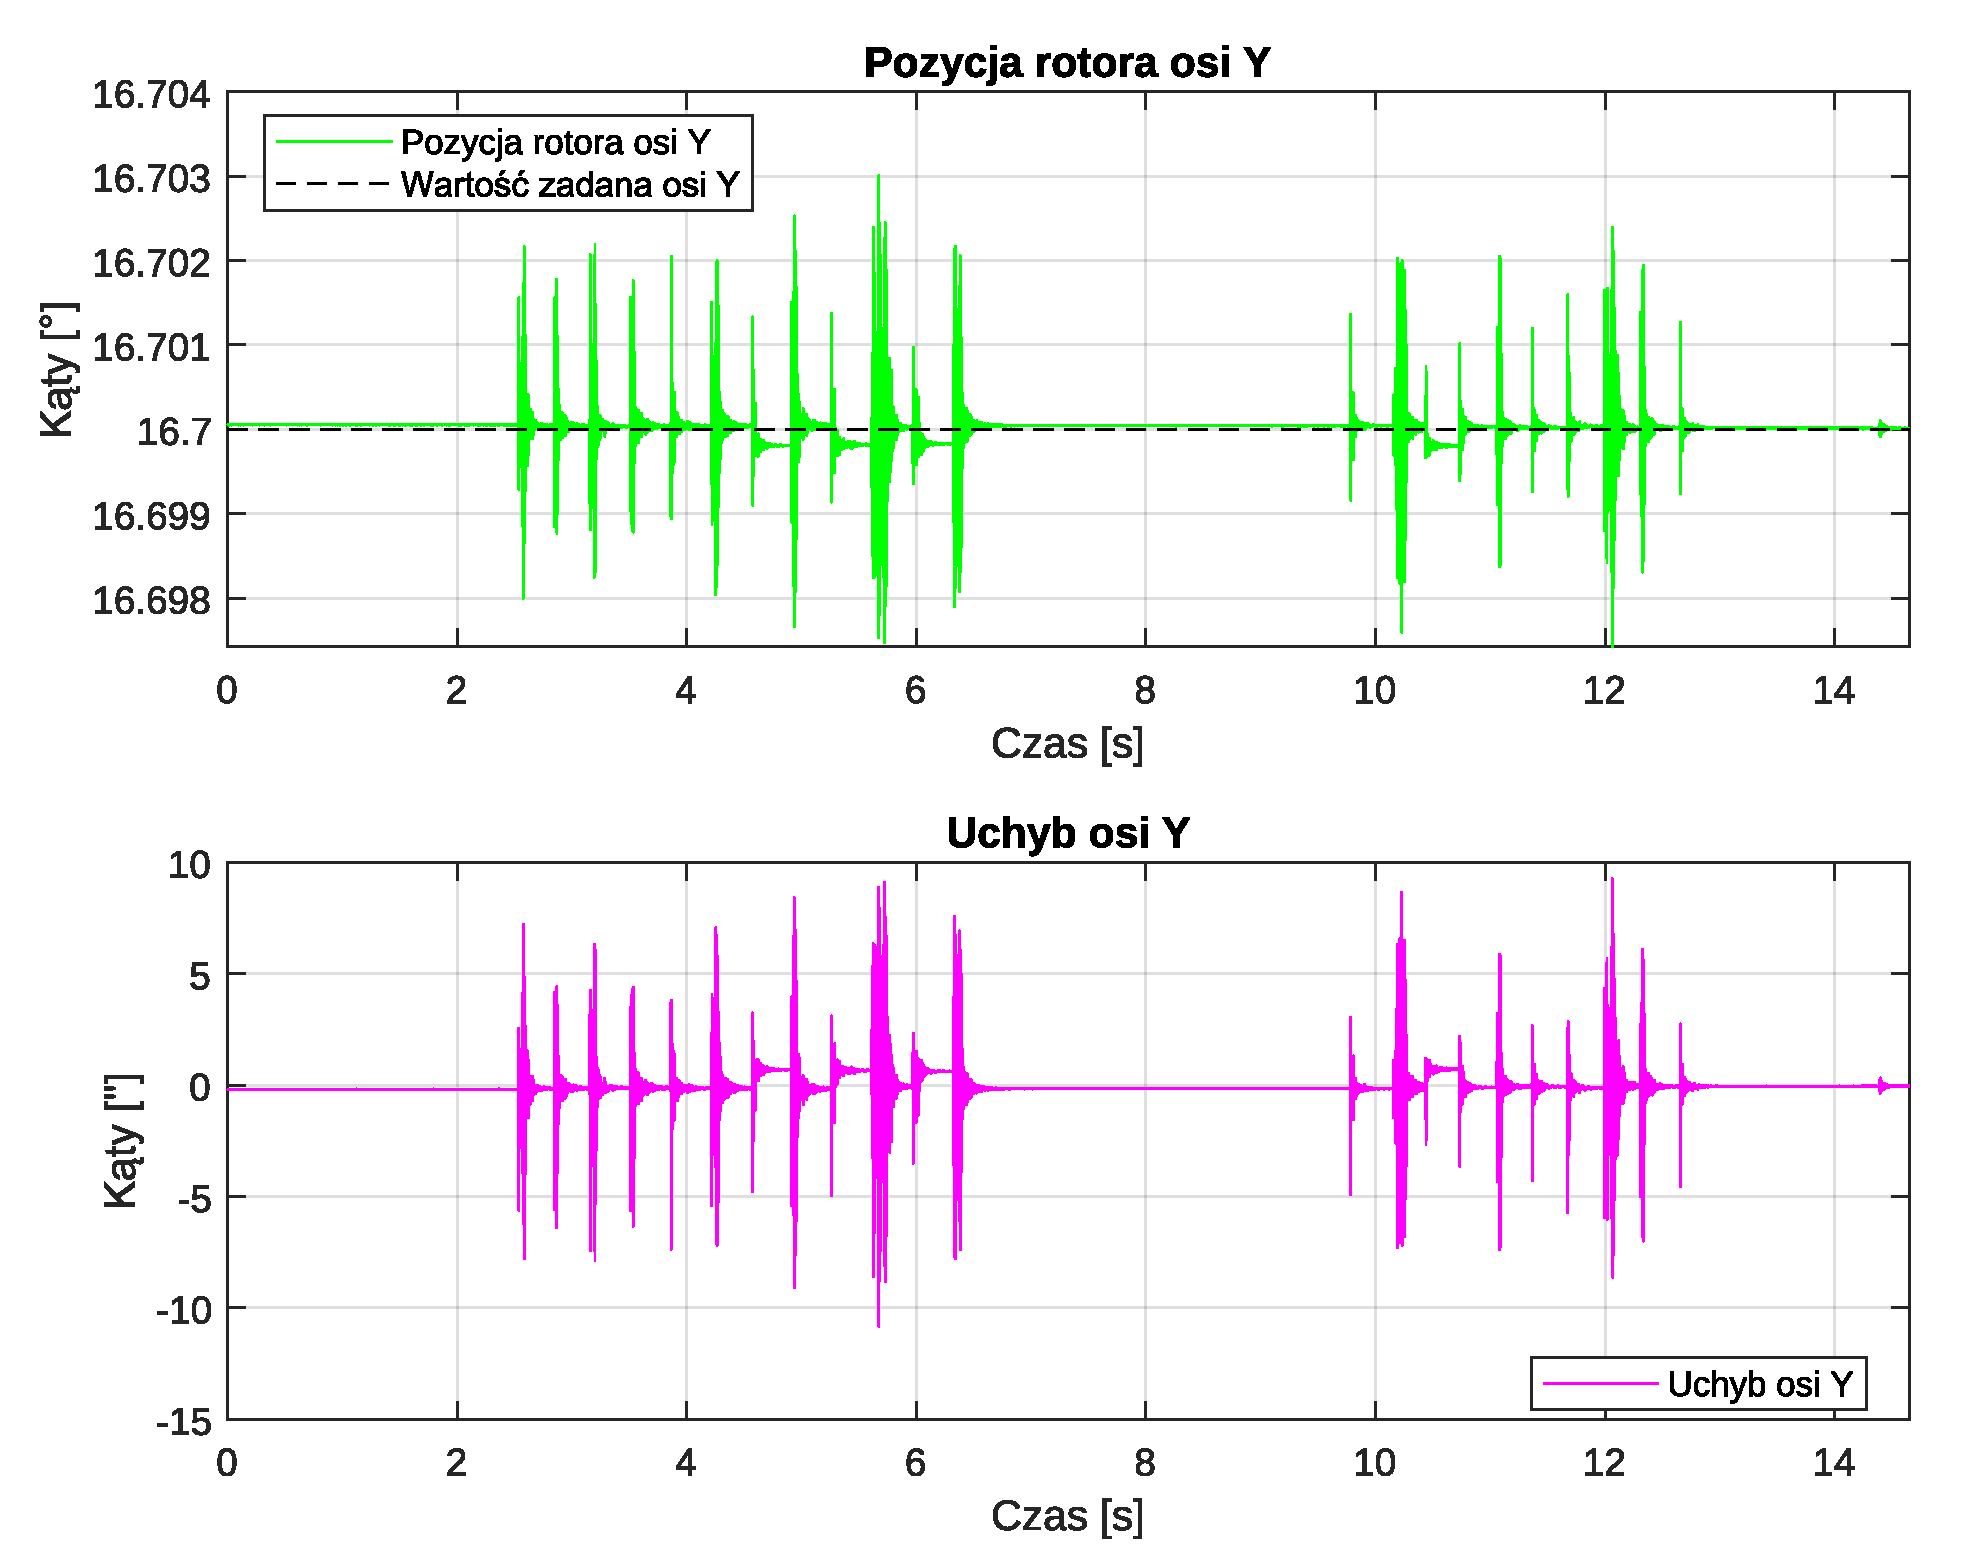
\includegraphics{testy/wykresy_inżynierka/pukanieY.pdf}}
    \caption{Przebiegi na osi Y podczas zakłóceń mechanicznych.}
    \label{fig:schemat blokowy pobierania danych2}
\end{figure}

\noindent Badano wpływ zakłócenia na jakość utrzymywania pozycji zadanej. Zakłócenia zostały wygenerowane przez delikatne uderzenia w konstrukcję w okolicach osi X. Wyniki pokazują występowanie drgań mechanicznych przenoszonych na całą konstrukcję. \newline
\noindent Po ustaniu tych drgań pozycja w obu osiach uległa niewielkiemu przesunięciu. Regulator nie przywraca pozycji zadanej, ponieważ wartość zarejestrowanego błędu położenia nie wykracza poza strefę nieczułości. Wprowadzenie tej strefy nieczułości było wymagane z uwagi na dyskretny charakter ruchu silnika krokowego oraz szumu pomiarowego pozycji.

\section{Trajektoria sinusoidalna}
W eksperymencie wykorzystano trajektorie sinusoidalne o różnych okresach takich jak: 1 s, 2 s, 5 s, 10 s i 200 s.

\begin{figure}[H]
    \centering
    \resizebox{12cm}{!}{
    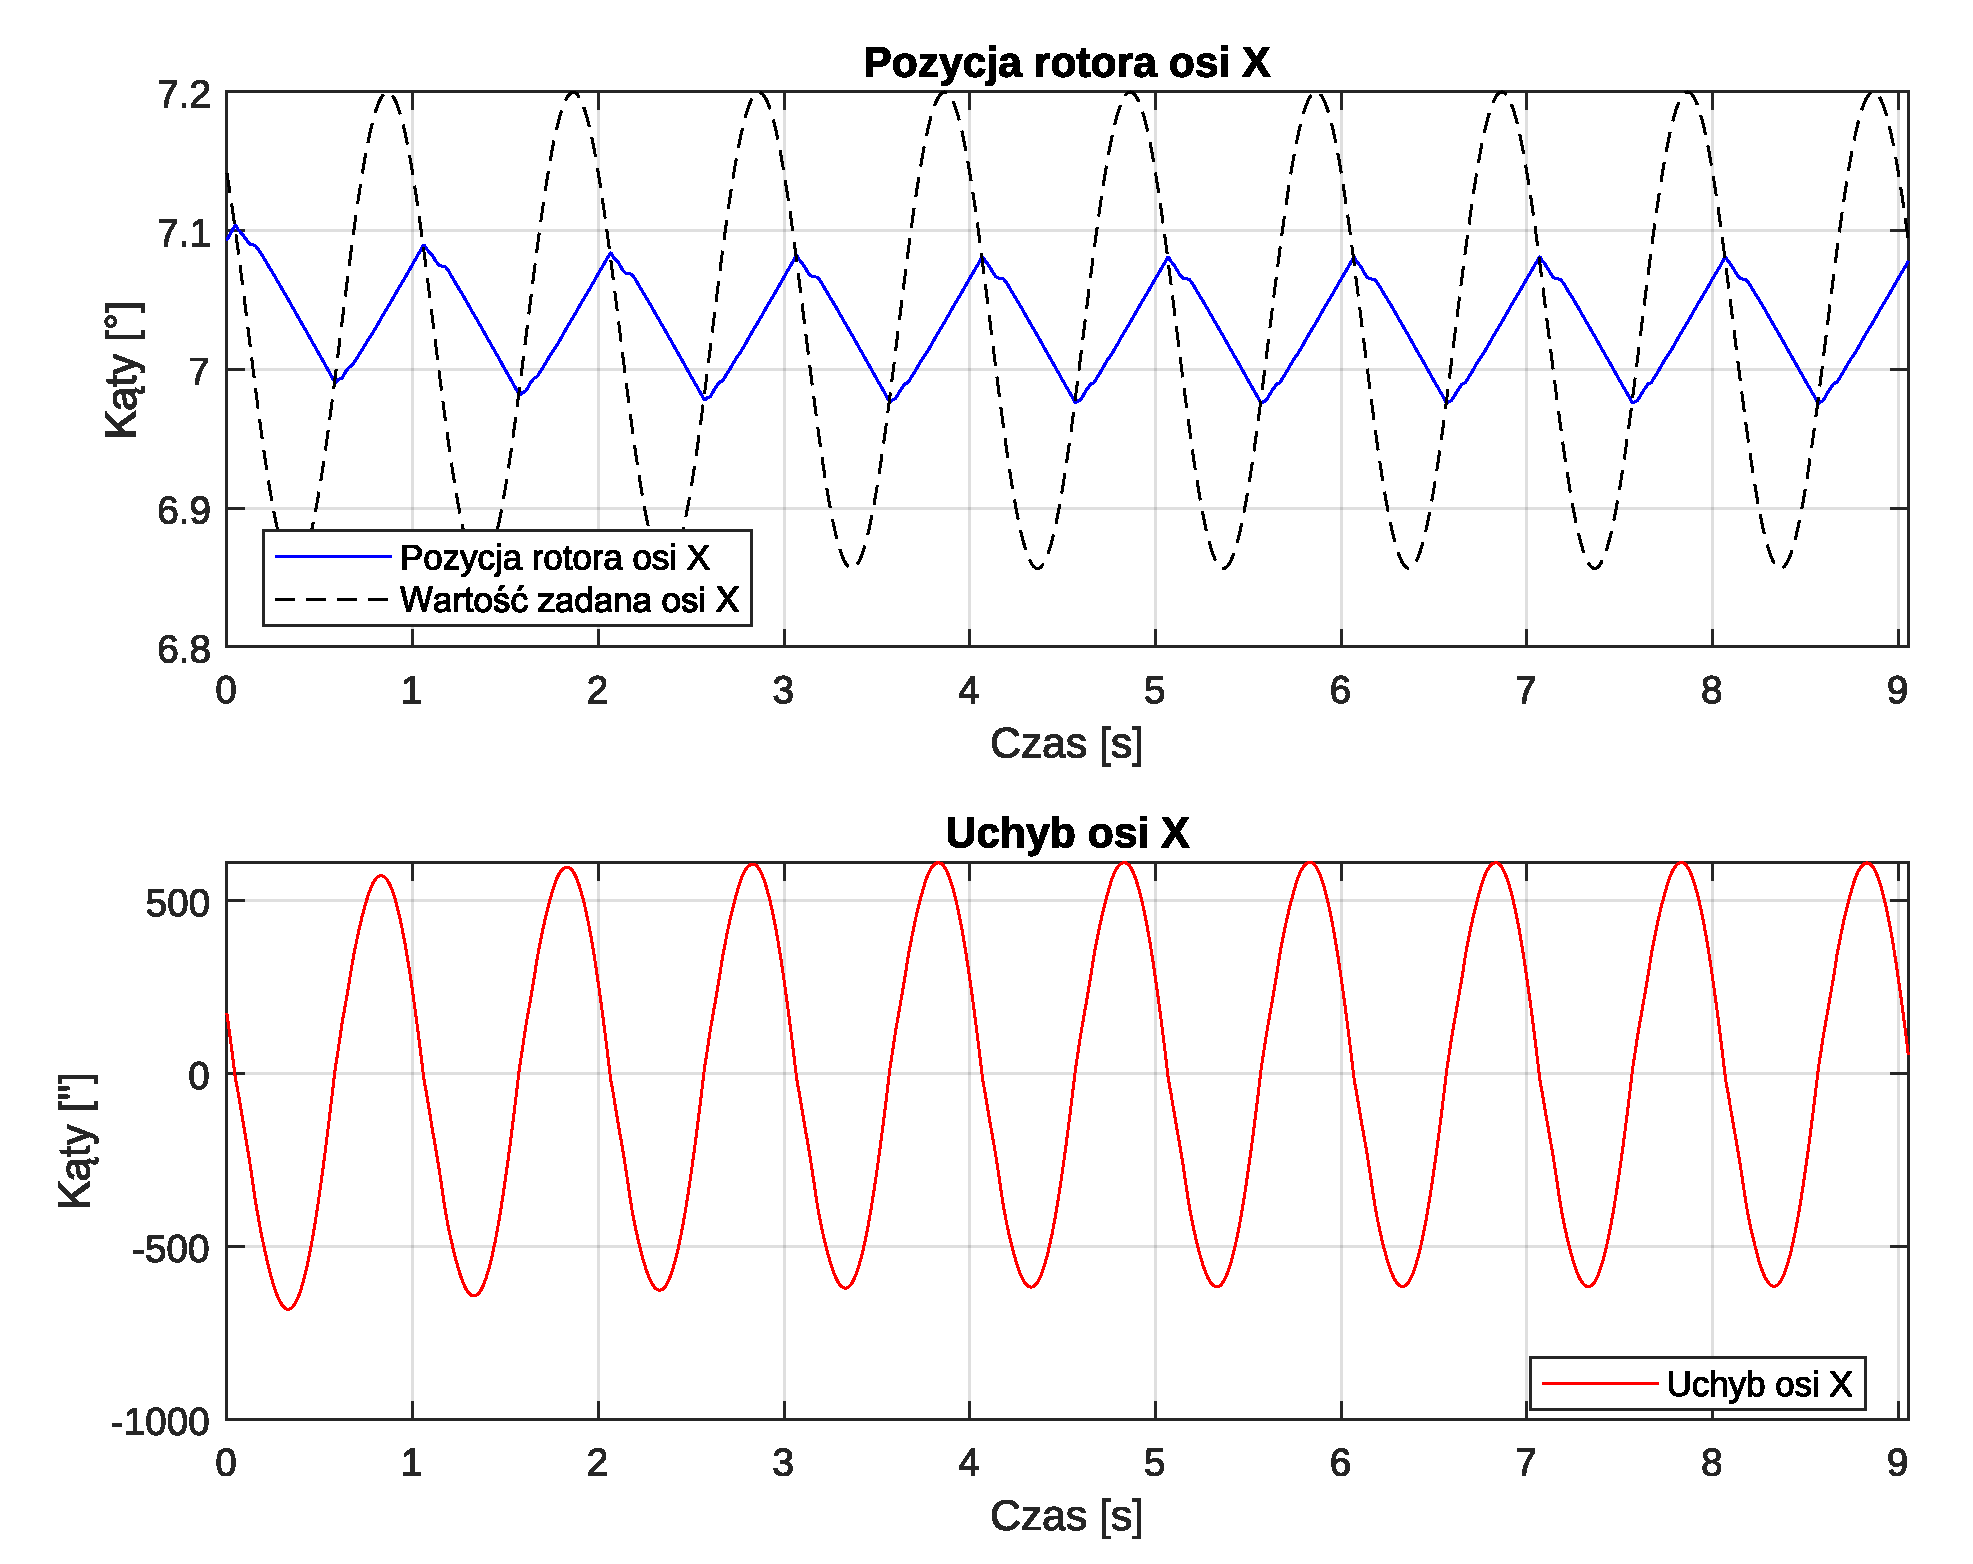
\includegraphics{testy/wykresy_inżynierka/sinus1sX.pdf}}
    \caption{Przebiegi dla trajektorii sinusoidalnej o okresie 1 sekund na osi X.}
    \label{fig:Przebiegi dla trajektorii sinusoidalnej o okresie 1 sekund na osi X.}
\end{figure}

\begin{figure}[H]
    \centering
    \resizebox{12cm}{!}{
    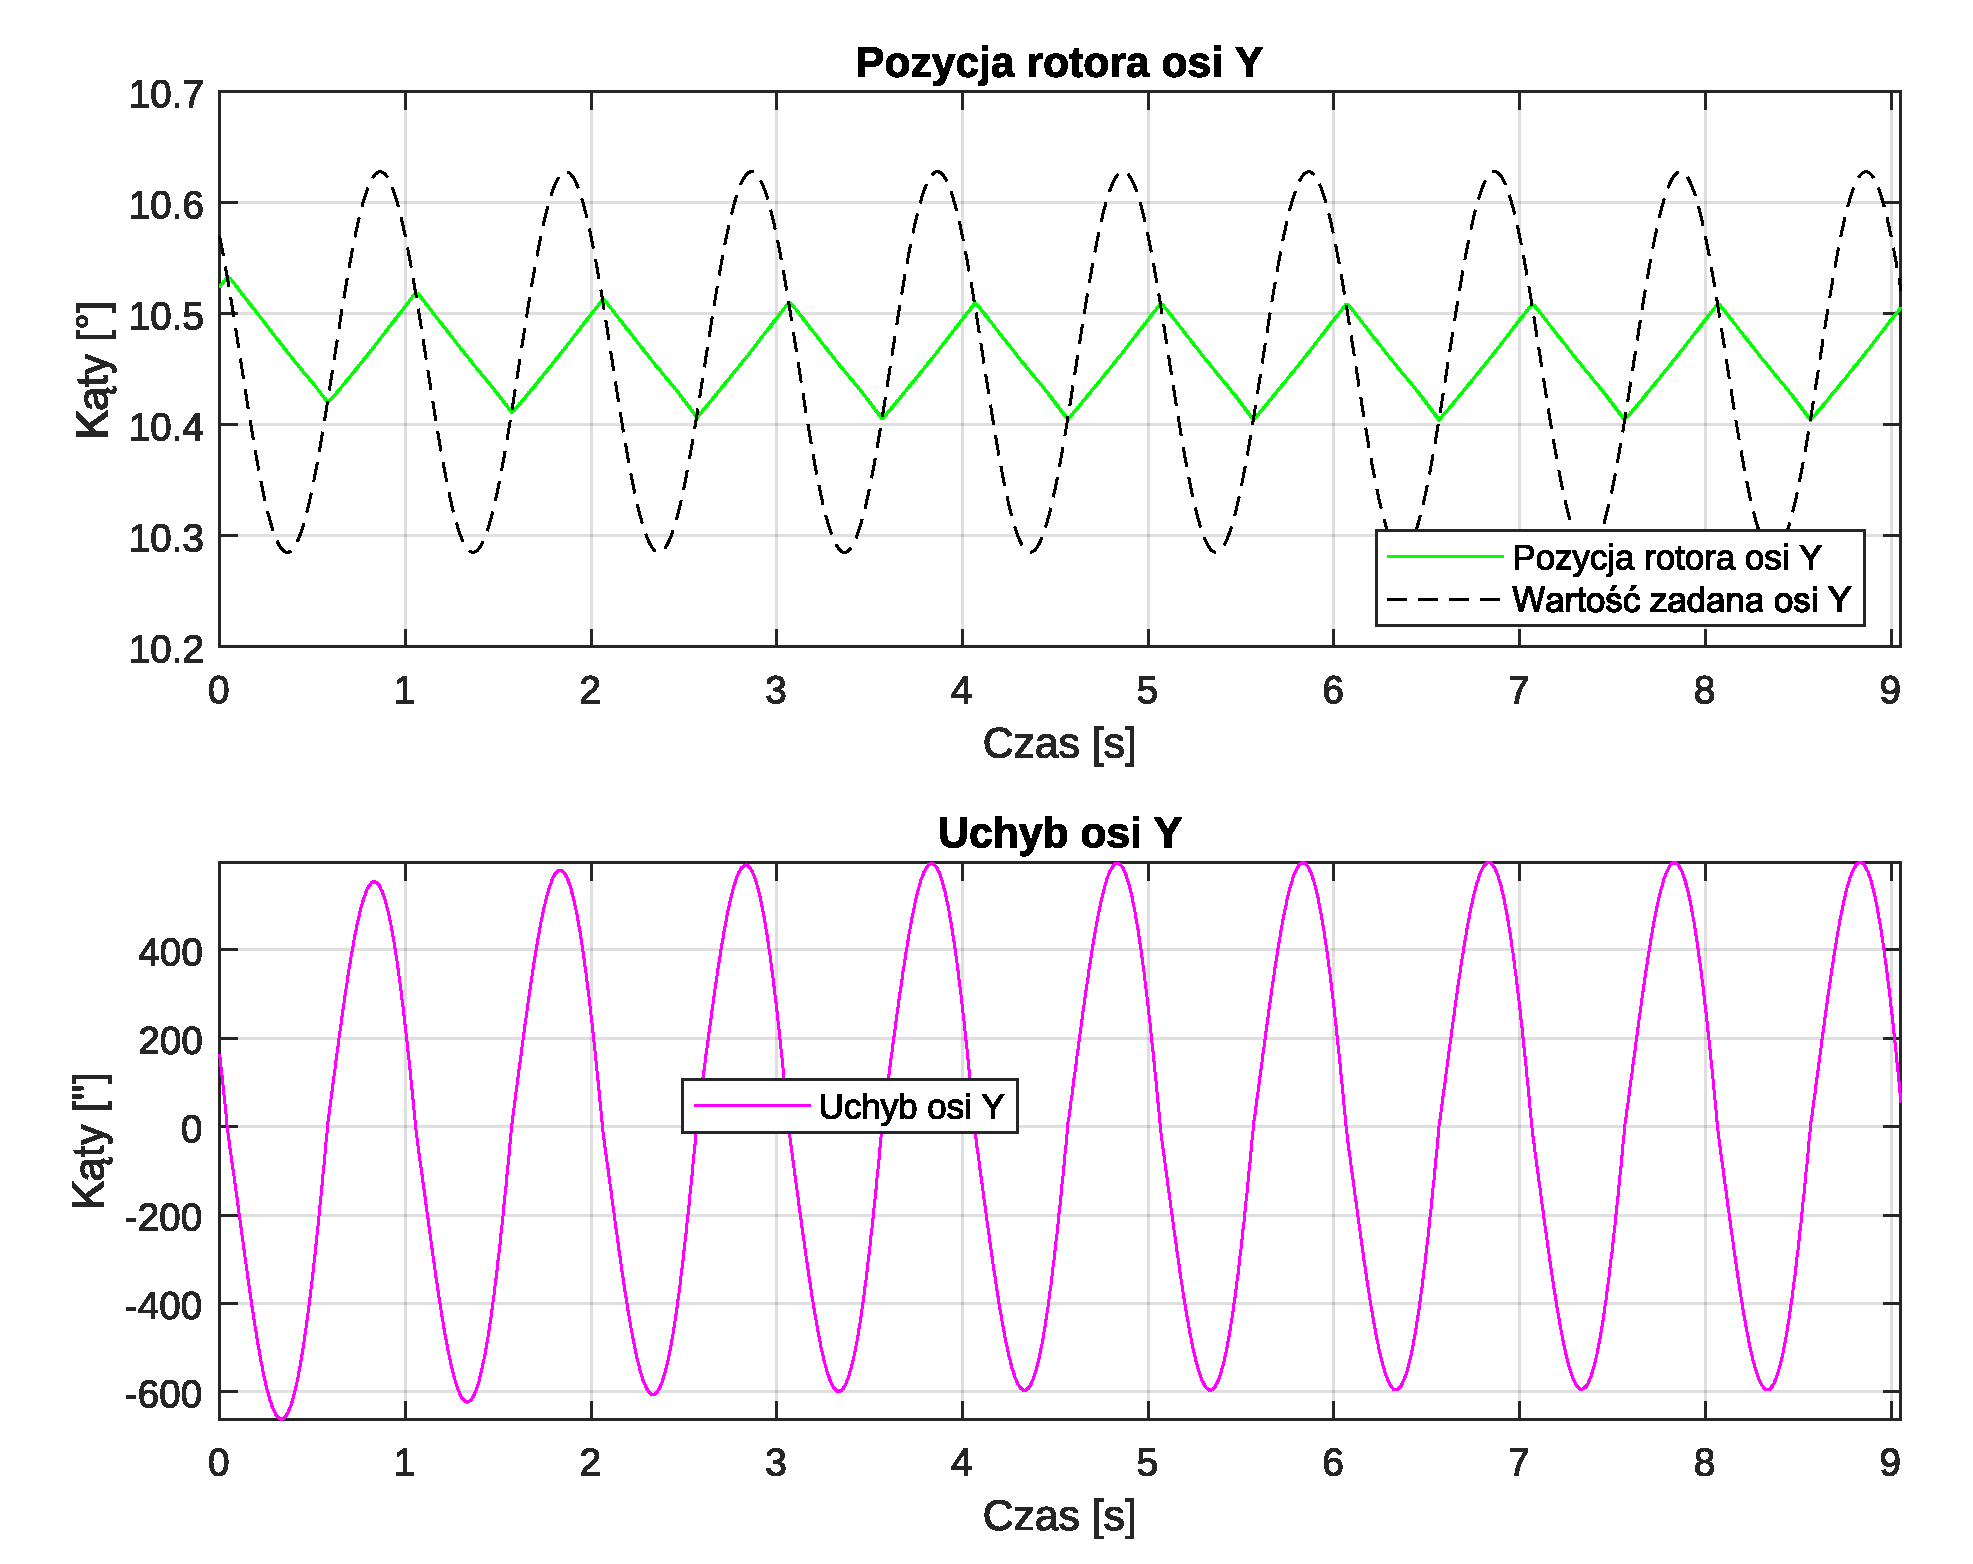
\includegraphics{testy/wykresy_inżynierka/sinus1sY.pdf}}
    \caption{Przebiegi dla trajektorii sinusoidalnej o okresie 1 sekund na osi Y.}
    \label{fig:Przebiegi dla trajektorii sinusoidalnej o okresie 1 sekund na osi Y.}
\end{figure}

\begin{figure}[H]
    \centering
    \resizebox{12cm}{!}{
    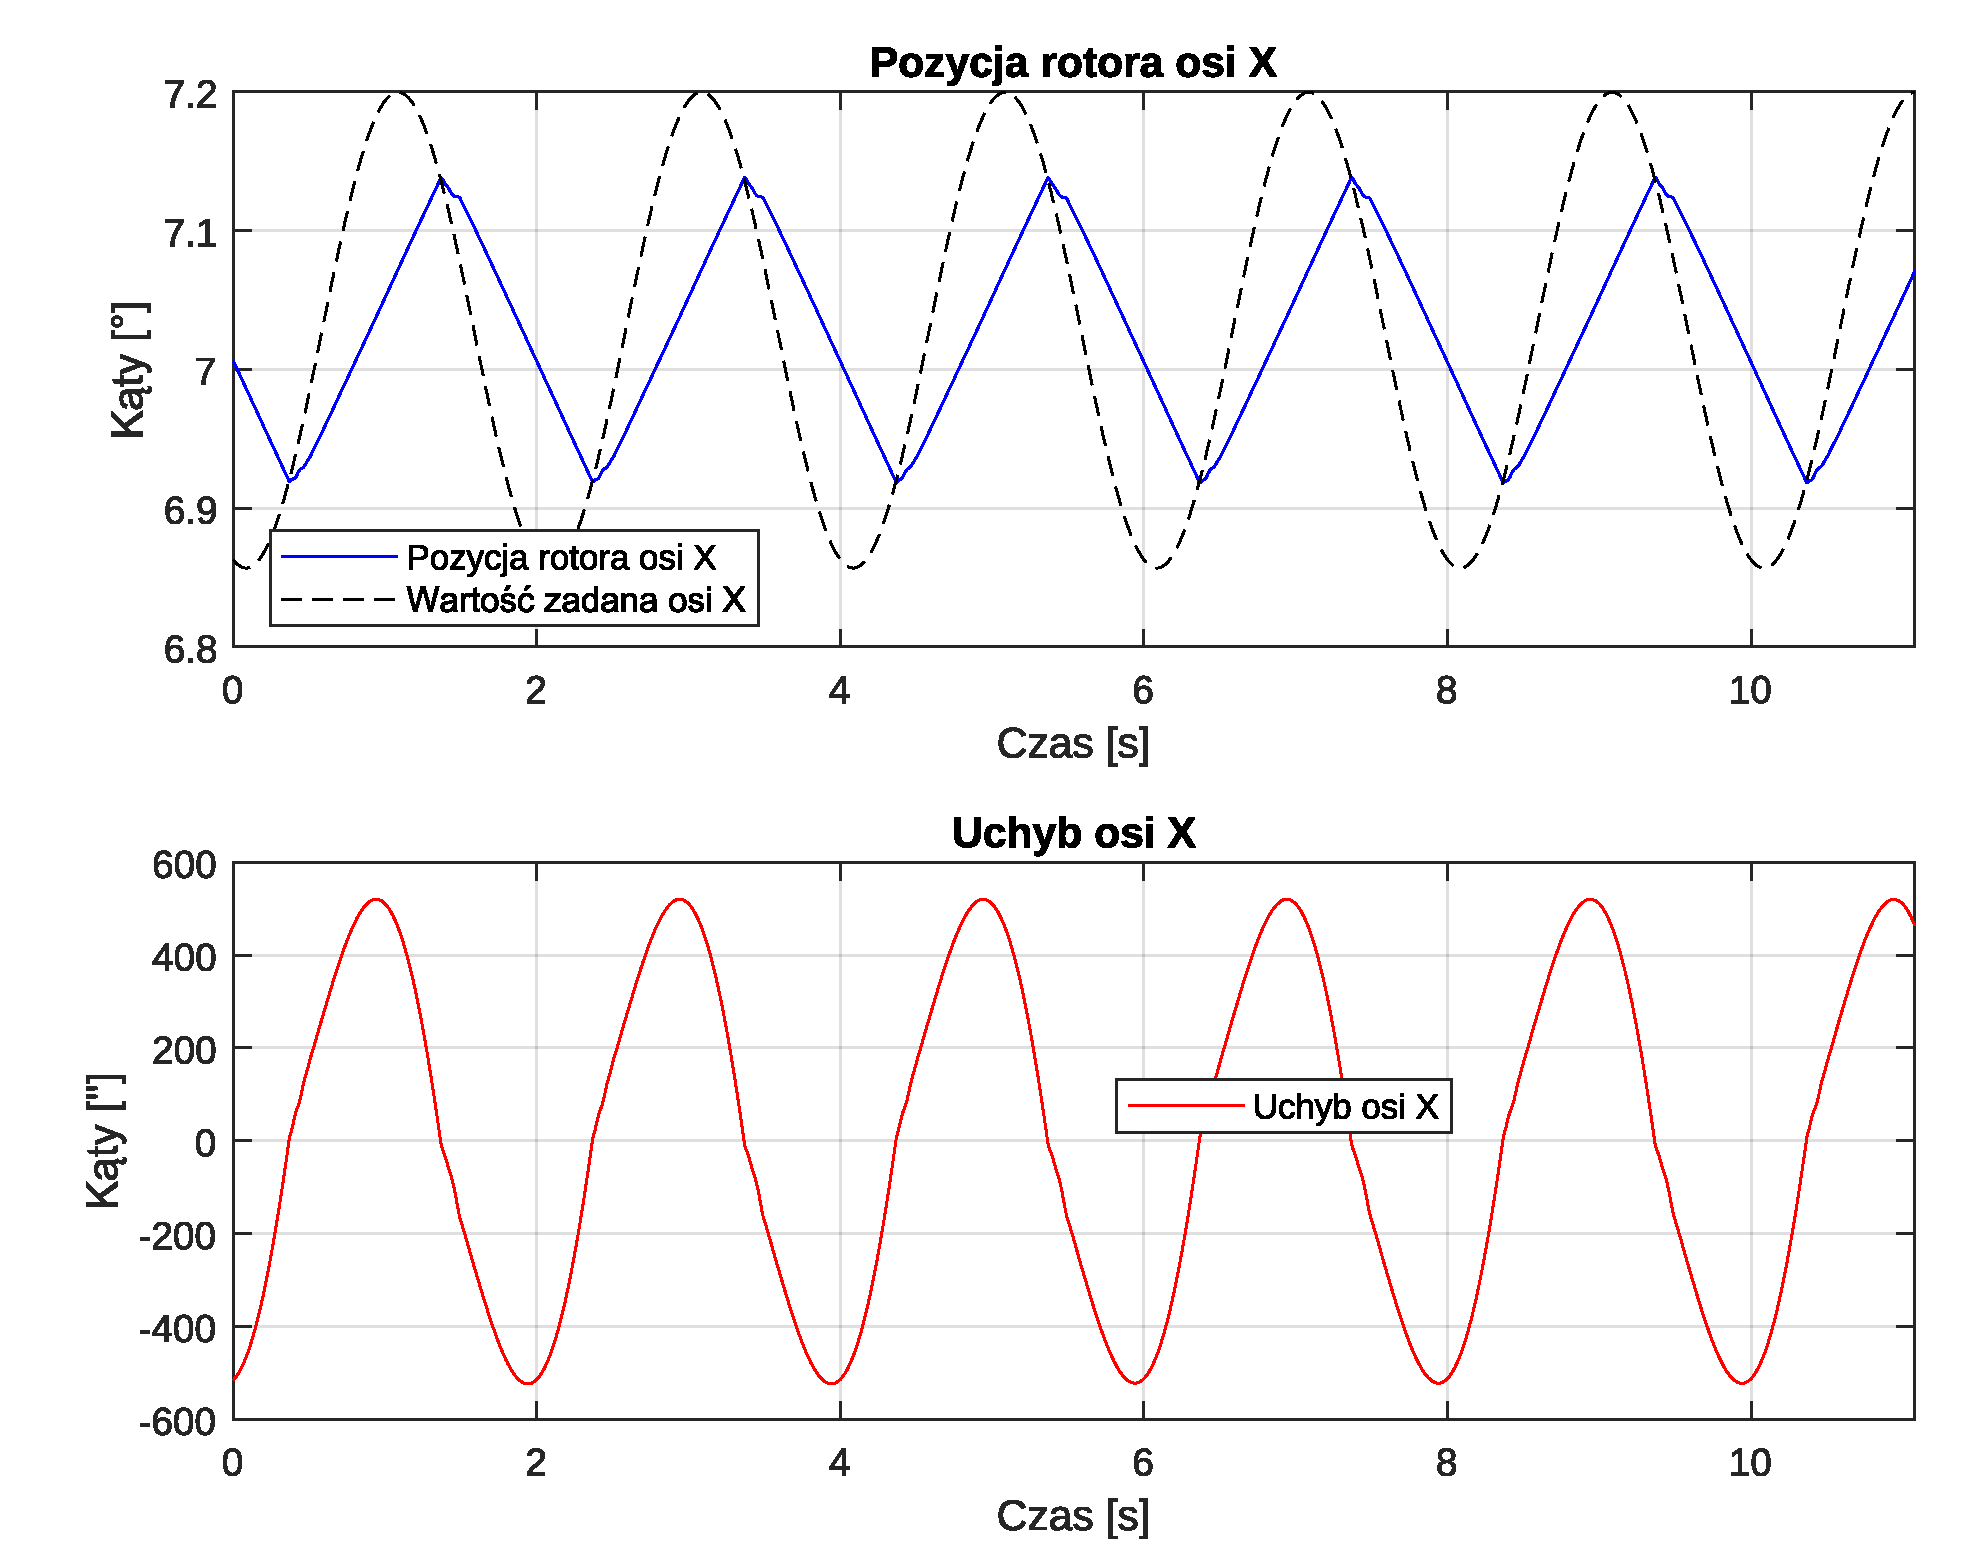
\includegraphics{testy/wykresy_inżynierka/sinus2sX.pdf}}
    \label{fig:schemat blokowy pobierania danych2}
    \caption{Przebiegi dla trajektorii sinusoidalnej o okresie 2 sekund na osi X.}
\end{figure}

\begin{figure}[H]
    \centering
    \resizebox{12cm}{!}{
    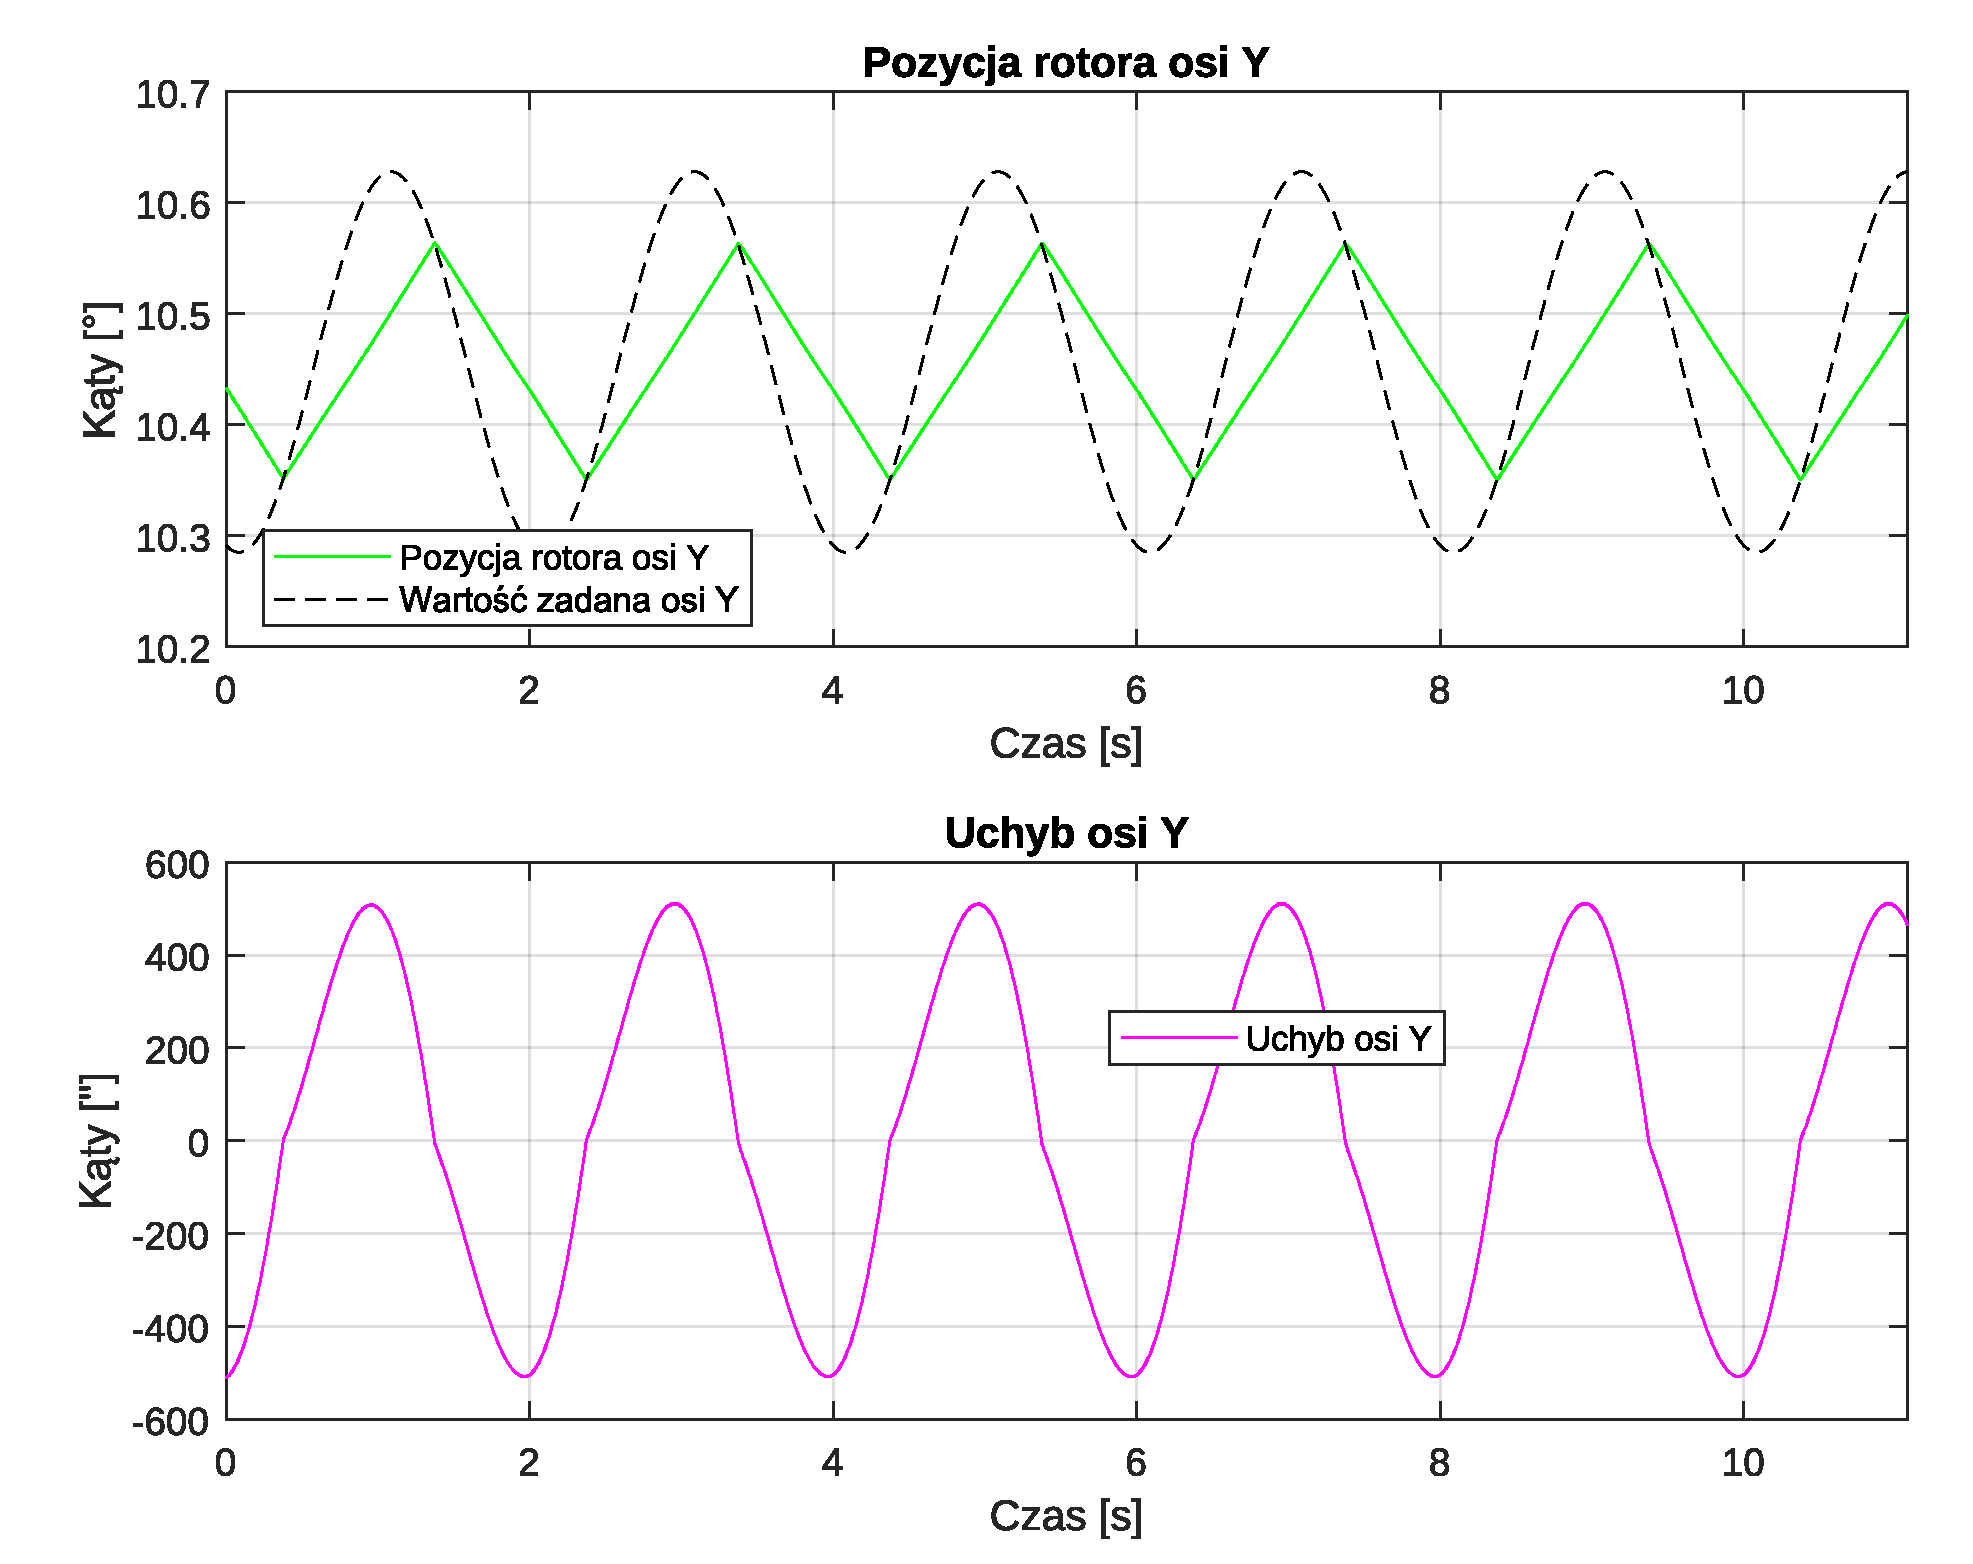
\includegraphics{testy/wykresy_inżynierka/sinus2sY.pdf}}
    \label{fig:schemat blokowy pobierania danych2}
    \caption{Przebiegi dla trajektorii sinusoidalnej o okresie 2 sekund na osi Y.}
\end{figure}

\begin{figure}[H]
    \centering
    \resizebox{12cm}{!}{
    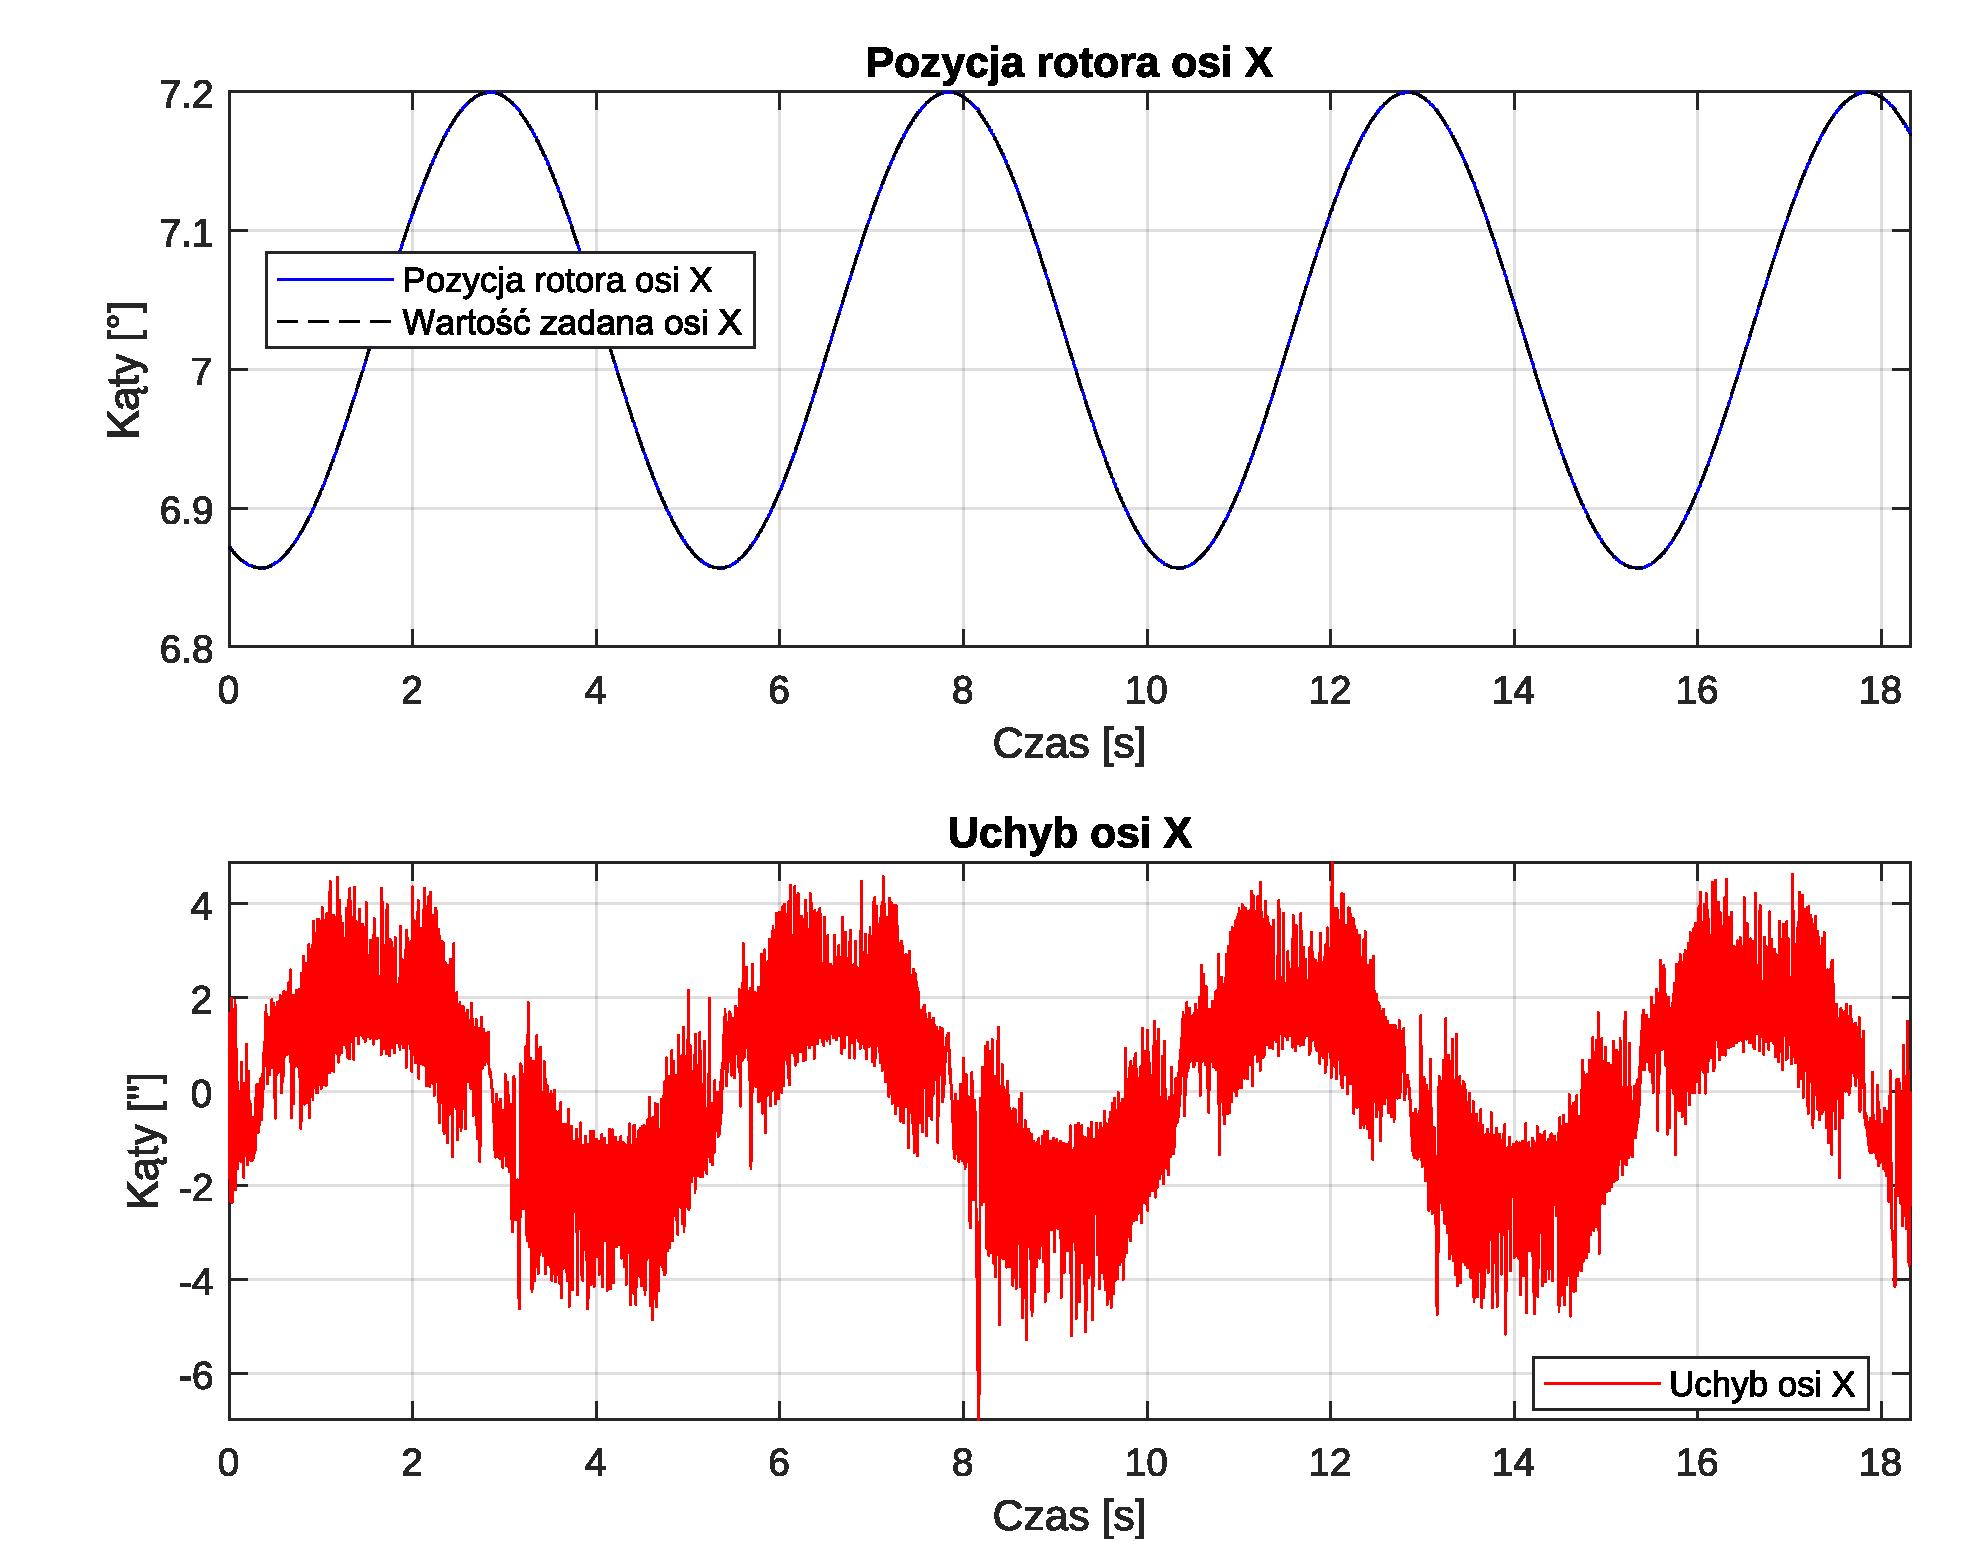
\includegraphics{testy/wykresy_inżynierka/sinus5sX.pdf}}
    \caption{Przebiegi dla trajektorii sinusoidalnej o okresie 5 sekund na osi X.}
    \label{fig:schemat blokowy pobierania danych2}
\end{figure}

\begin{figure}[H]
    \centering
    \resizebox{12cm}{!}{
    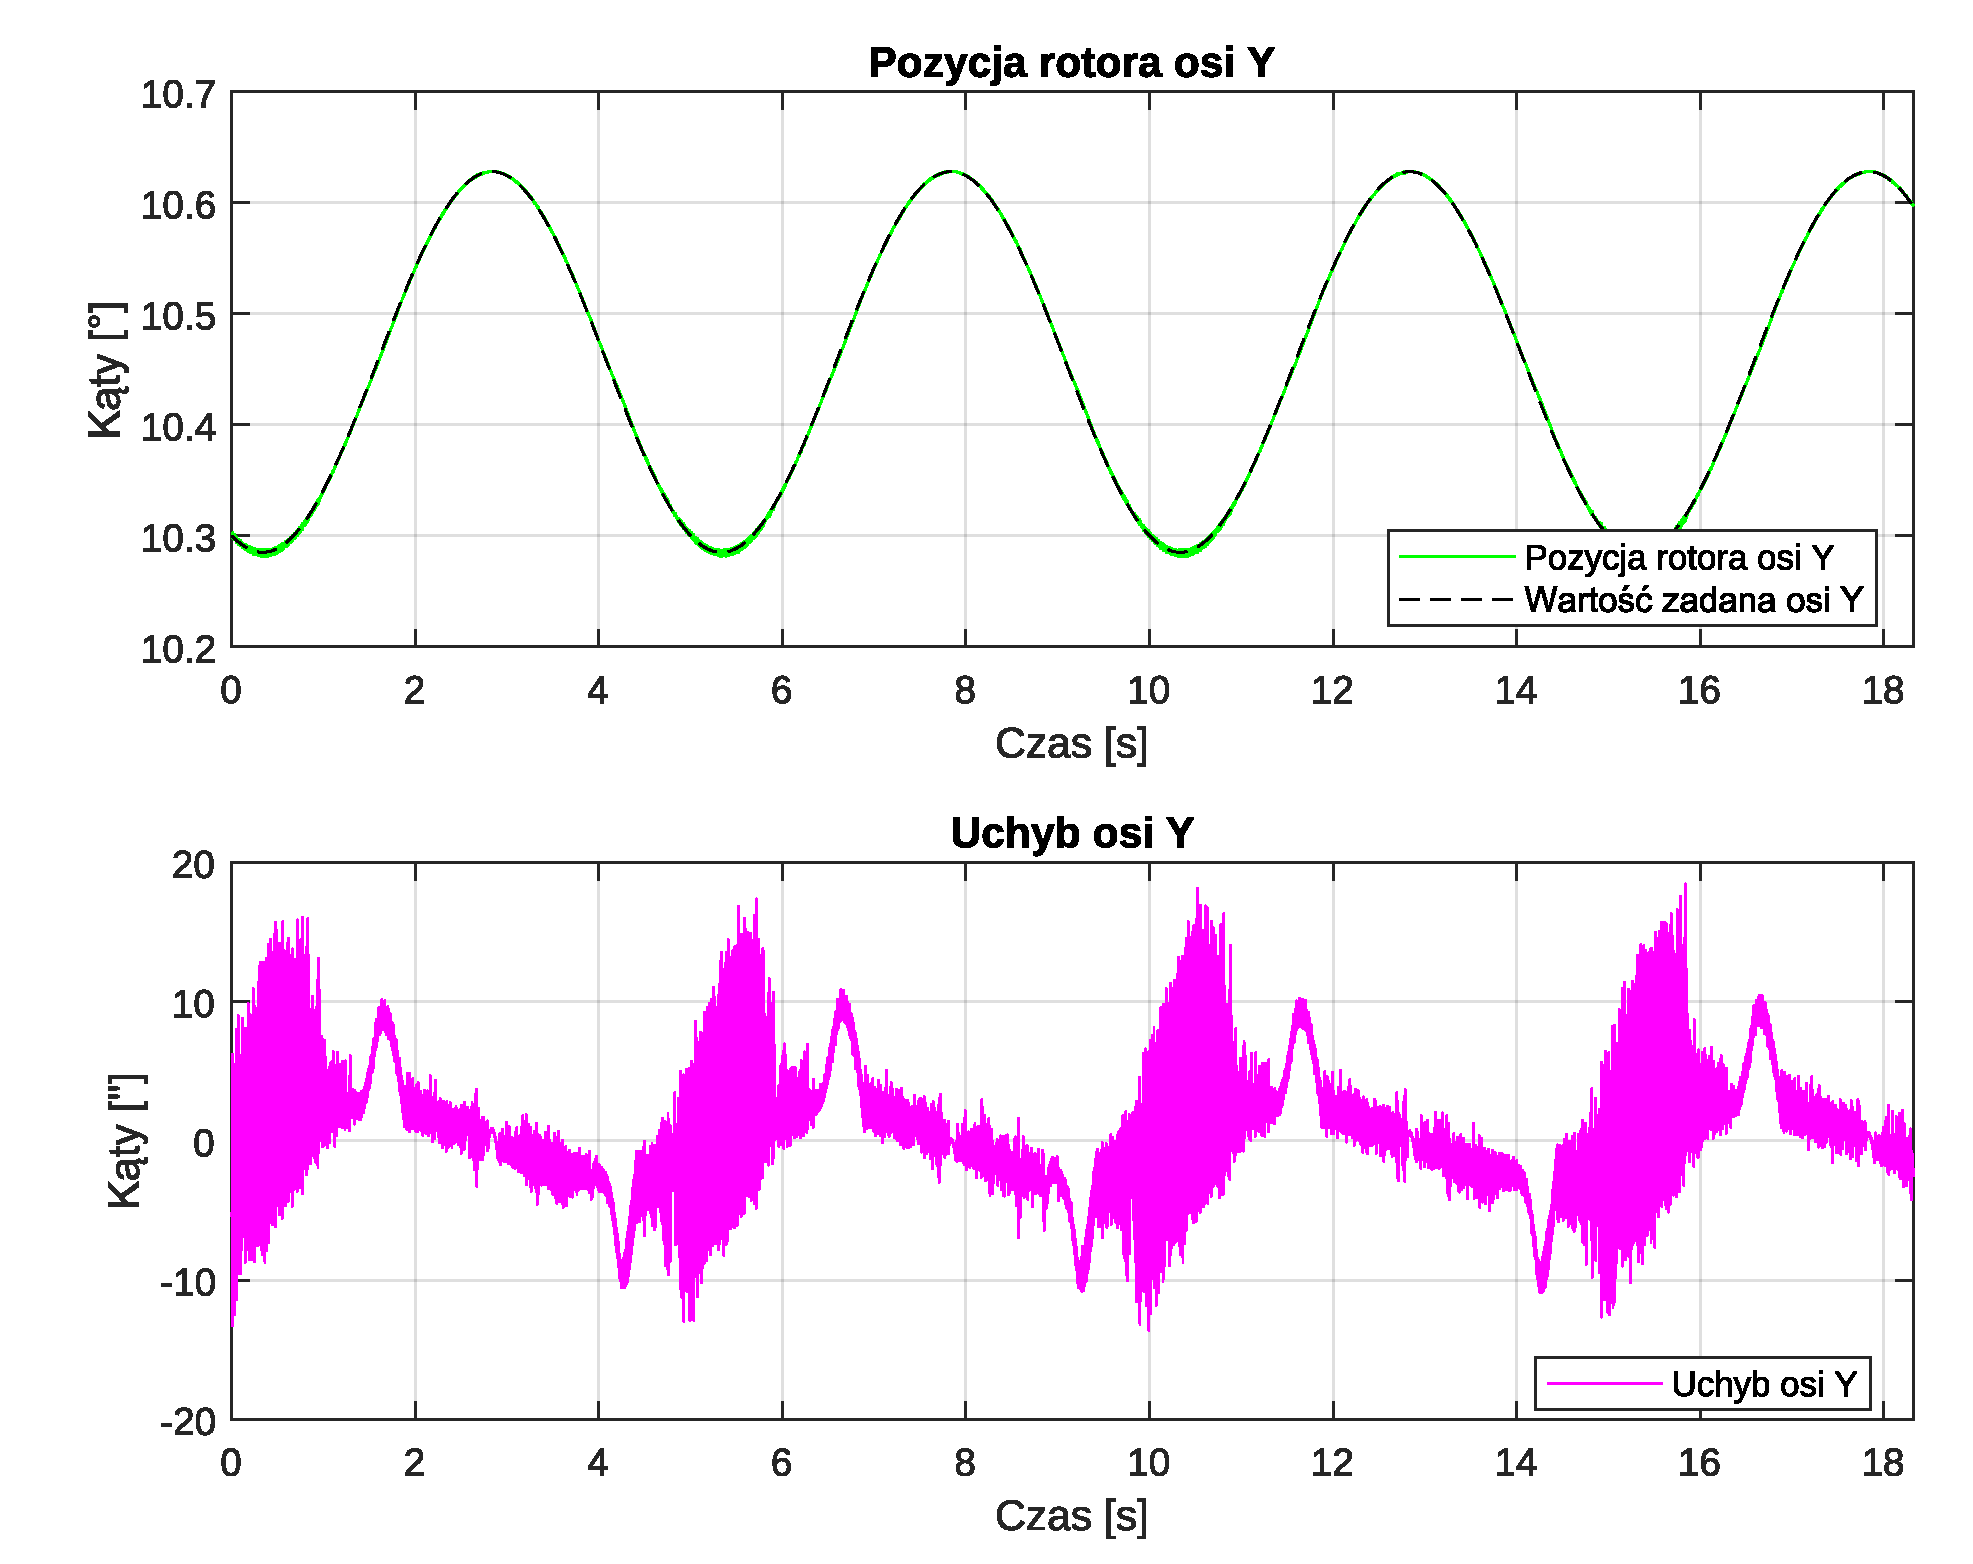
\includegraphics{testy/wykresy_inżynierka/sinus5sY.pdf}}
    \caption{Przebiegi dla trajektorii sinusoidalnej o okresie 5 sekund na osi Y.}
    \label{fig:schemat blokowy pobierania danych2}
\end{figure}

\begin{figure}[H]
    \centering
    \resizebox{12cm}{!}{
    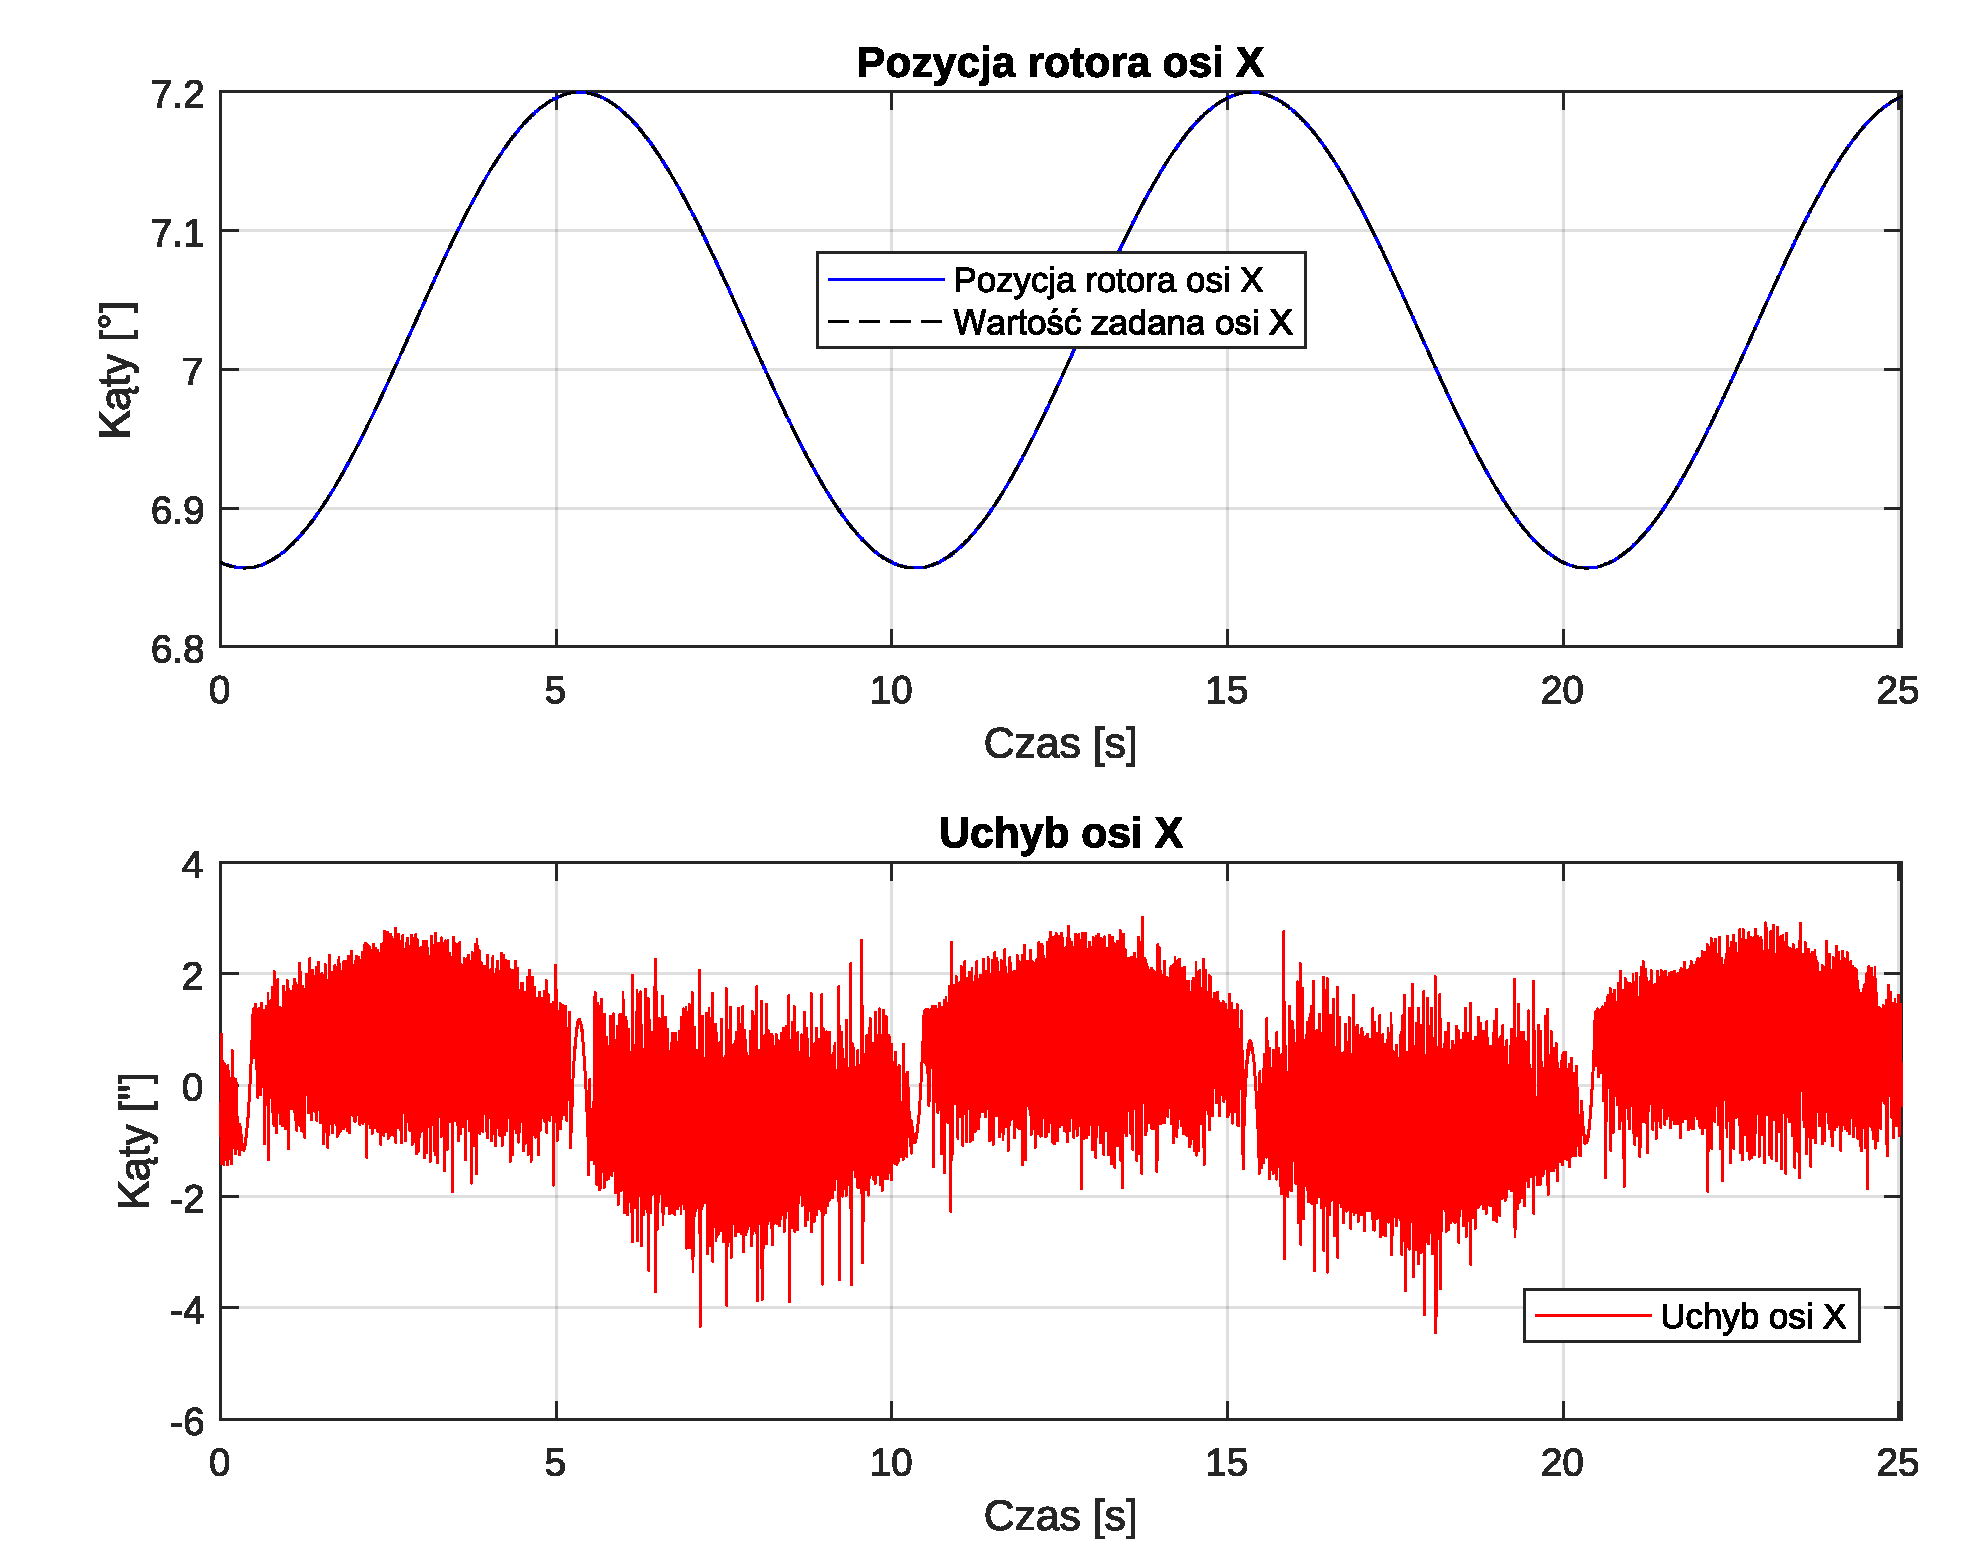
\includegraphics{testy/wykresy_inżynierka/sinus10sX.pdf}}
    \label{fig:schemat blokowy pobierania danych2}
    \caption{Przebiegi dla trajektorii sinusoidalnej o okresie 10 sekund na osi X.}
\end{figure}

\begin{figure}[H]
    \centering
    \resizebox{12cm}{!}{
    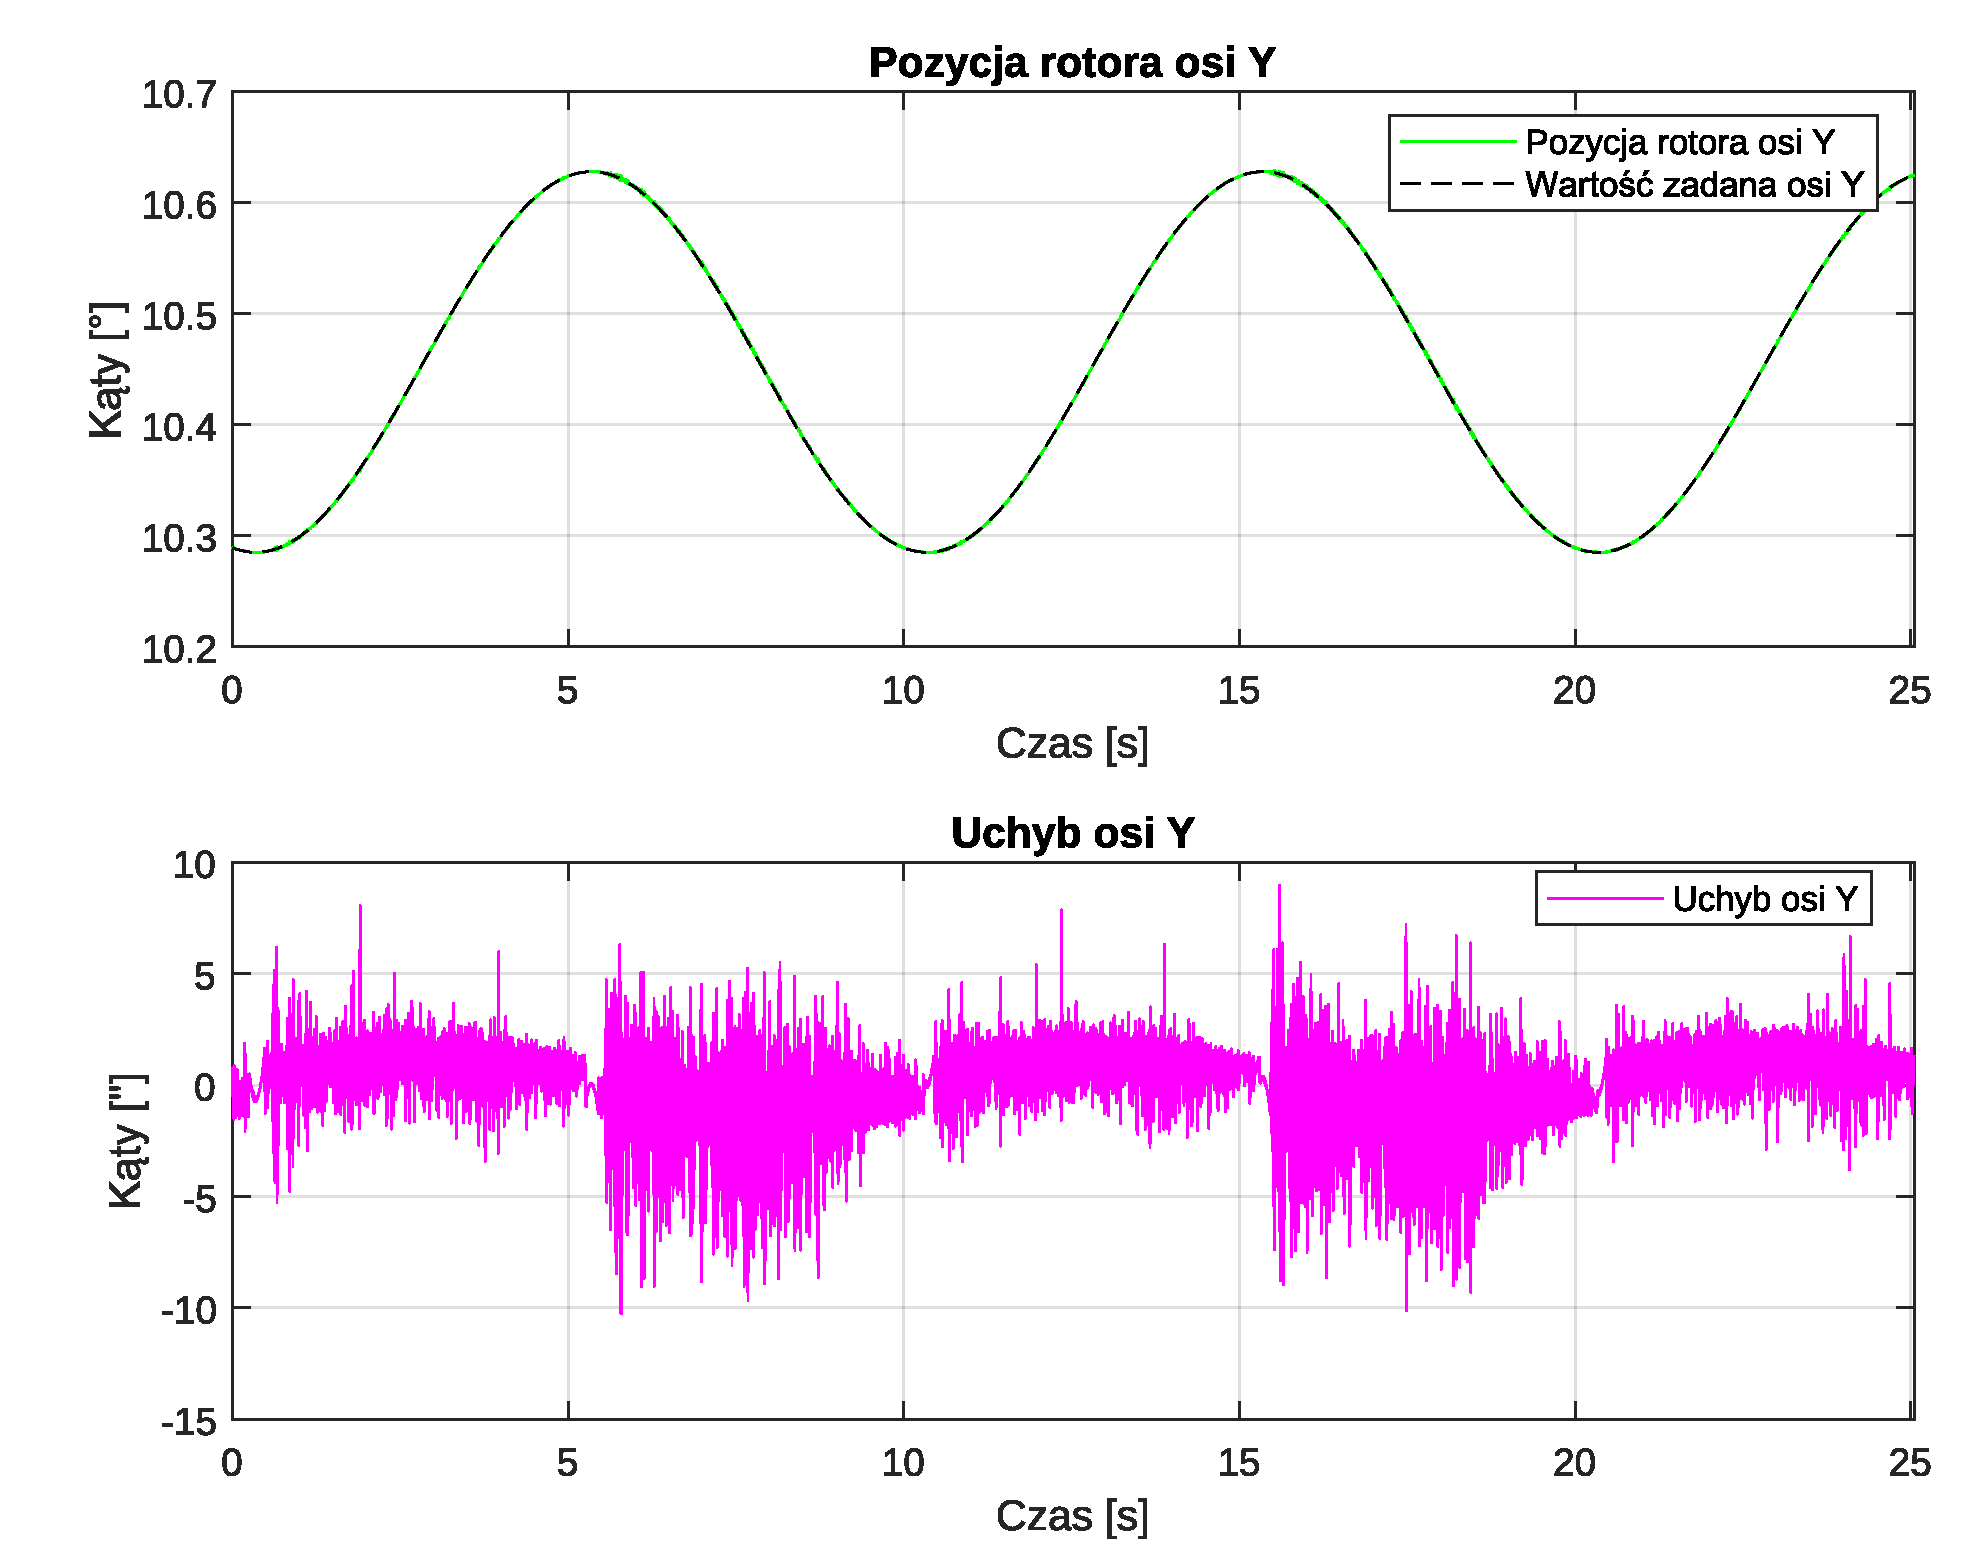
\includegraphics{testy/wykresy_inżynierka/sinus10sY.pdf}}
    \label{fig:schemat blokowy pobierania danych2}
    \caption{Przebiegi dla trajektorii sinusoidalnej o okresie 10 sekund na osi Y.}
\end{figure}

\begin{figure}[H]
    \centering
    \resizebox{12cm}{!}{
    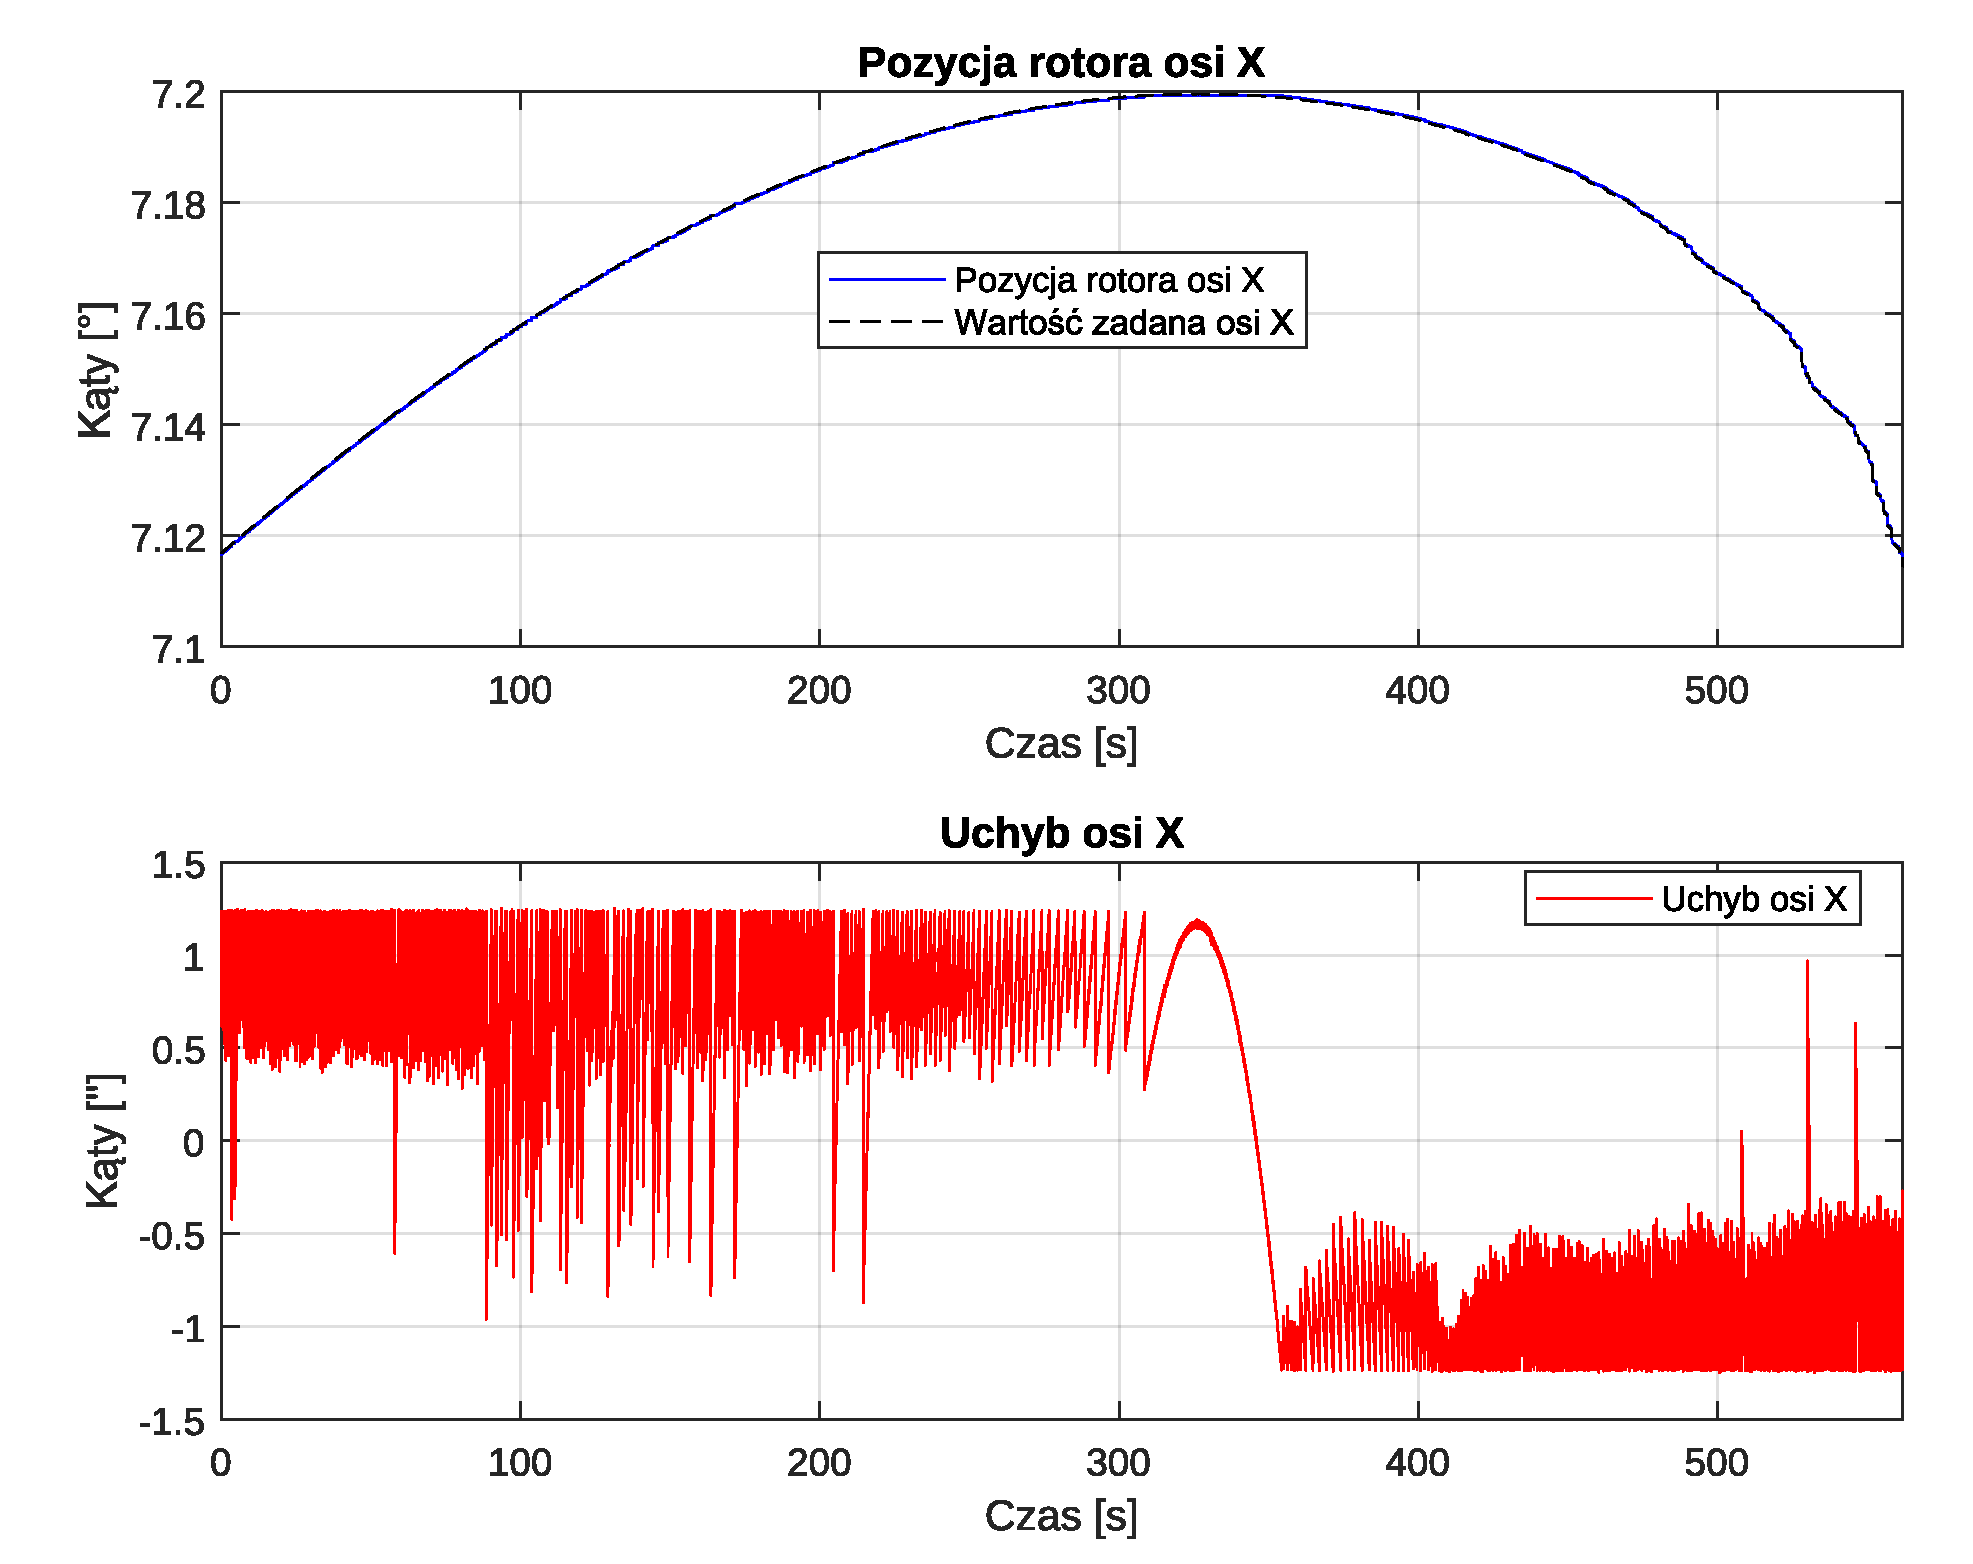
\includegraphics{testy/wykresy_inżynierka/sinus200slongX.pdf}}
    \label{fig:schemat blokowy pobierania danych2}
    \caption{Przebiegi dla trajektorii sinusoidalnej o okresie 200 sekund na osi X.}
\end{figure}

\begin{figure}[H]
    \centering
    \resizebox{12cm}{!}{
    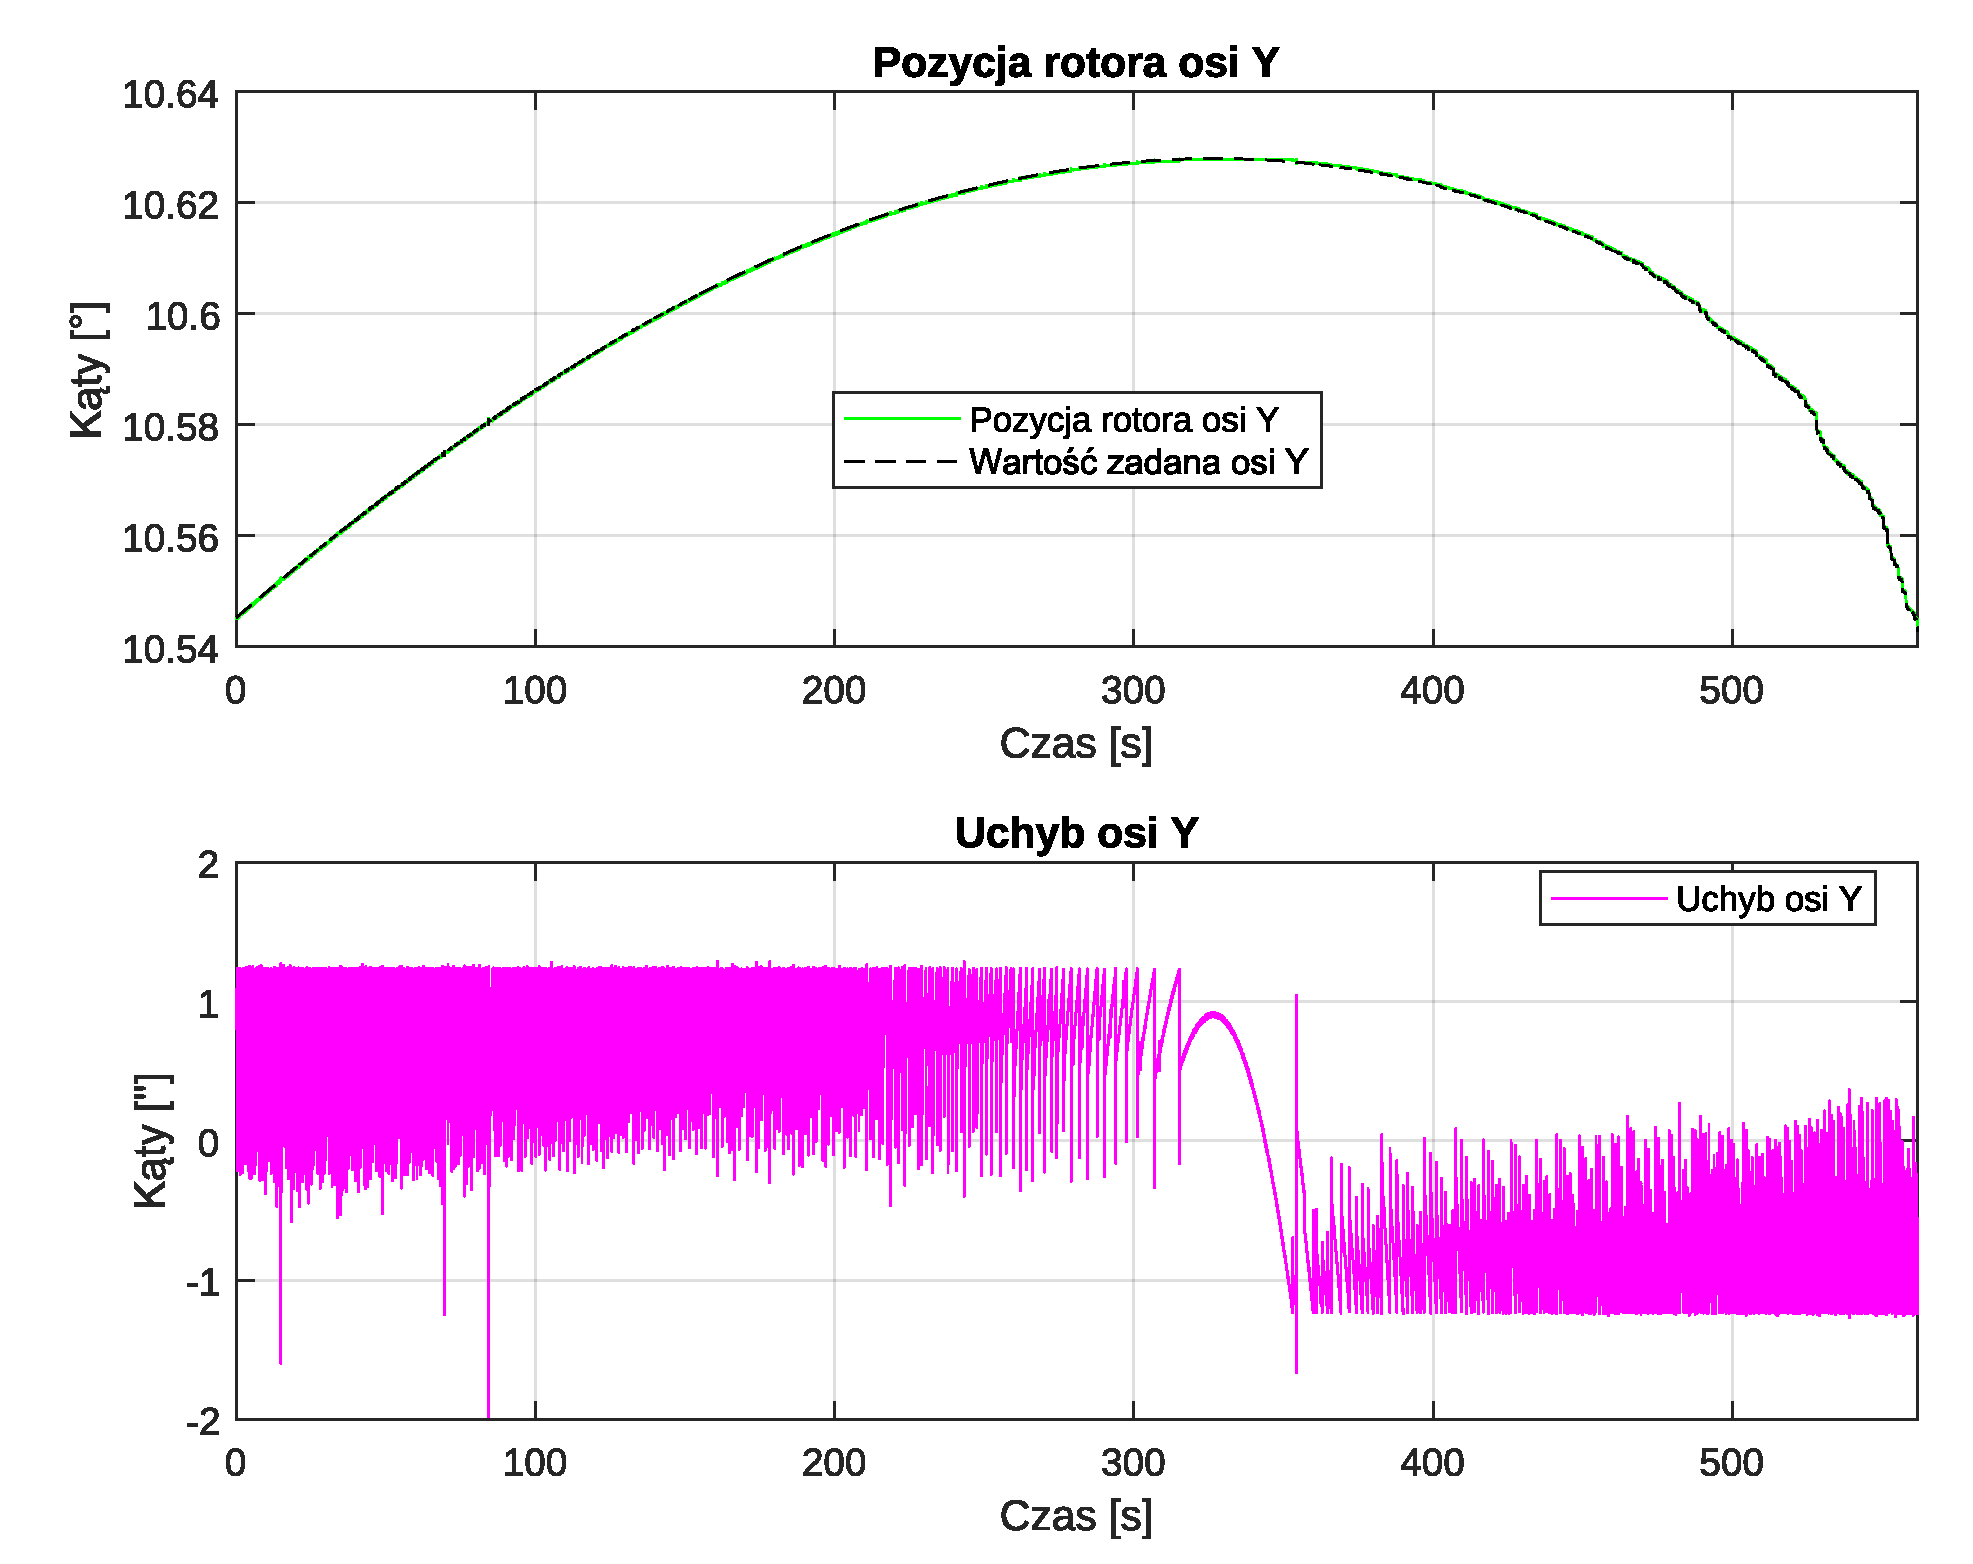
\includegraphics{testy/wykresy_inżynierka/sinus200slongY.pdf}}
    \caption{Przebiegi dla trajektorii sinusoidalnej o okresie 200 sekund na osi Y.}
    \label{fig:Przebiegi dla trajektorii sinusoidalnej o okresie 200 sekund na osi Y.}
\end{figure}

\noindent Dla wszystkich rozważanych trajektorii sinusoidalnych występuje uchyb, który wynika z obecności strefy nieczułości. Dla mniejszych częstotliwości trajektorii sinusoidalnej błąd zawiera się w zakresie zbliżonym do użytej strefy nieczułości (dla bardzo wolnych trajektorii przebieg uchybu praktycznie pozostaje wewnątrz tej strefy - szczególnie to widać na przebiegu \ref{fig:Przebiegi dla trajektorii sinusoidalnej o okresie 200 sekund na osi Y.}). Wynika to z zastosowanej strategii sterowania i nieciągłości pracy regulatora. Dla wyższych częstotliwości układ regulacji przestaje nadążać za trajektorią, co potwierdzają przebiegi \ref{fig:Przebiegi dla trajektorii sinusoidalnej o okresie 1 sekund na osi X.} i \ref{fig:Przebiegi dla trajektorii sinusoidalnej o okresie 1 sekund na osi Y.}. Uchyb dla przebiegów na osi X i Y jest niesymetryczny z powodu cechy konstrukcyjnej.


% Przy różnych częstotliwościach błąd występuje stale, co wynika z cyklicznego generowania sinusa przez mikroprocesor. Po prostu przy zmniejszeniu częstotliwości błąd utrzymuje się stale przez co te wykresy mają większą plamę jakby (analogicznie przy większych). Przy odpowiednio bardzo małej częstotliwości i przybliżeniu punktu odgięcia trajektorii sinusoidalnej widać jak trajektoria próbuje nadążyć i z rachunku referencyjna minus zadana uchyb zmienia wartość na przeciwną, stworzy się taka histereza wtedy co mówił Pazderski jakby ją przyspieszyć wiesz ocb. Po uchybie to widać, zacznie się zmieniać w histerezowo tak jakby w takm kwadracie, w momencie przełączeń zmieni wartość ta histereza. Przy odpowiednio dużych częstotliwościach z kolei układ przestaje nadążać za trajektorią co widać dla wykresu sinus1s. Uchyb już jest dosyć pokaźny. Ja bym powiedział że to ze względu na to jak często odbieramy dane przez spi i , zmiana tych parametrów może nam wpłynąć na precyzję śledzenia, ale obciążymy płytkę w ten sposób bardziej (pole do jakiś tam tych ulepszeń, można to sprawdzić, można to dać do rzeczy jako rozwinięcie pracy, czyli sprawdzenie punktów granicznych). Na moje to nie jest gubienie kroków, bo gubienie kroków to te wartości by musiały przeskakiwać na wykresie a tutaj nic nie skacze (jest na tym samym poziomie jak się coś rzeczywiście zmienia). A no i jeszcze warto wspomnieć o tym, że odkształcający się wykres uchybu w osi y wynika z wady konstrukcyjnej. Ten błąd nie będzie symetrycznie wyglądał, bo jak się wysuwa oś X to Y się napina strasznie i wykres się odkształca. Tam to sprzężenie było przeciwnie więc jak u nas się w X wysuwa to w Y się wsuwa patrząc na wartości, czyli jest git, ta oś Y się napina bo próbuje się skurczyć a że materiał trwały aluminium to nie ma jak i ten błąd jest taki duży w tym momencie na tych wykresach.


\section{Trajektoria prostokątna}
\begin{figure}[H]
    \centering
    \resizebox{12cm}{!}{
    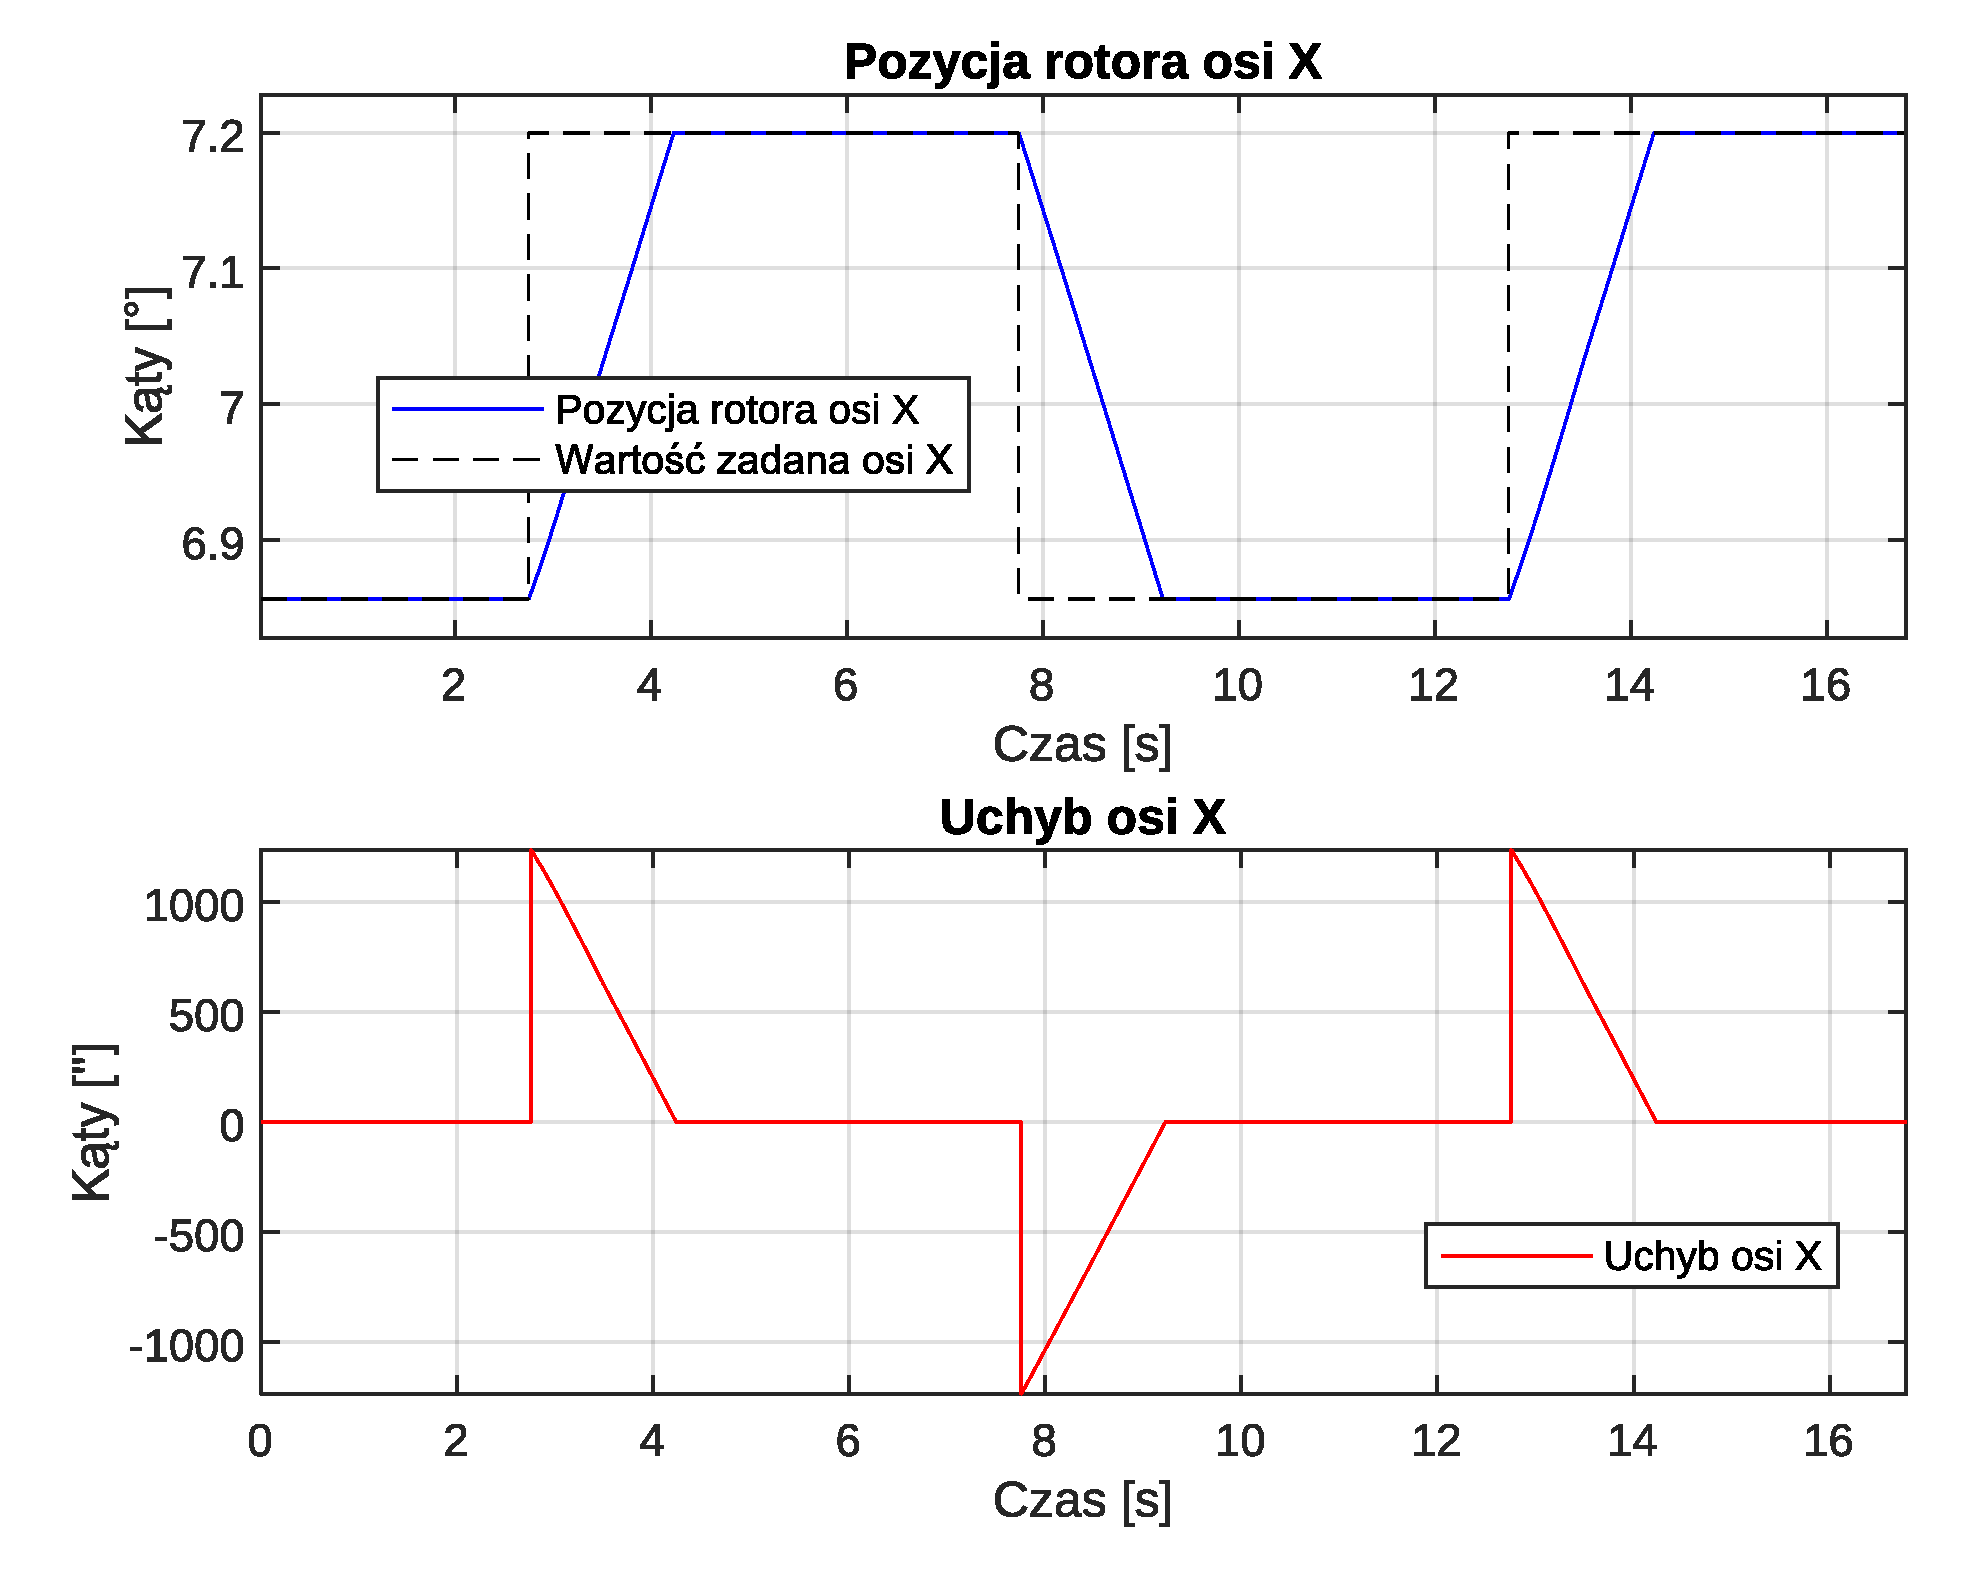
\includegraphics{testy/wykresy_inżynierka/squareX.pdf}}
    \label{fig:schemat blokowy pobierania danych2}
    \caption{Przebiegi dla trajektorii prostokątnej o okresie 10 sekund na osi X.}
\end{figure}

\begin{figure}[H]
    \centering
    \resizebox{12cm}{!}{
    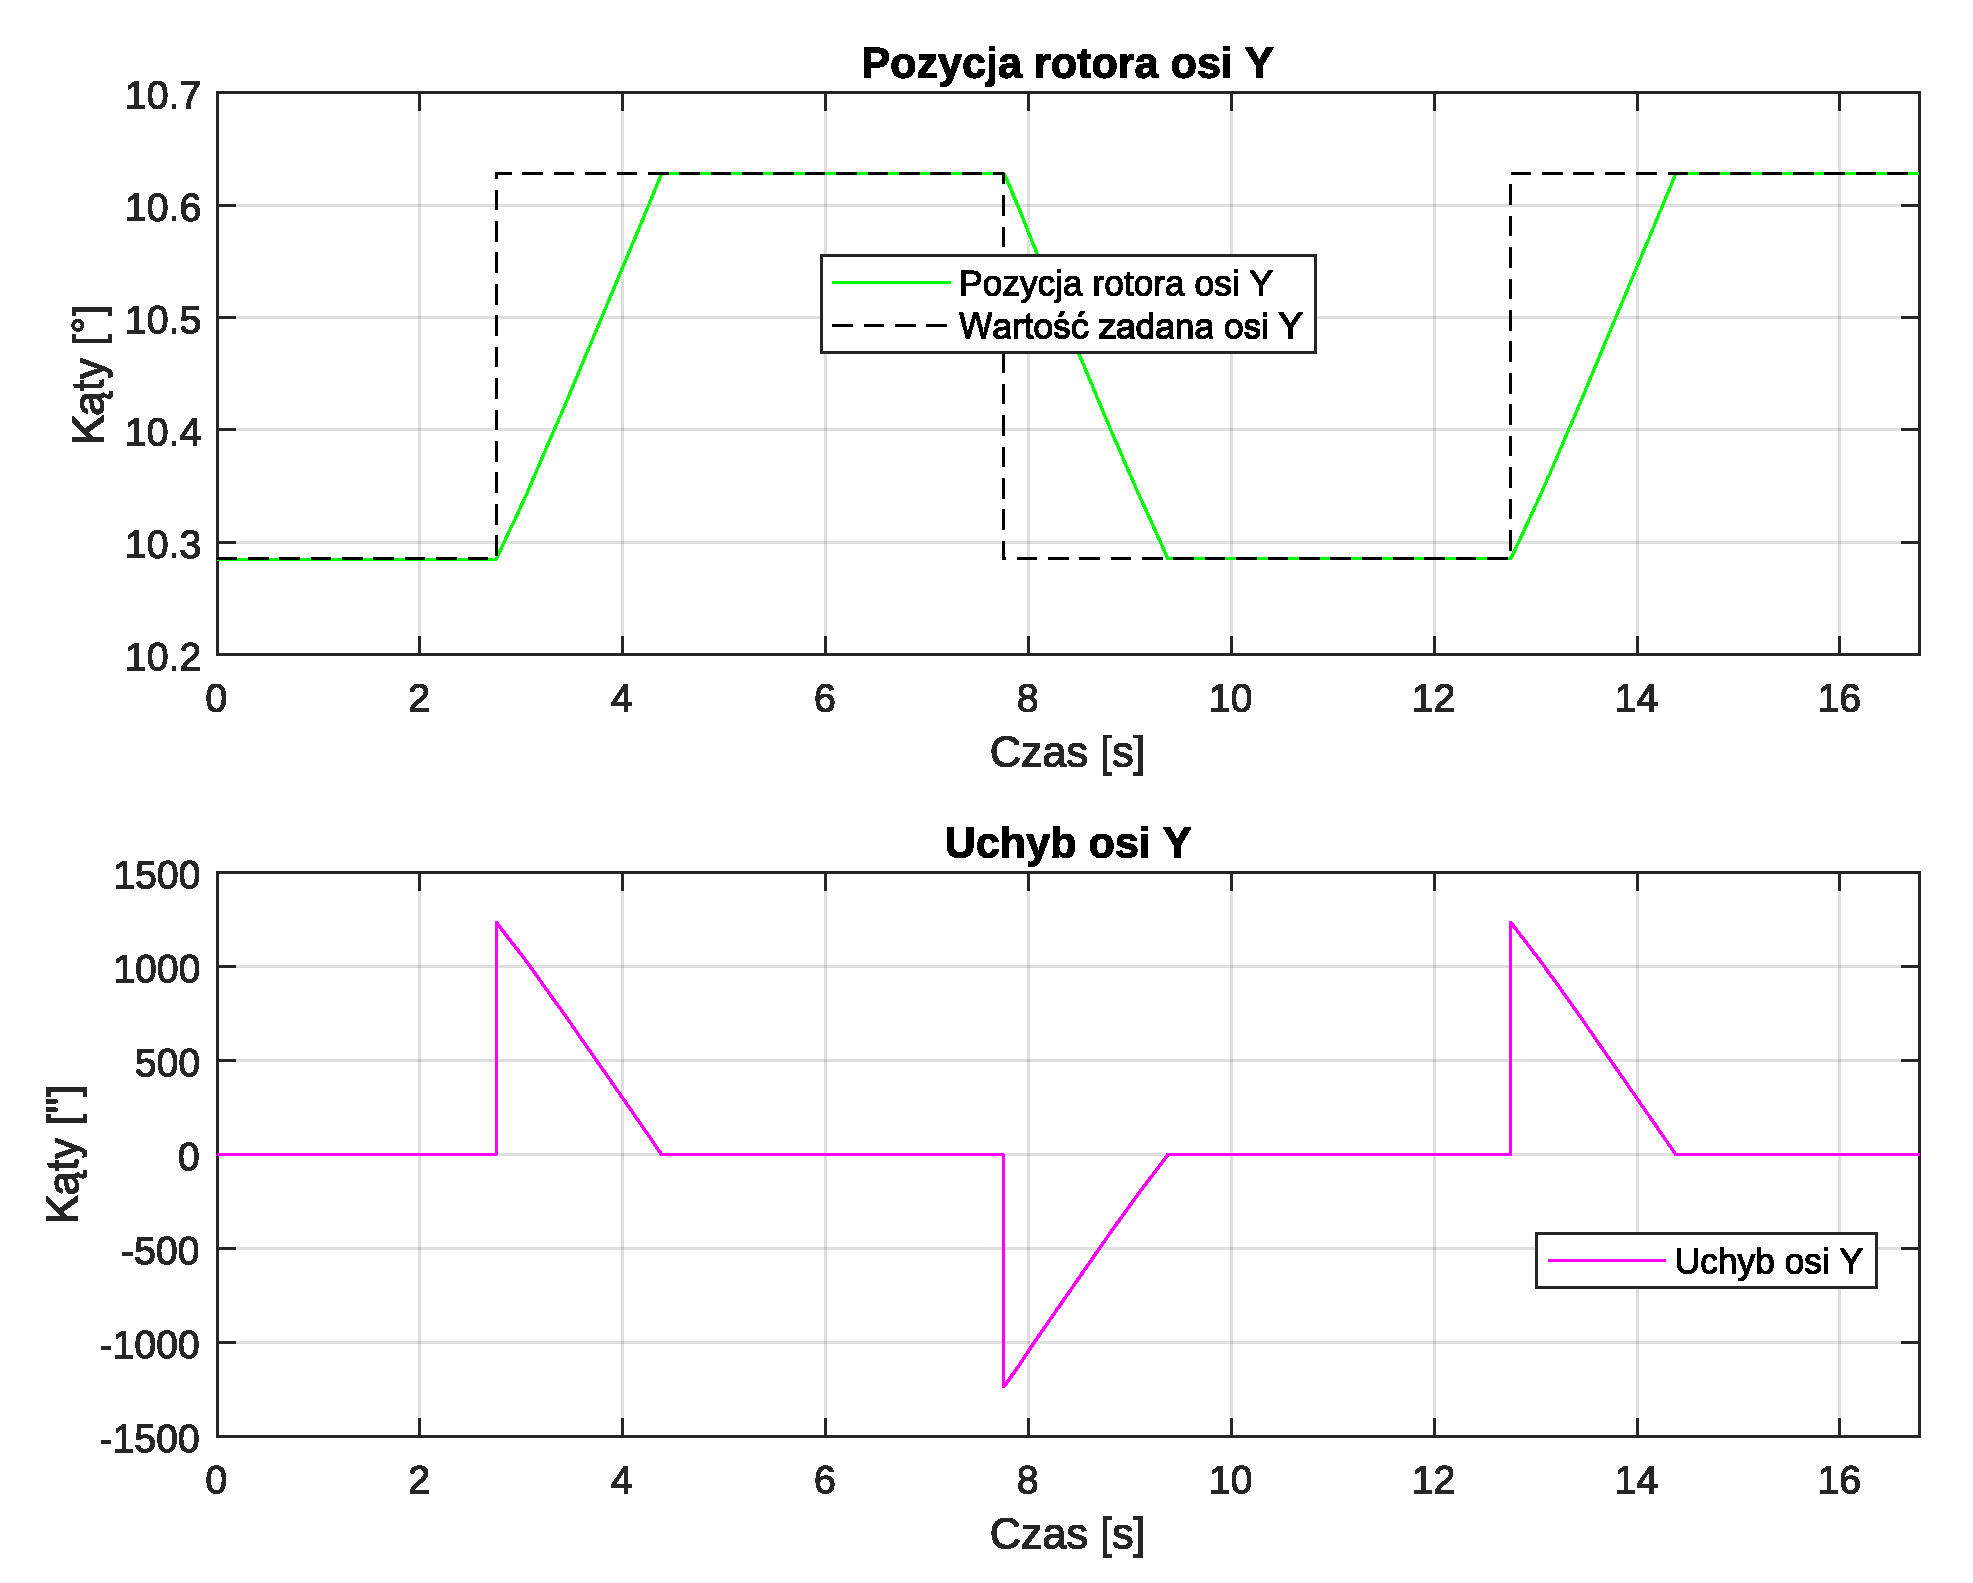
\includegraphics{testy/wykresy_inżynierka/squareY.pdf}}
    \label{fig:schemat blokowy pobierania danych2}
    \caption{Przebiegi dla trajektorii prostokątnej o okresie 10 sekund na osi Y.}
\end{figure}

% W momencie nawrotu, czyli skokowych zmian pozycji, układ dąży do osiągnięcia celu po ponad sekundzie. (nie wiem co tu więcej można powiedzieć). Generalnie jest gicio, działa (tutaj też można wspomnieć, że można się pobawić tymi stałymi czasowymi i przetestować dla jakich częstotliwości zbierania próbek z enkodera i zmienieniu martwej strefy zmieni się stała czasowa i czy to ma wpływ wgl, tutaj imo odległość gra rolę, bo gdyby ten punkt miał być dalej to ten wykres by dalej próbował nadążyć, można da porównania zrobić taki i opisać)  
Zastosowana metoda sterowania silnikiem krokowym powoduje w przybliżeniu stałą prędkość obrotu osi. Podczas dynamicznych zmian wartości zadanej pozycja nie osiąga natychmiast nowej wartości, lecz zmienia się liniowo, to jest silnik musi wykonać odpowiednią liczbę kroków. 

\section{Badanie wpływu większej częstotliwości sterowania pracą silników}

\vspace{1cm}

\begin{center}
    \textbf{Synchronizacja momentu odczytywania danych z sygnałami podawanymi na wejście CLK}
\end{center}

\begin{figure}[H]
    \centering
    \resizebox{16cm}{!}{
    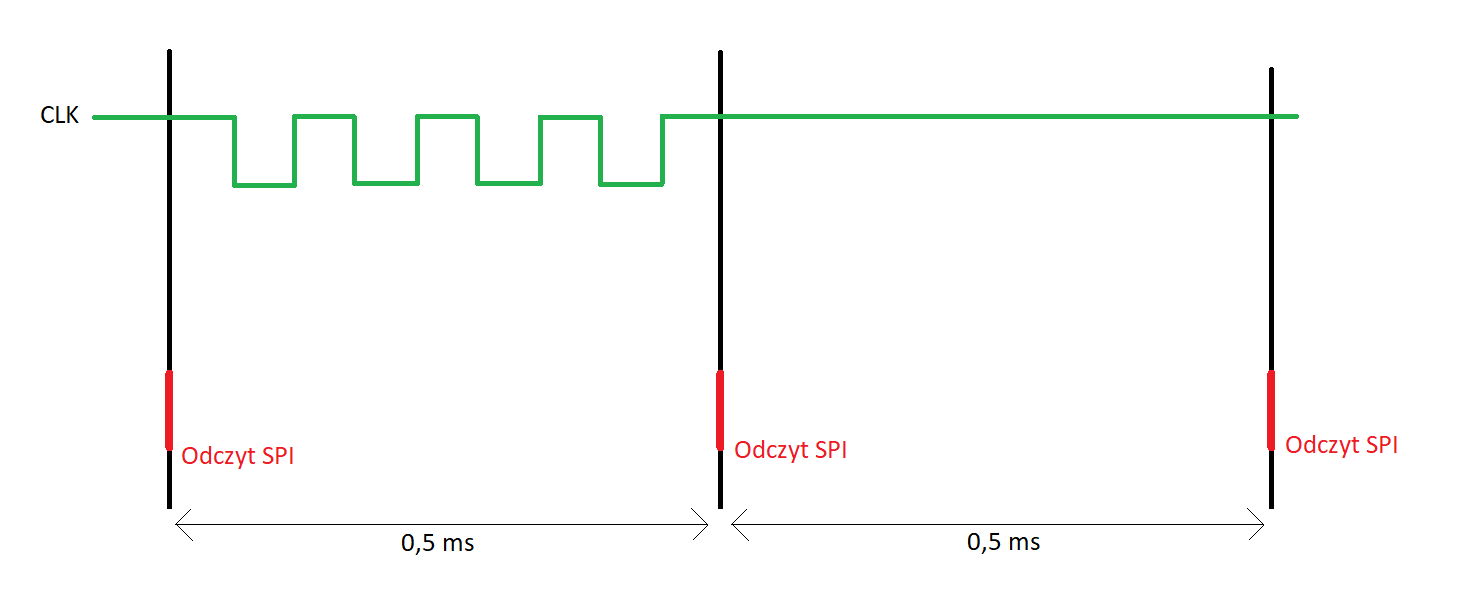
\includegraphics{pictures/image.png}}
    \caption{Sterowanie sygnałem na wejściu CLK.}
    \label{fig:Sterowanie sygnałem na wejściu CLK}
\end{figure}

\noindent W tym eksperymencie pozostawiono częstotliwość próbkowania 2kHz, zmieniano jednak częstotliwość sygnału zegarowego sterującego prędkością przełączania silnika za pomocą niezależnego timera. Powoduje to wprowadzenie pewnego asynchronizmu w sterowaniu, ponieważ tylko niektóry cykl zegara generowany jest na podstawie bieżącej pozycji. Graficzna reprezentacja całego procesu została przedstawiona na rysunku \ref{fig:Sterowanie sygnałem na wejściu CLK}. Tryb synchroniczny nie był implementowany dla częstotliwości próbkowania powyżej 2kHz z uwagi na ograniczone zasoby obliczeniowe mikrokontolera.

\begin{figure}[H]
    \centering
    \resizebox{12cm}{!}{
    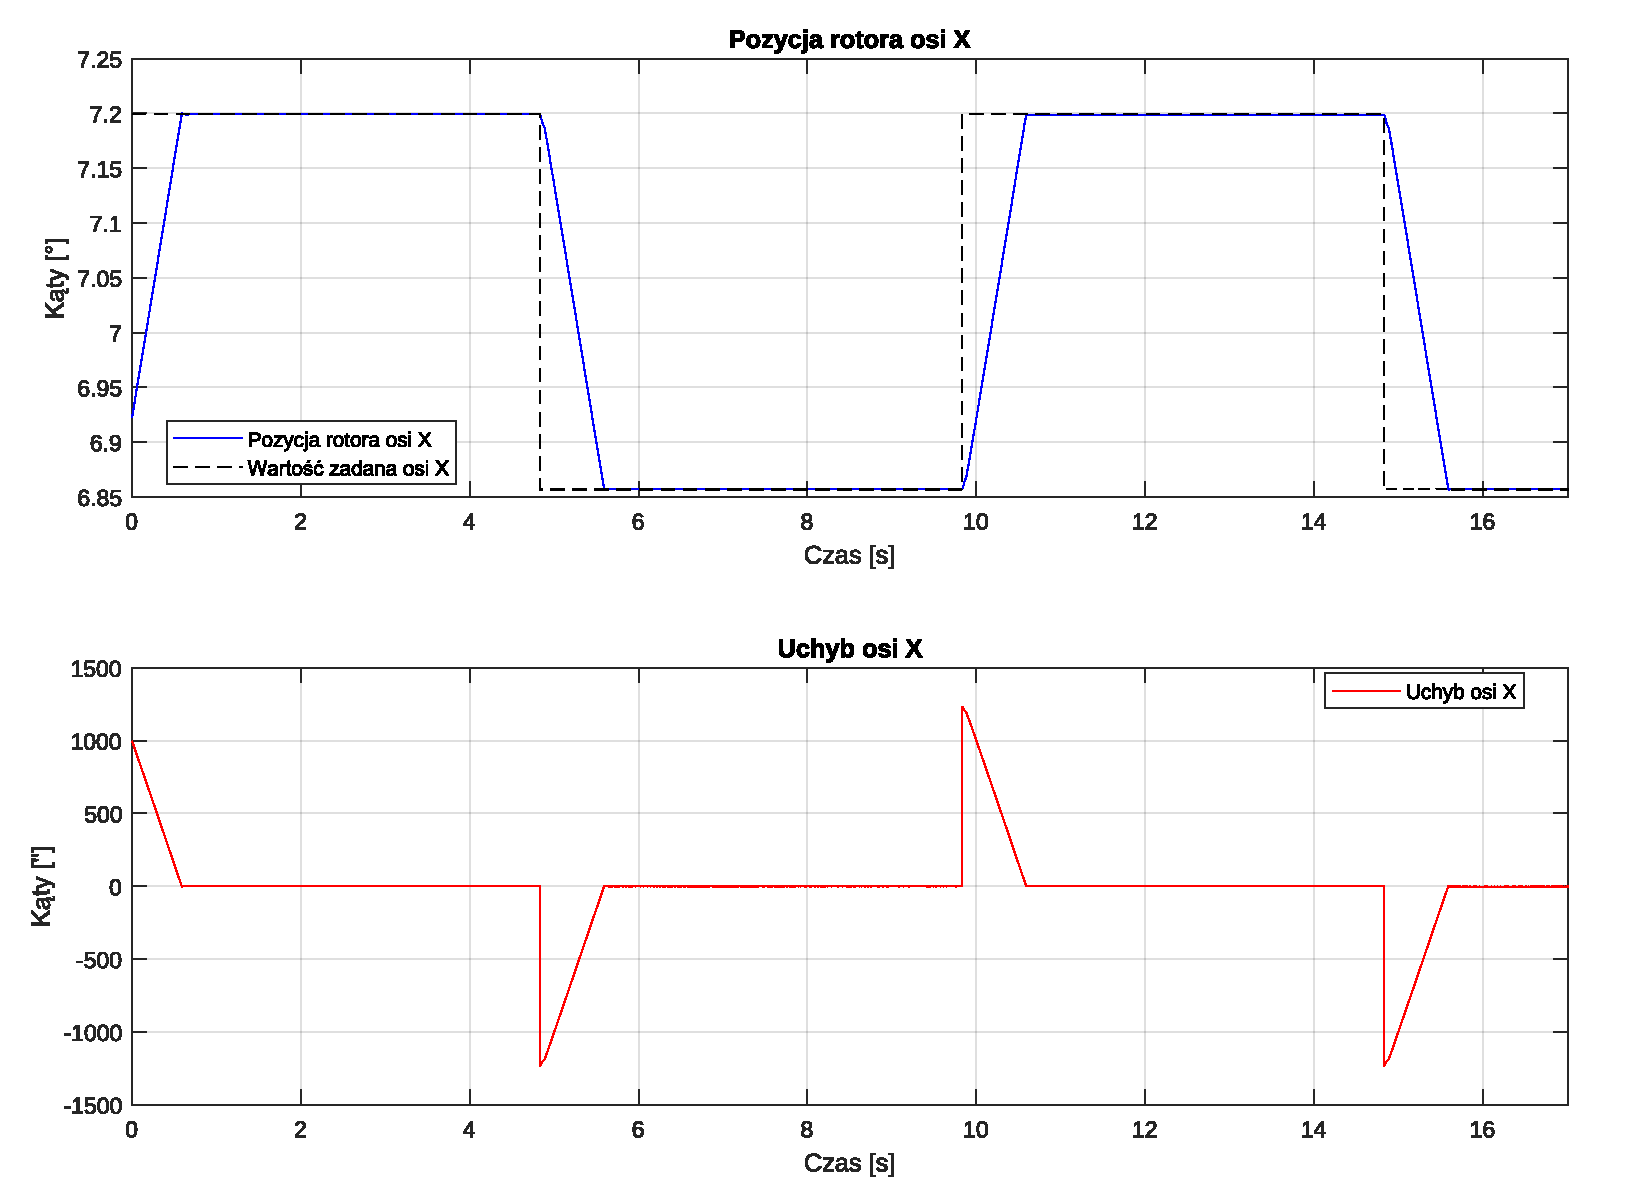
\includegraphics{testy/wykresy_inżynierka/4kY.pdf}}
    \caption{Przebiegi dla sterowania z częstotliwością 4000 Hz na osi X.}
    \label{fig:schemat blokowy pobierania danych2}
\end{figure}


\begin{figure}[H]
    \centering
    \resizebox{12cm}{!}{
    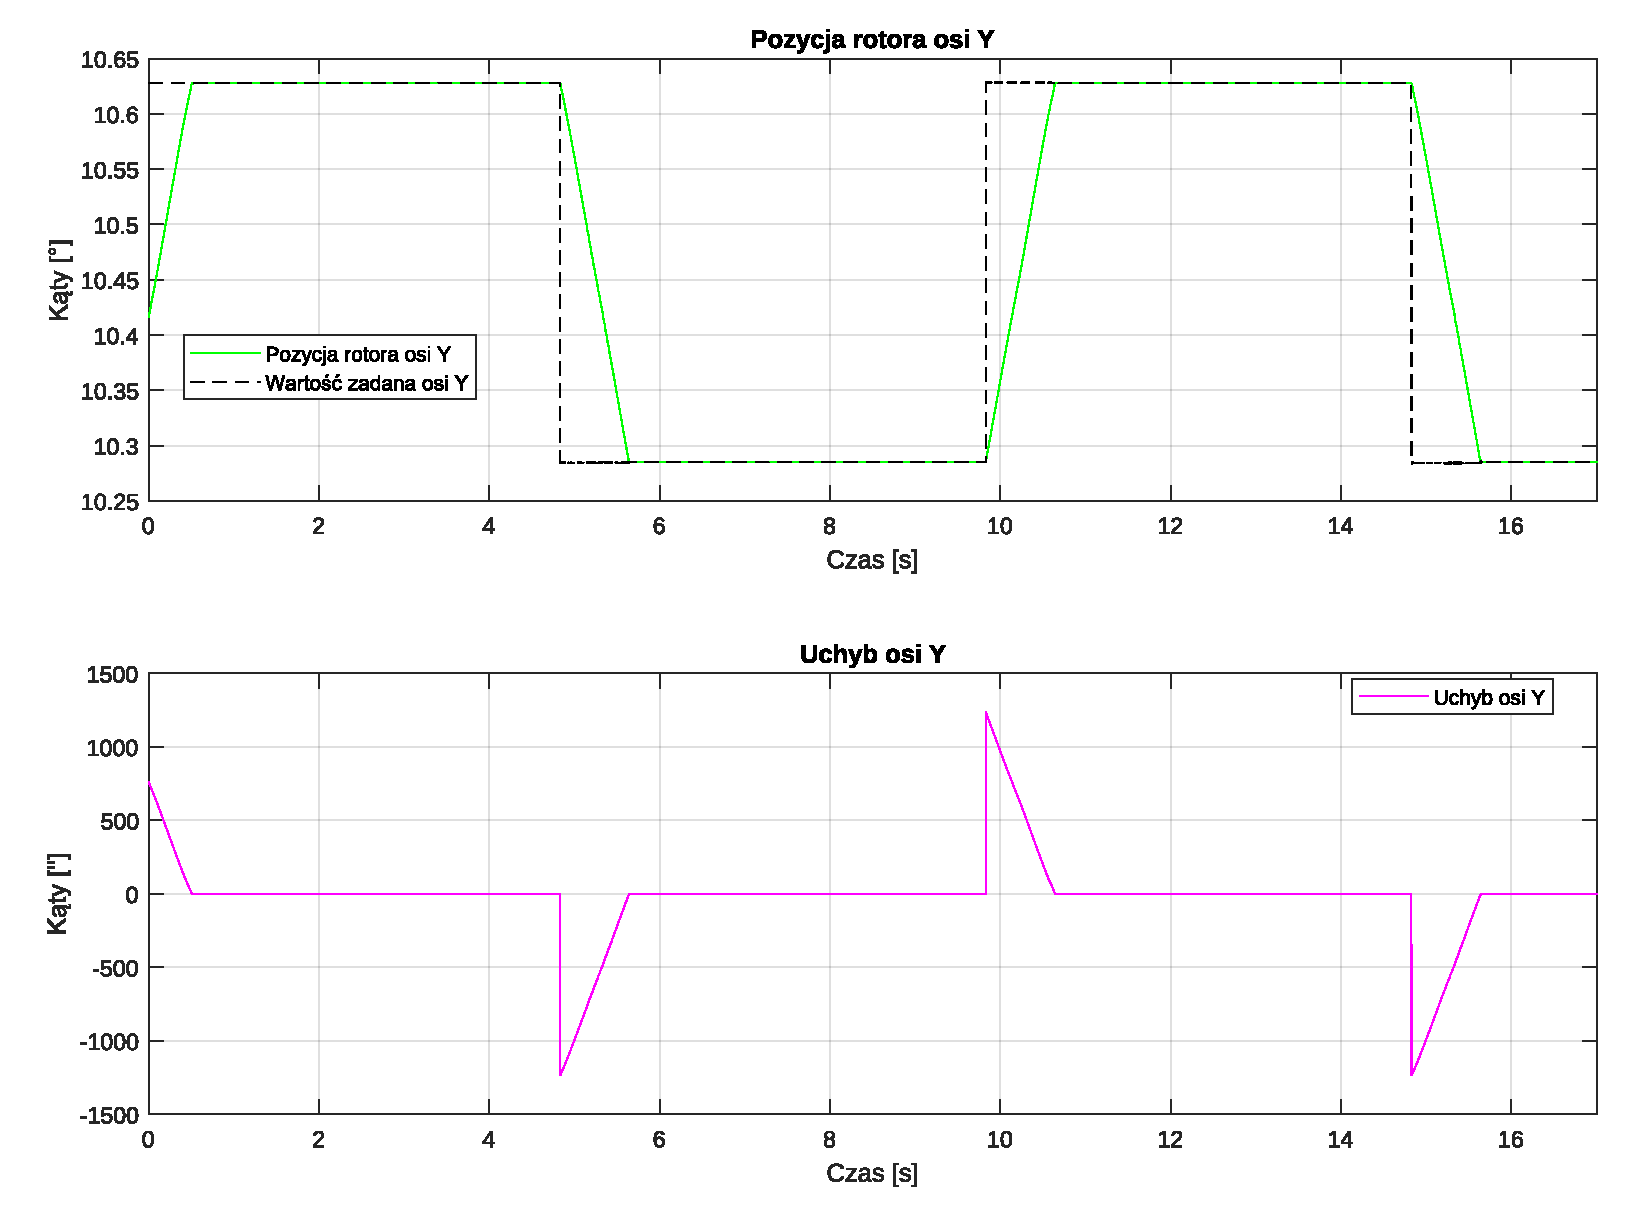
\includegraphics{testy/wykresy_inżynierka/4kX.pdf}}
    \caption{Przebiegi dla sterowania z częstotliwością 4000 Hz na osi Y.}
    \label{fig:schemat blokowy pobierania danych2}
\end{figure}

\begin{figure}[H]
    \centering
    \resizebox{12cm}{!}{
    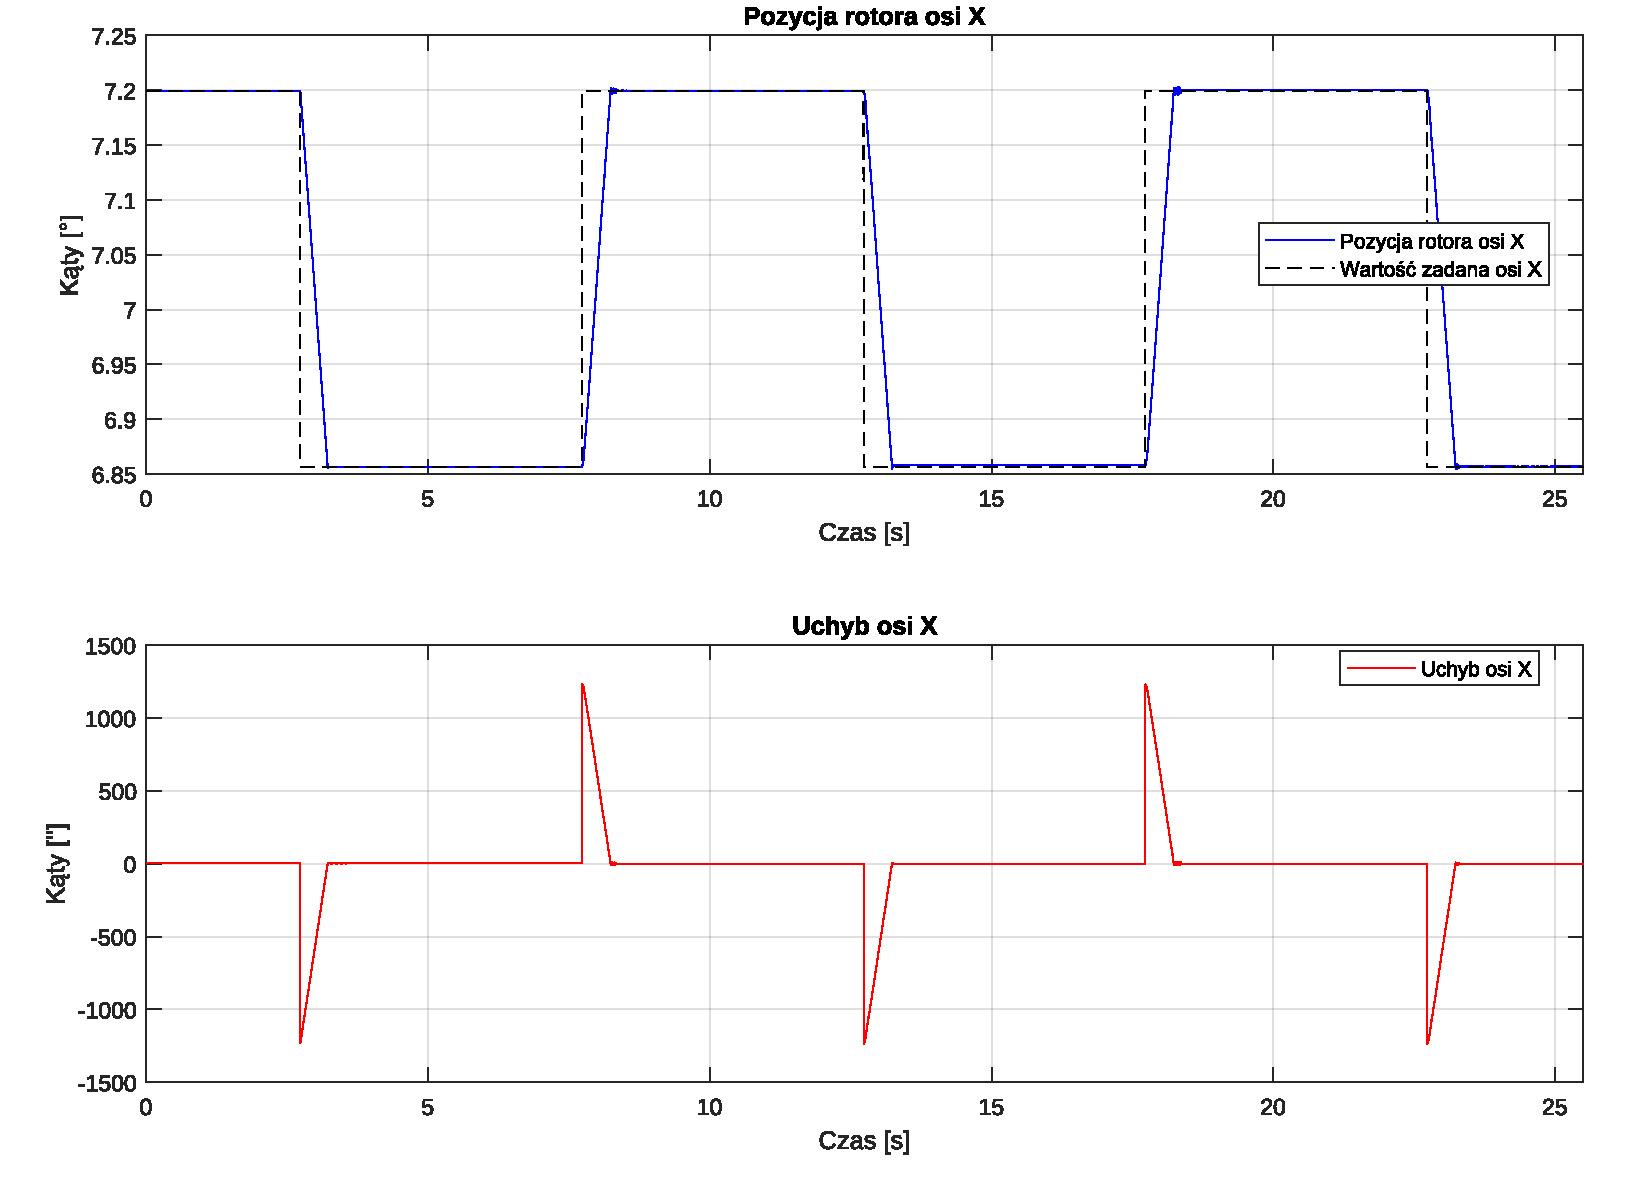
\includegraphics{testy/wykresy_inżynierka/6kX.pdf}}
    \caption{Przebiegi dla sterowania z częstotliwością 6000 Hz na osi X.}
    \label{fig:schemat blokowy pobierania danych2}
\end{figure}


\begin{figure}[H]
    \centering
    \resizebox{12cm}{!}{
    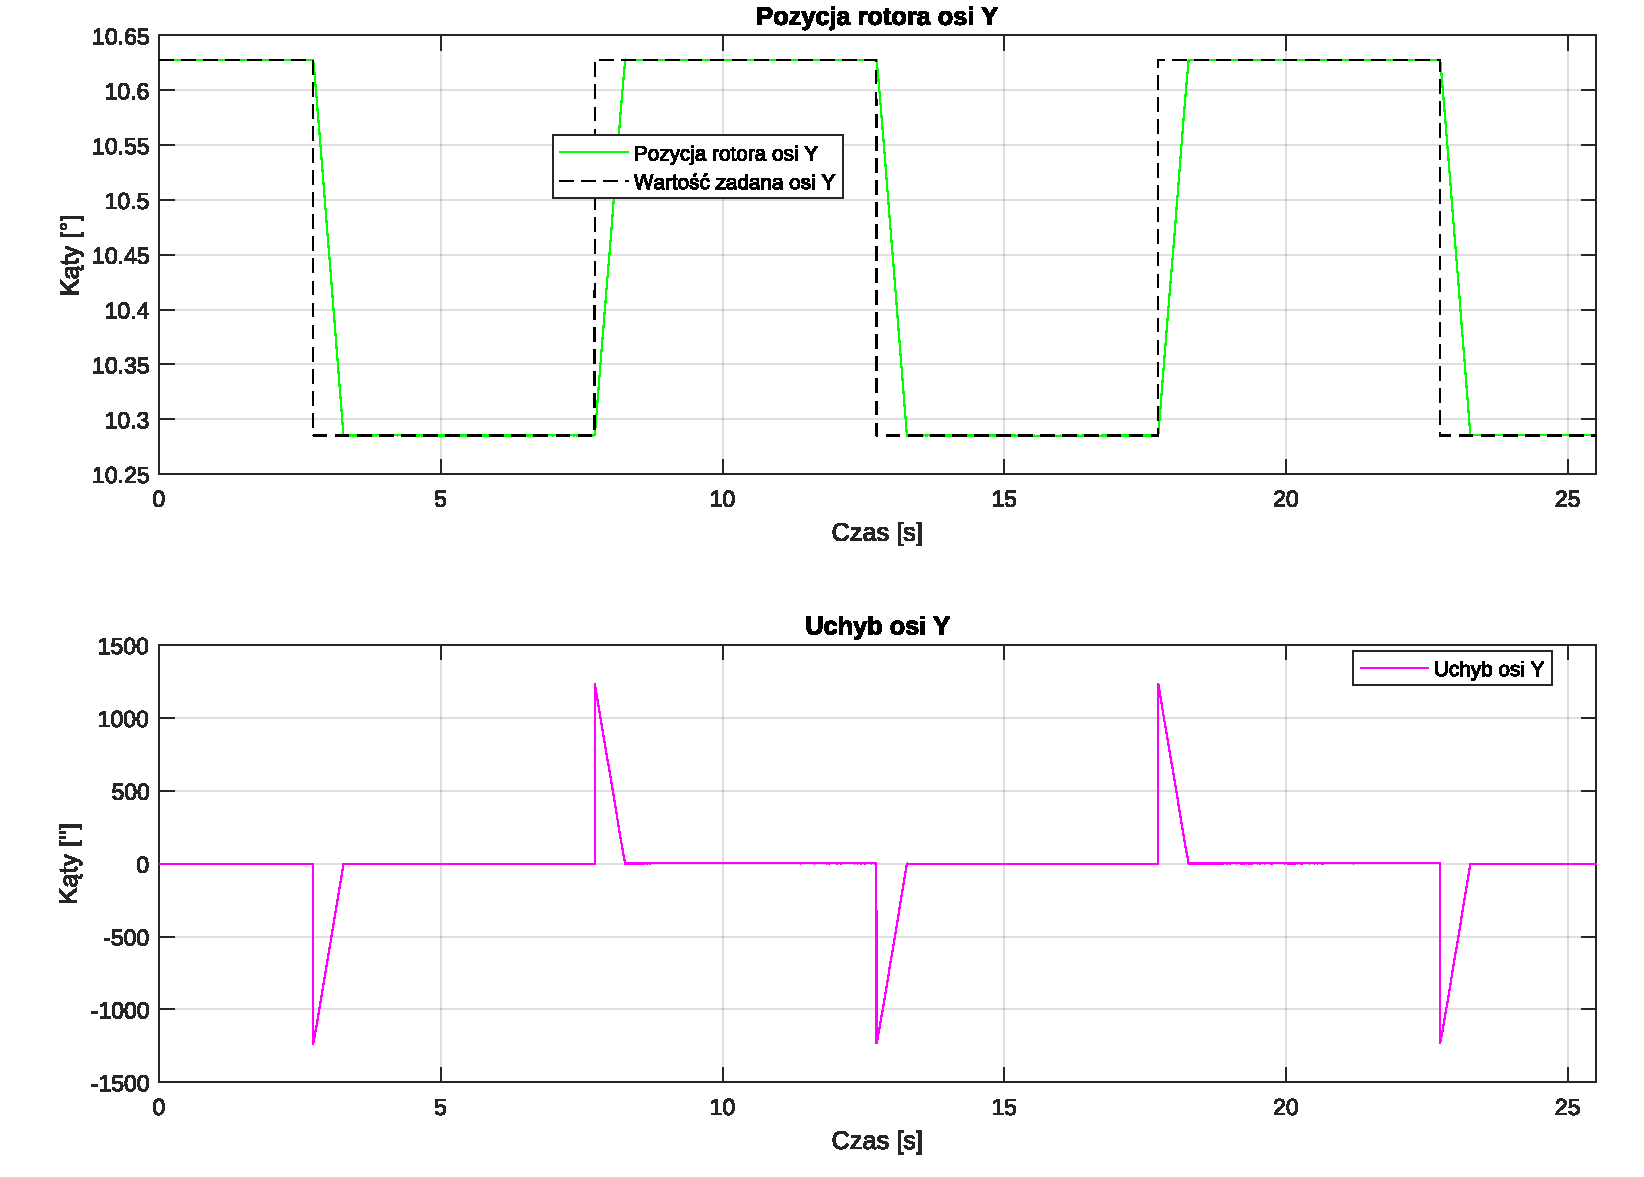
\includegraphics{testy/wykresy_inżynierka/6kY.pdf}}
    \caption{Przebiegi dla sterowania z częstotliwością 6000 Hz na osi Y.}
    \label{fig:schemat blokowy pobierania danych2}
\end{figure}


\begin{figure}[H]
    \centering
    \resizebox{12cm}{!}{
    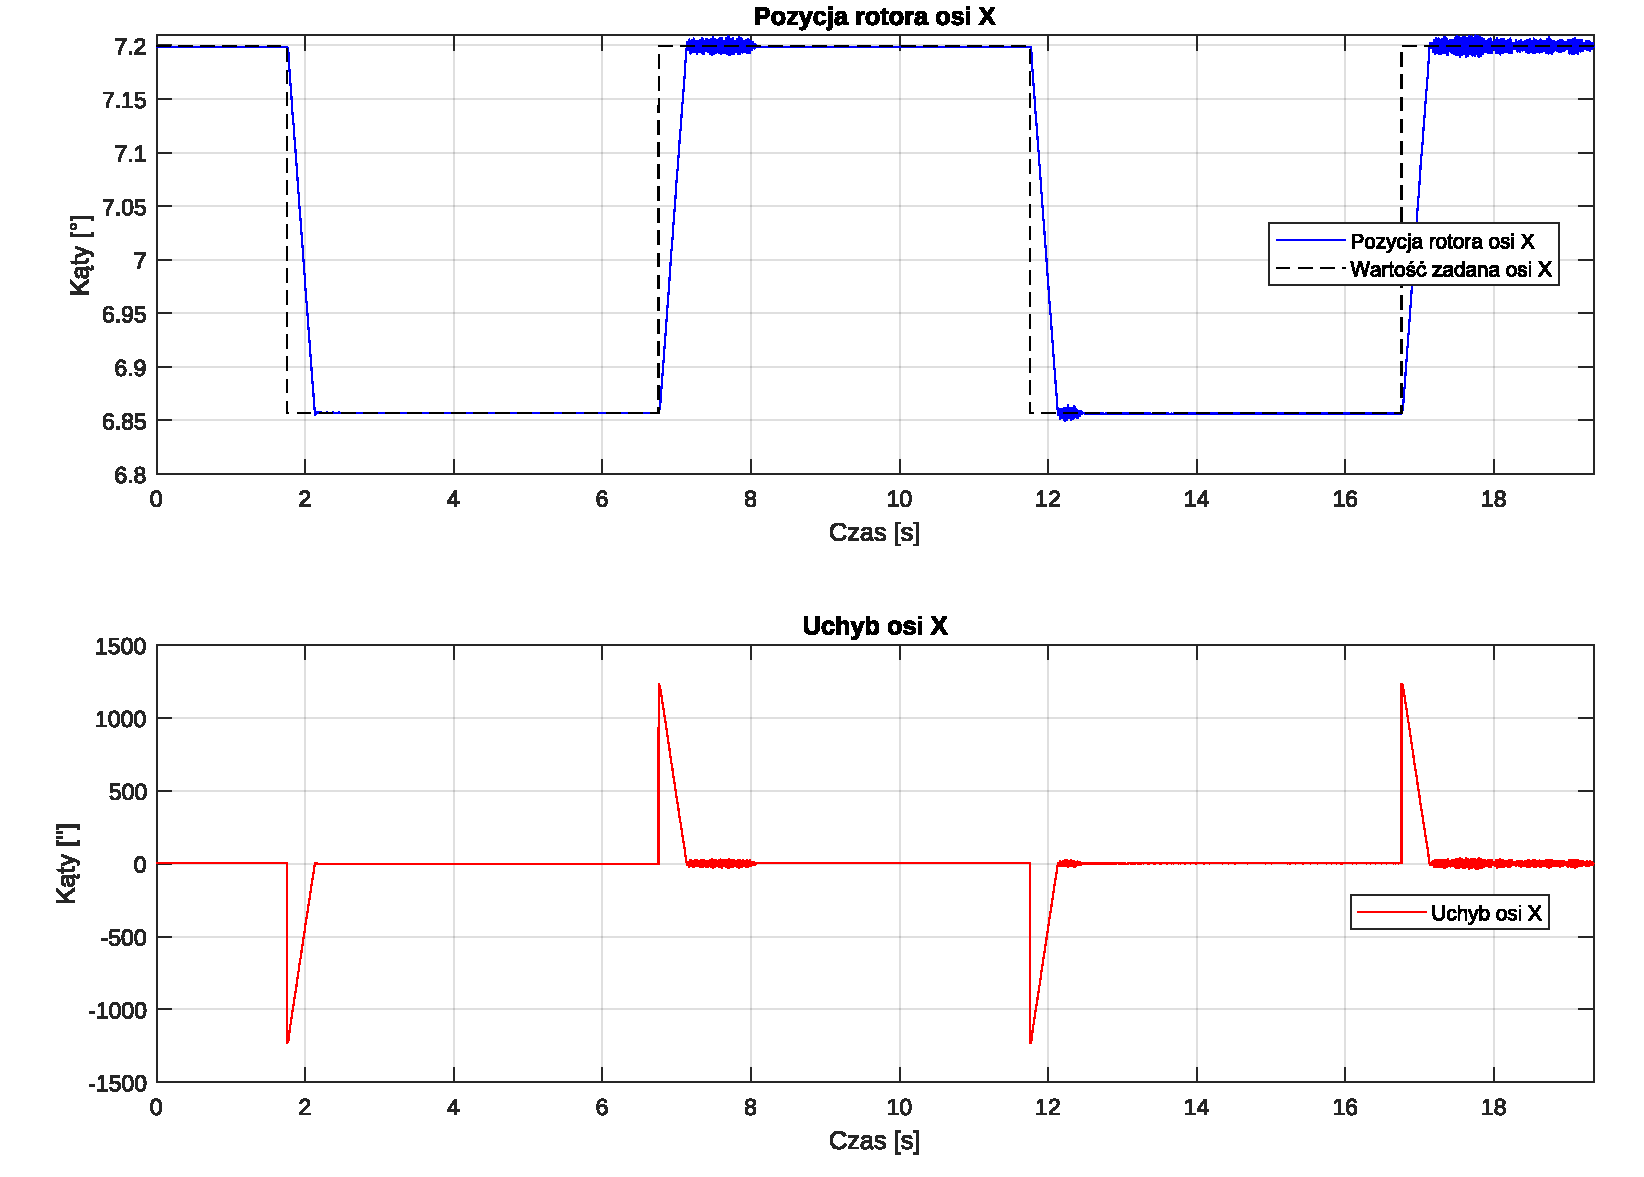
\includegraphics{testy/wykresy_inżynierka/8kX.pdf}}
    \caption{Przebiegi dla sterowania z częstotliwością 8000 Hz na osi X.}
    \label{fig:schemat blokowy pobierania danych2}
\end{figure}


\begin{figure}[H]
    \centering
    \resizebox{12cm}{!}{
    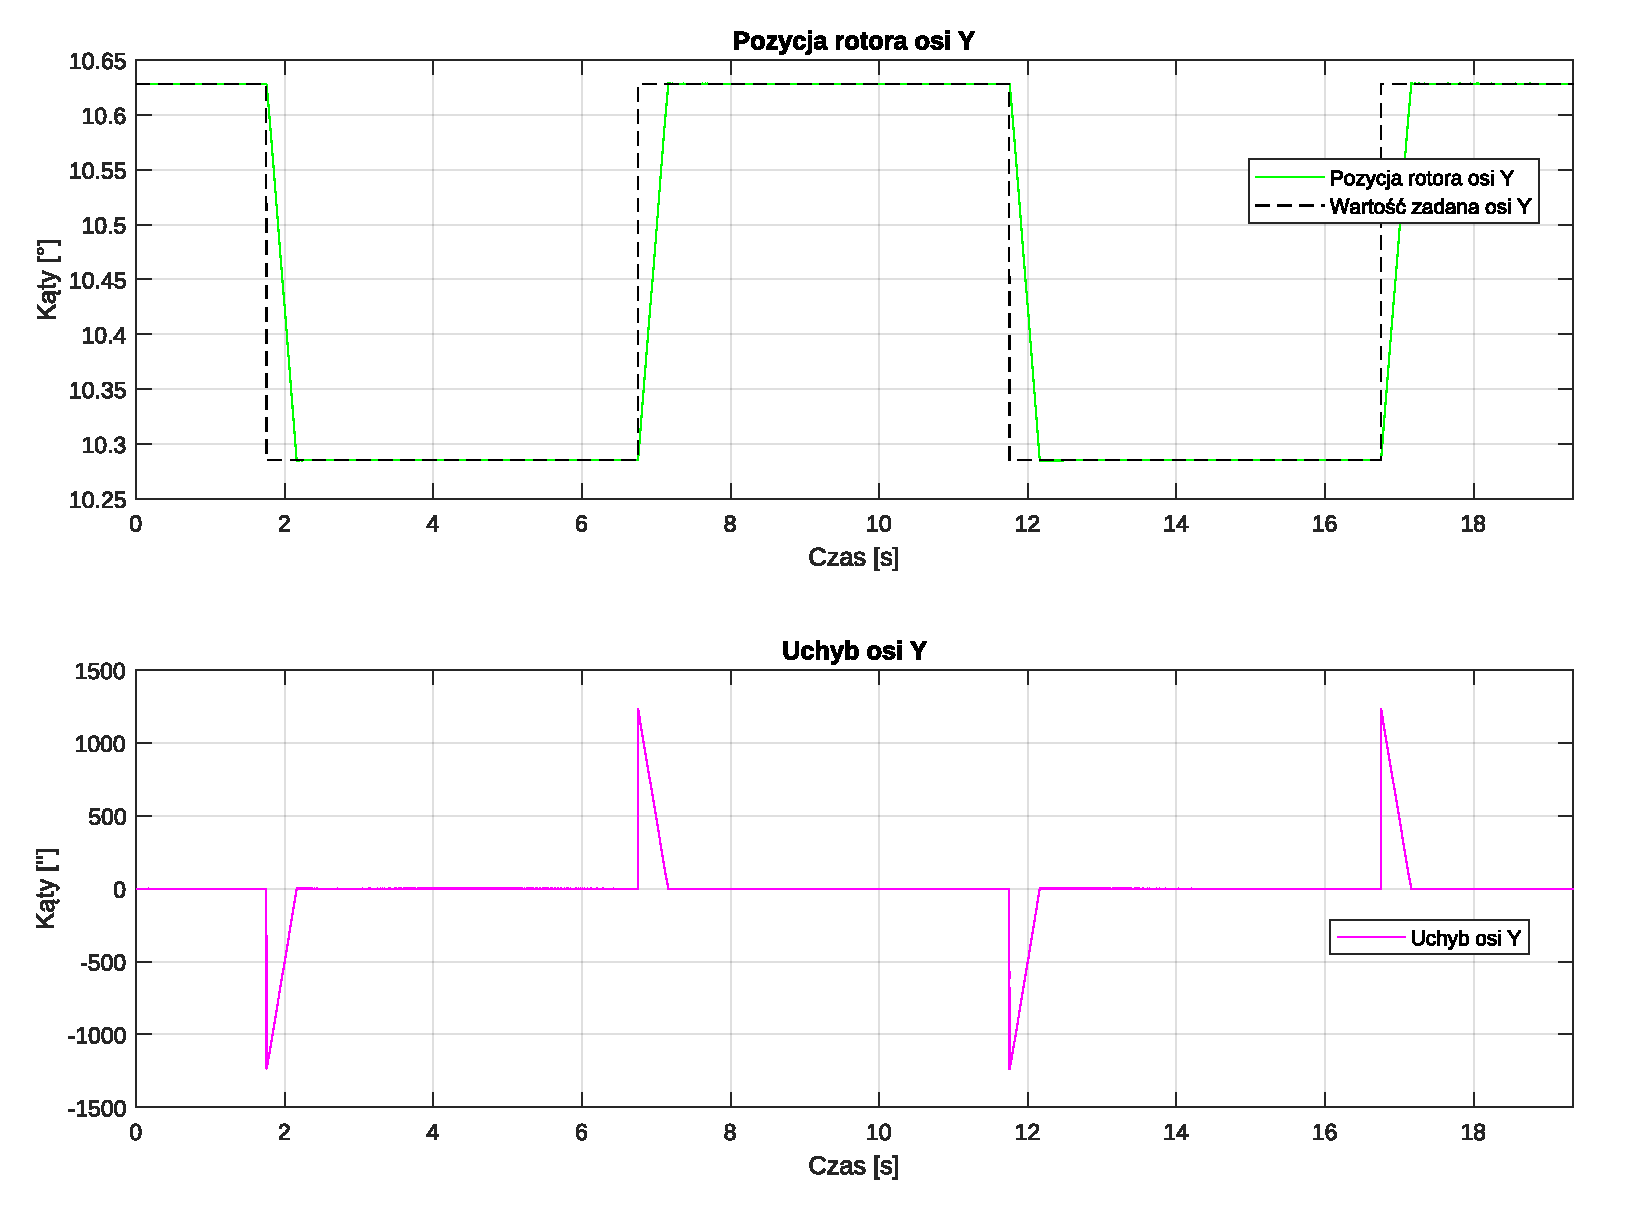
\includegraphics{testy/wykresy_inżynierka/8kY.pdf}}
    \caption{Przebiegi dla sterowania z częstotliwością 8000 Hz na osi Y.}
    \label{fig:schemat blokowy pobierania danych2}
\end{figure}


\begin{figure}[H]
    \centering
    \resizebox{12cm}{!}{
    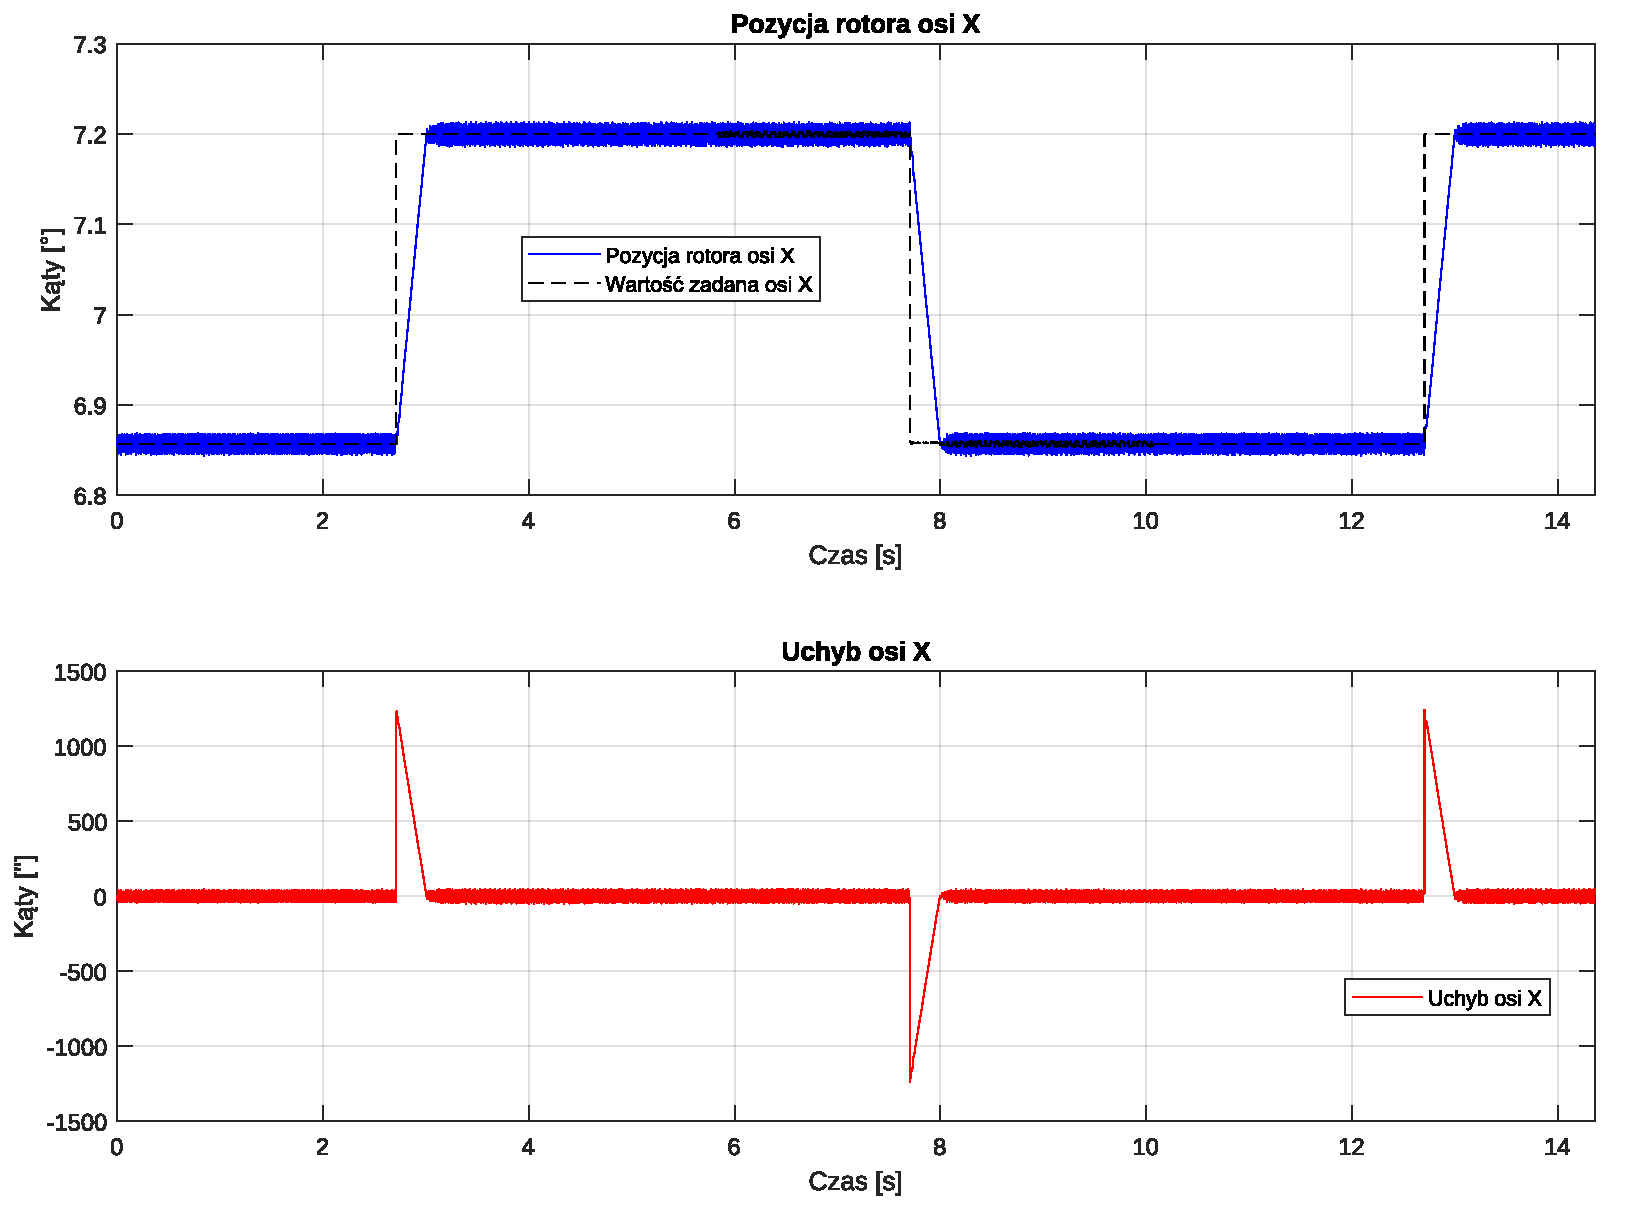
\includegraphics{testy/wykresy_inżynierka/10kX.pdf}}
    \caption{Przebiegi dla sterowania z częstotliwością 10000 Hz na osi X.}
    \label{fig:schemat blokowy pobierania danych2}
\end{figure}


\begin{figure}[H]
    \centering
    \resizebox{12cm}{!}{
    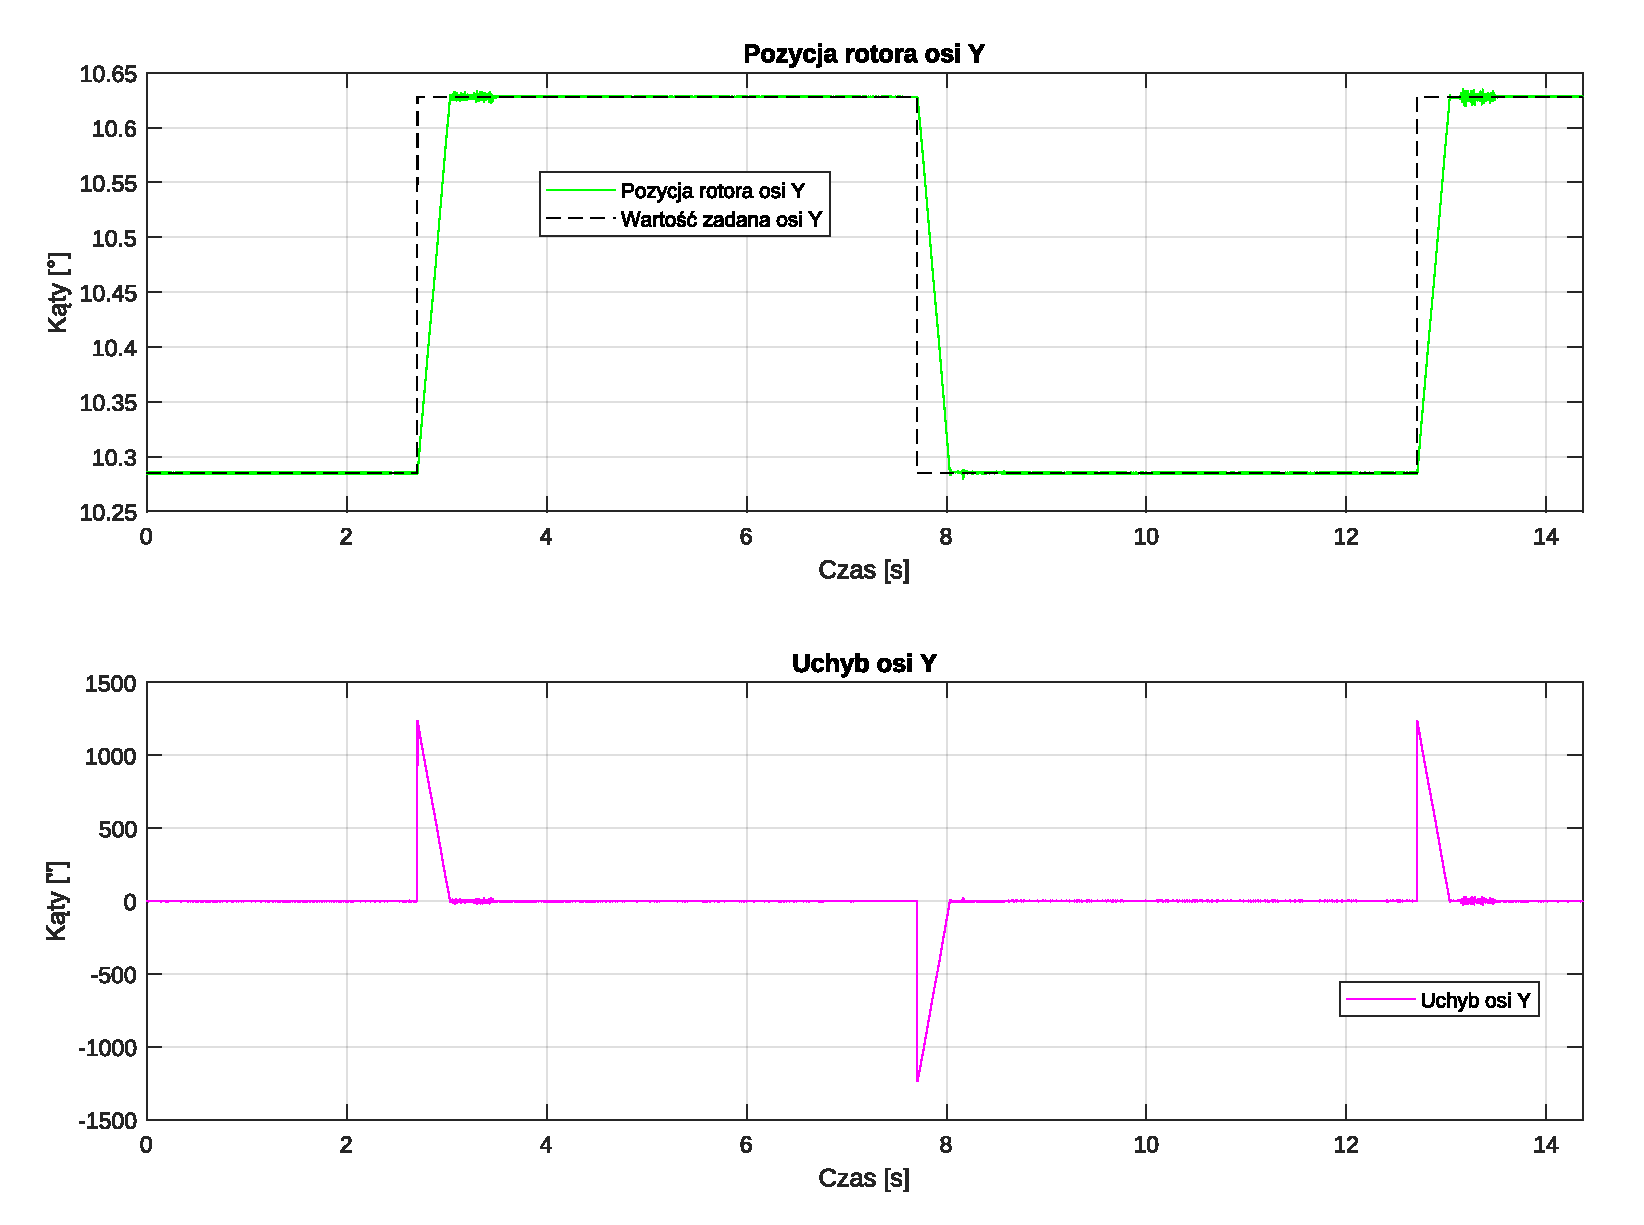
\includegraphics{testy/wykresy_inżynierka/10kY.pdf}}
    \caption{Przebiegi dla sterowania z częstotliwością 10000 Hz na osi Y.}
    \label{fig:schemat blokowy pobierania danych2}
\end{figure}


\begin{figure}[H]
    \centering
    \resizebox{12cm}{!}{
    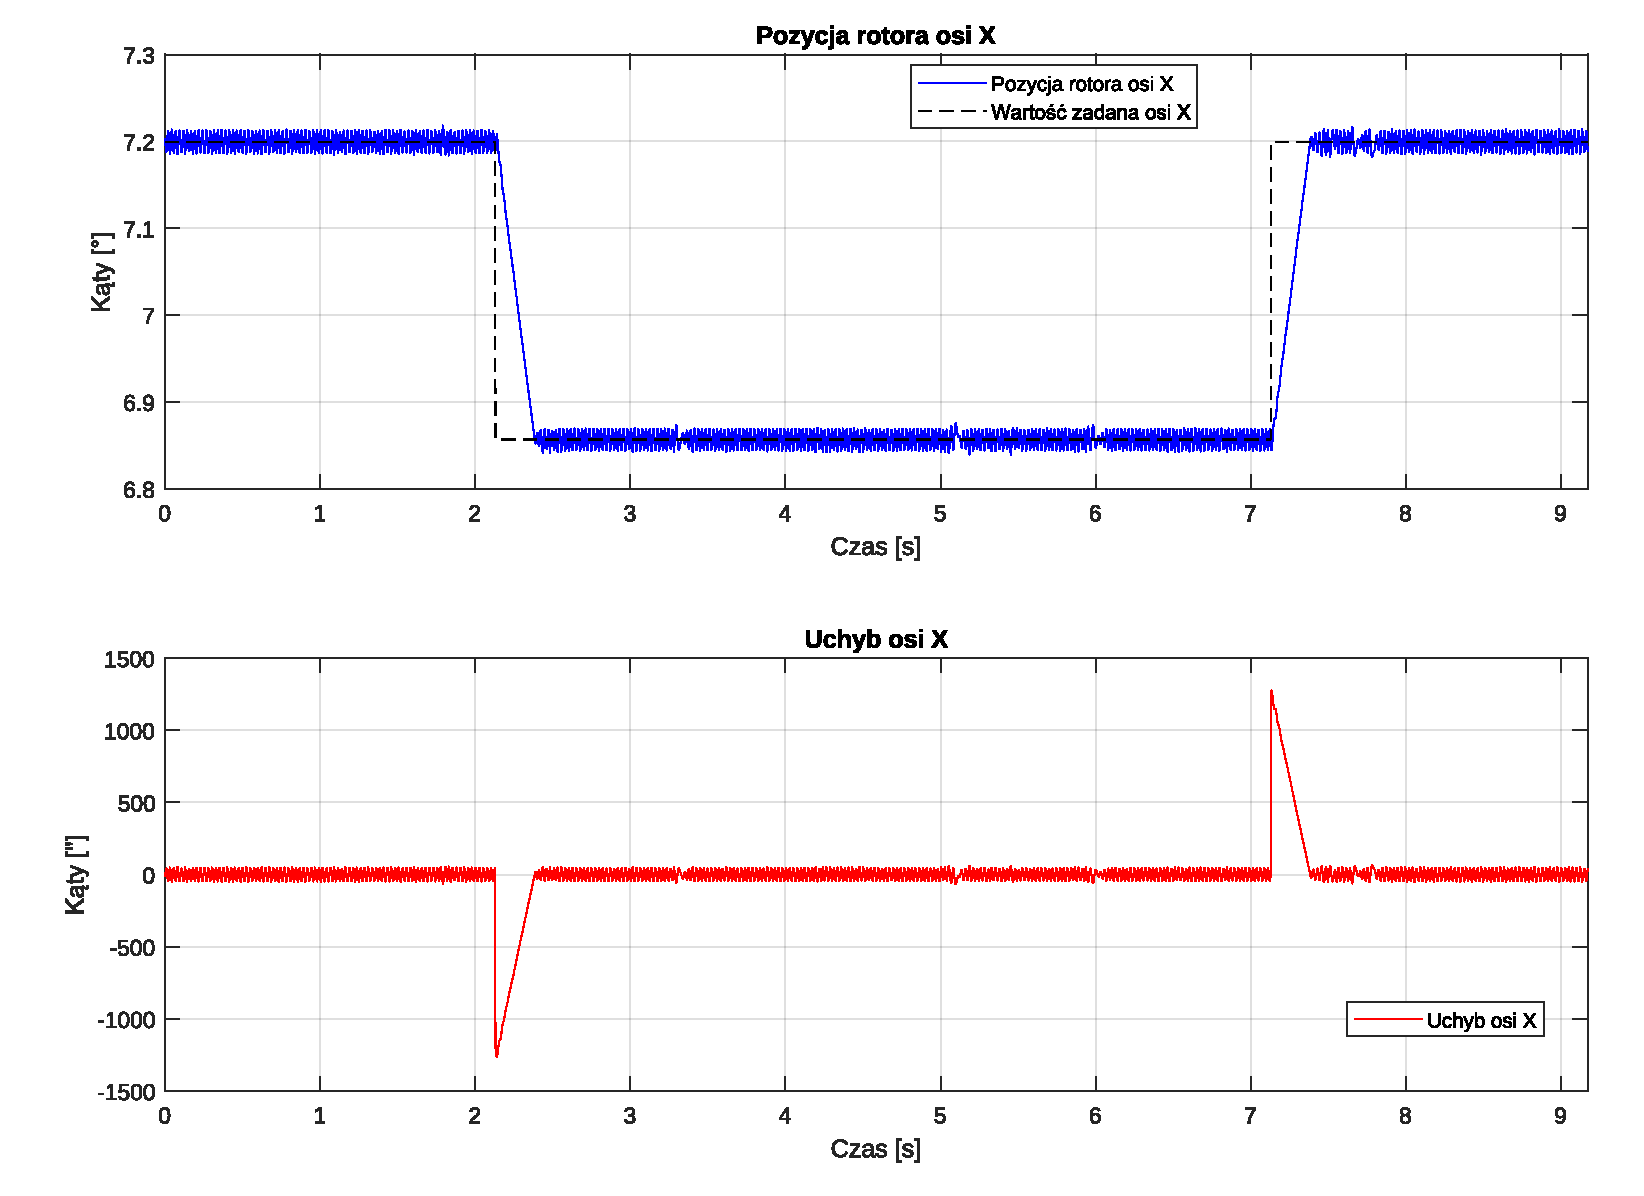
\includegraphics{testy/wykresy_inżynierka/12kX.pdf}}
    \caption{Przebiegi dla sterowania z częstotliwością 12000 Hz na osi X.}
    \label{fig:schemat blokowy pobierania danych2}
\end{figure}


\begin{figure}[H]
    \centering
    \resizebox{12cm}{!}{
    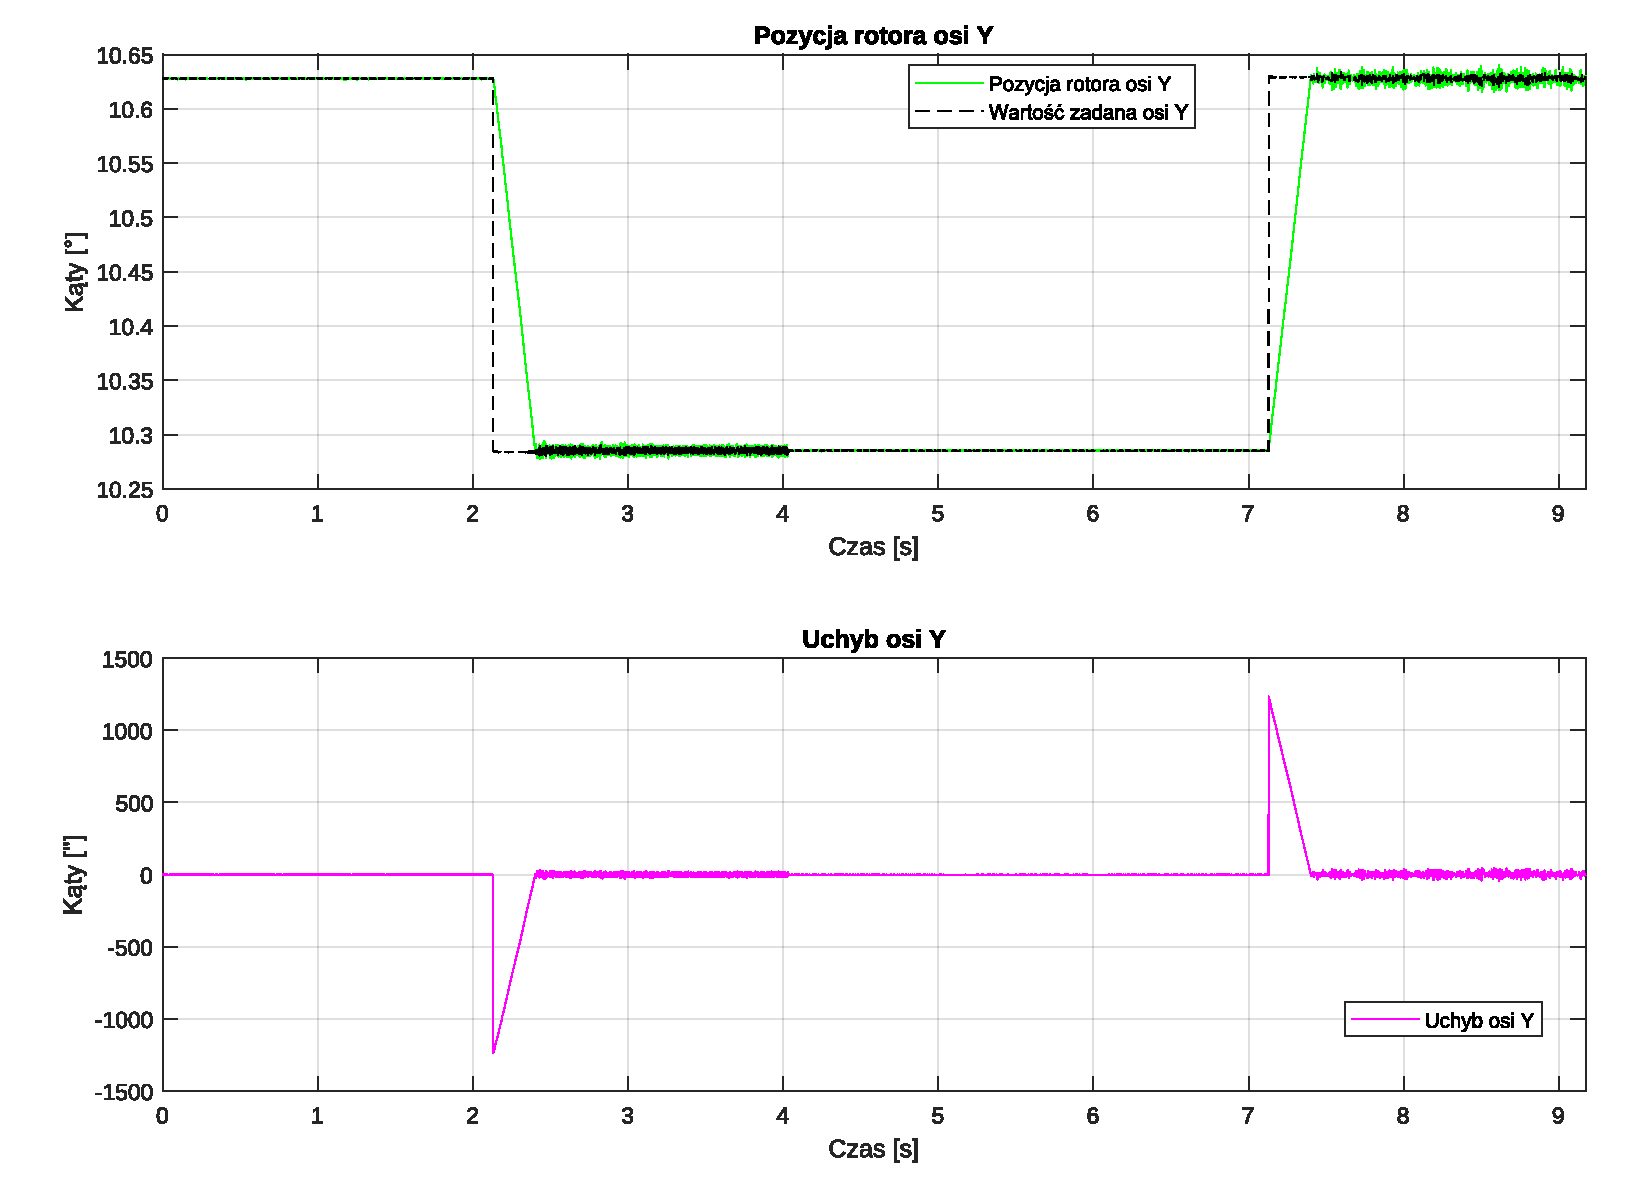
\includegraphics{testy/wykresy_inżynierka/12kY.pdf}}
    \caption{Przebiegi dla sterowania z częstotliwością 12000 Hz na osi Y.}
    \label{fig:schemat blokowy pobierania danych2}
\end{figure}

\vspace{1cm}

Zwiększając częstotliwość sygnału zegarowego podawanego na wejście CLK sterownika silnika można zauważyć, że po osiągnięciu zadanej pozycji system nie zapewniał poprawnej stabilizacji. Częstotliwość impulsów była na tyle duża, że silnik zaczynał gubić kroki, co rozsynchronizowywało pracę systemu i spowodowało zwiększenie błędu pozycjonowania. W takich warunkach odnotowano charakterystyczny dźwięk wydawany przez elementy konstrukcyjne układ napędowego w postaci ,,stukania'' i ,,pukania''. W ten sposób zaobserwowano graniczną wartość częstotliwości sygnału CLK, przy której jeszcze układ regulacji sterujący konstrukcją badanego uchwytu pracuje prawidłowo.

\section{Stany sygnału sterującego silnikiem}

\begin{figure}[H]
    \centering
    \resizebox{12cm}{!}{
    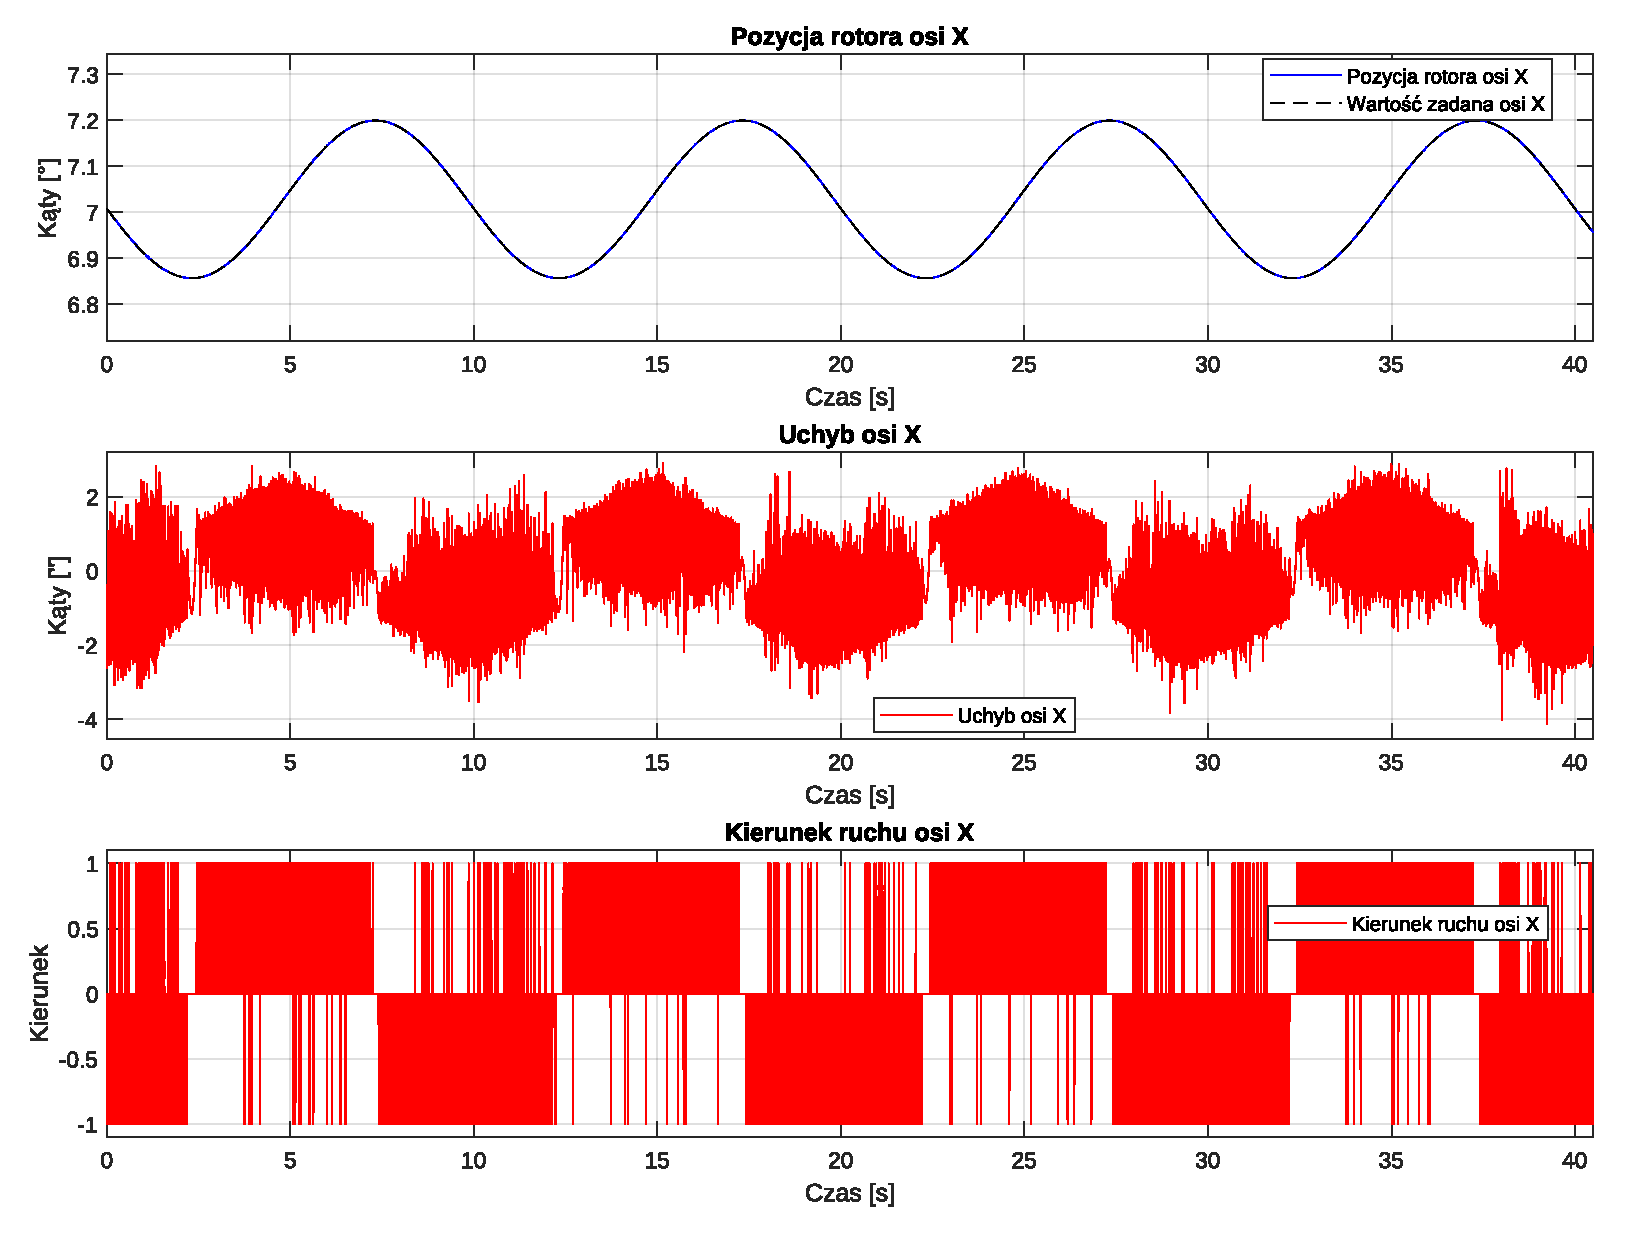
\includegraphics{testy/wykresy_inżynierka/sygnalKierunkowySin10skierunek.pdf}}
    \caption{Przebiegi dla trajektorii sinusoidalnej o okresie 10 sekund na osi X.}
    \label{fig:ster1}
\end{figure}

\begin{figure}[H]
    \centering
    \resizebox{12cm}{!}{
    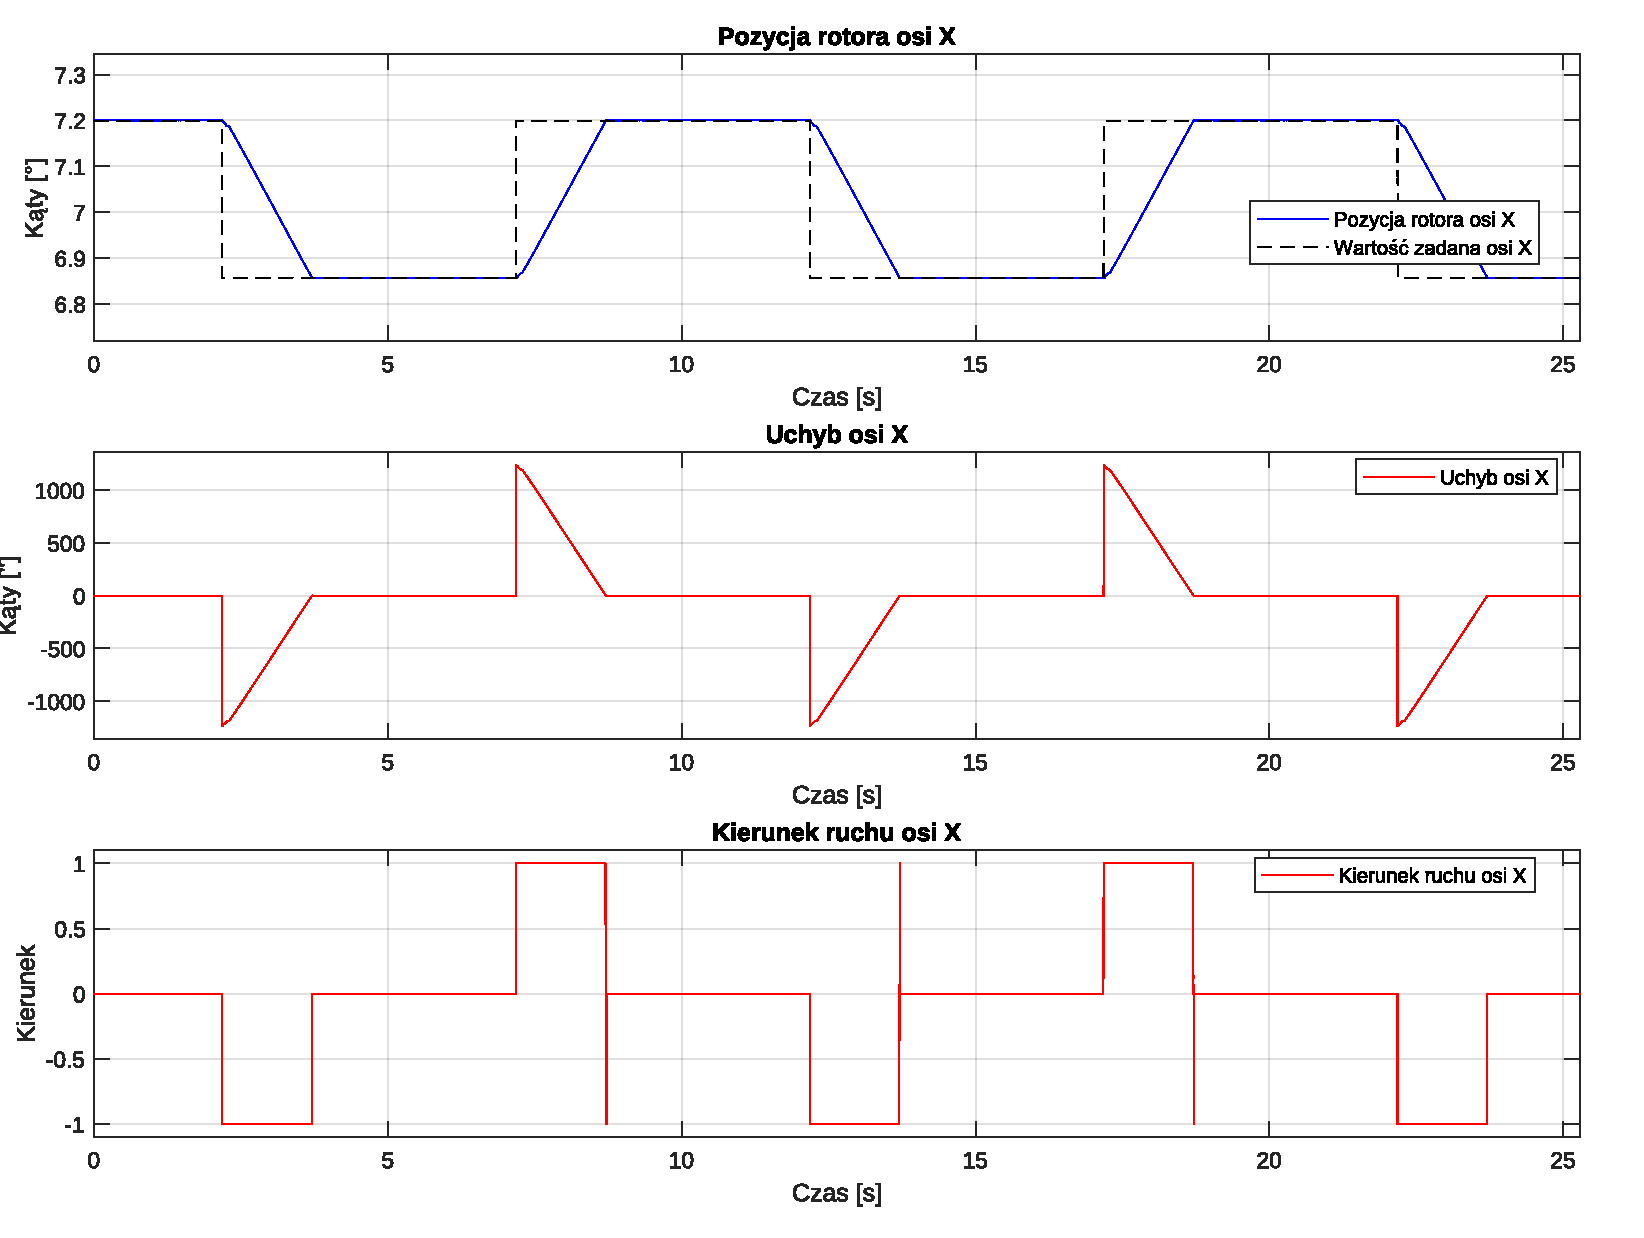
\includegraphics{testy/wykresy_inżynierka/sygnalKierunkowySquarekierunek.pdf}}
    \caption{Przebiegi dla trajektorii prostokątnej o okresie 10 sekund na osi X.}
    \label{fig:ster2}
\end{figure}
Ze względu na ograniczone zasoby mikrokontrolera test z kierunkiem ruchu został wykonany tylko na osi X. Kierunek ruchu osi X na rysunkach \ref{fig:ster1} i \ref{fig:ster2} oznaczono za pomocą następujących wartości liczbowych:
\vspace{0.5cm}
\begin{itemize}
    \item \textbf{1}: Ruch do przodu.
    \item \textbf{0}: Brak ruchu.
    \item \textbf{-1}: Ruch wsteczny.
\end{itemize}
\vspace{0.5cm}
W idealnym przypadku ruch silnika krokowego powinien odbywać się tylko w jednym kierunku w celu uzyskania stałej pozycji zadanej. Wyniki eksperymentalne pokazują, że w praktyce zachodzi potrzeba wielokrotnych zmian kierunku z uwagi na występujące oscylacje, szumy pomiarowe oraz użytą trajektorie referencyjną. Z powodu braku histerezy widoczne są szybkie zmiany kierunku na granicach wyznaczanych przez strefę nieczułości. Zjawisko to jest szczególnie widoczne przy użyciu trajektorii prostokątnej. Gdy układ osiąga pozycję zadaną, następuje korekta, a po niej system się stabilizuje i ruch ustaje.